\chapter{Euclidean geometry}
\setcounter{figure}{1}
\setcounter{subfigure}{1}
\section {Revision}
\setcounter{figure}{1}
\setcounter{subfigure}{1}

Geometry (from the Greek ``geo'' = earth and ``metria'' = measure) arose as the field of knowledge
dealing with spatial relationships. Geometry can be split into Euclidean geometry and analytical geometry. 
Analytical geometry deals with space and shape using algebra and a coordinate system. 
Euclidean geometry deals with space and shape using a system of logical deductions.\par 
\chapterstartvideo{VMchw}
\subsection*{Angles}
An angle is formed when two straight lines meet at a point, also known as a vertex. 
Angles are labelled with a caret on a letter, for example, $\hat{B}$.
Angles can also be labelled according to the line segments that make up the
angle, for example, $C\hat{B}A$ or $A\hat{B}C$. 
The $\angle $ symbol is a short method of writing angle in
geometry and is often used for phrases such as ``sum of $\angle$s in a $\triangle$''.
Angles are measured in degrees which is denoted by $^{\circ }$, a small circle
raised above the text, similar to an exponent.\par 

\Note{Angles can also be measured in radians. In high school you will use
degrees only, so make sure that your calculator is set to ``deg'' mode.}

\par 
\setcounter{subfigure}{0}
\begin{figure}[H]
\begin{center}
\begin{pspicture}(0,-1.1732812)(3.1509376,1.1732812)
\psline[linewidth=0.04](0.2465625,-0.59328127)(2.7065625,0.94671875)
\psline[linewidth=0.04](0.2465625,-0.59328127)(2.8065624,-1.0132812)
\psarc[linewidth=0.04](0.8565625,-0.46328124){0.25}{289.65384}{82.874985}
% % \usefont{T1}{ptm}{m}{n}
\rput(2.9871874,-1.0232812){$A$}
% % \usefont{T1}{ptm}{m}{n}
\rput(2.871875,0.9767187){$C$}
% % \usefont{T1}{ptm}{m}{n}
\rput(0.0459375,-0.60328126){$B$}
\end{pspicture}
% \caption{Angle labelled as $\hat{B}$, $\angle CBA$ or $\angle ABC$}
\label{fig:mg:f:ma}
\end{center}
\end{figure} 
%       
% \setcounter{subfigure}{0}
% \begin{figure}[H] % horizontal\label{m39370*uid10}
% \begin{center}
% \rule[.1in]{\figurerulewidth}{.005in} \\
% \label{m39370*uid10!!!underscore!!!media}\label{
% m39370*uid10!!!underscore!!!printimage}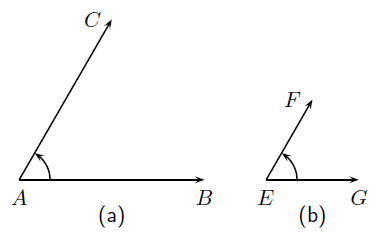
\includegraphics{
% col11306.imgs/m39370_MG10C13_003.png} % m39370;MG10C13\_003.png;;;6.0;8.5;
% \vspace{2pt}
% \vspace{\rubberspace}\par \begin{cnxcaption}
% \small \textbf{Figure 12.3: }Examples of angles. $\hat{A}=\hat{E}$, even though
% the lines making up the angles are of different lengths.
% \end{cnxcaption}
% \vspace{.1in}
% \rule[.1in]{\figurerulewidth}{.005in} \\
% \end{center}
% \end{figure}       
% \subsubsection{ Measuring angles}
% \nopagebreak
% The size of an angle does not depend on the length of the lines that are joined
% to make up the angle, but depends only on how both the lines are placed as can
% be seen in Figure~12.3. This means that the idea of length cannot be used to
% measure angles. An angle is a rotation around the vertex.\par 
% 
% \subsubsection{ Using a Protractor}
% \nopagebreak
% A protractor is a simple tool that is used to measure angles. A picture of a
% protractor is shown in Figure~12.4.\par 
% \setcounter{subfigure}{0}
% \begin{figure}[H] % horizontal\label{m39370*uid13}
% \begin{center}
% \rule[.1in]{\figurerulewidth}{.005in} \\
% \label{m39370*uid13!!!underscore!!!media}\label{
% m39370*uid13!!!underscore!!!printimage}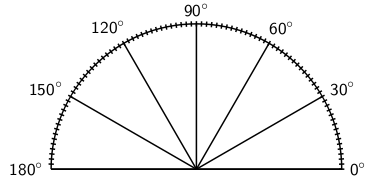
\includegraphics{
% col11306.imgs/m39370_MG10C13_004.png} % m39370;MG10C13\_004.png;;;6.0;8.5;
% \vspace{2pt}
% \vspace{\rubberspace}\par \begin{cnxcaption}
% \small \textbf{Figure 12.4: }Diagram of a protractor.
% \end{cnxcaption}
% \vspace{.1in}
% \rule[.1in]{\figurerulewidth}{.005in} \\
% \end{center}
% \end{figure}       
% 
% \textbf{Method:}
% \par 
% Using a protractor\par 
% \begin{enumerate}[noitemsep, label=\textbf{\arabic*}. ] 
% \item Place the bottom line of the protractor along one line of the angle so
% that the other line of the angle points at the degree markings.
% \item Move the protractor along the line so that the centre point on the
% protractor is at the vertex of the two lines that make up the angle.
% \item Follow the second line until it meets the marking on the protractor and
% read off the angle. Make sure you start measuring at 0$^{\circ }$.
% \end{enumerate}
% 
% \subsubsection{  Measuring Angles : Use a protractor to measure the following
% angles:}
% 
% 
% \setcounter{subfigure}{0}
% \begin{figure}[H] % horizontal\label{m39370*id314484}
% \begin{center}
% \label{m39370*id314484!!!underscore!!!media}\label{
% m39370*id314484!!!underscore!!!printimage}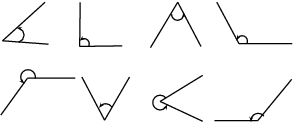
\includegraphics{
% col11306.imgs/m39370_MG10C13_005.png} % m39370;MG10C13\_005.png;;;6.0;8.5;
% \vspace{2pt}
% \vspace{.1in}
% \end{center}
% \end{figure}       
% \par 
% 
% \subsubsection{ Special Angles}
% \nopagebreak
% What is the smallest angle that can be drawn? The figure below shows two lines
% ($CA$ and $AB$) making an angle at a common vertex $A$. If line $CA$ is rotated
% around the common vertex $A$, down towards line $AB$, then the smallest angle
% that can be drawn occurs when the two lines are pointing in the same direction.
% This gives an angle of 0$^{\circ }$. This is shown in Figure~12.6\par 
% 
% \setcounter{subfigure}{0}
% \begin{figure}[H] % horizontal\label{m39370*id314593}
% \begin{center}
% \label{m39370*id314593!!!underscore!!!media}\label{
% m39370*id314593!!!underscore!!!printimage}\includegraphics[width=.8\columnwidth]
% {col11306.imgs/m39370_MG10C13_006.png} % m39370;MG10C13\_006.png;;;6.0;8.5;
% \vspace{2pt}
% \vspace{.1in}
% \end{center}
% \end{figure}       
% \par 
% If line $CA$ is now swung upwards, any other angle can be obtained. If line $CA$
% and line $AB$ point in opposite directions (the third case in Figure~12.6) then
% this forms an angle of 180$^{\circ }$.\par 
% 
% \Tip{If three points $A$, $B$ and $C$ lie on a straight line, then the angle
% between them is 180$^{\circ }$. Conversely, if the angle between three points is
% 180$^{\circ }$, then the points lie on a straight line.}
% 
% \par
% An angle of 90$^{\circ }$ is called a right angle. A right angle is half the
% size of the angle made by a straight line (180$^{\circ }$). We say $CA$ is
% perpendicular to $AB$ or $CA\perp AB$. An angle twice the size of a straight
% line is 360$^{\circ }$. An angle measuring 360$^{\circ }$ looks identical to an
% angle of 0$^{\circ }$, except for the labelling. We call this a revolution.\par 
% \setcounter{subfigure}{0}
% \begin{figure}[H] % horizontal\label{m39370*uid18}
% \begin{center}
% \rule[.1in]{\figurerulewidth}{.005in} \\
% \label{m39370*uid18!!!underscore!!!media}\label{
% m39370*uid18!!!underscore!!!printimage}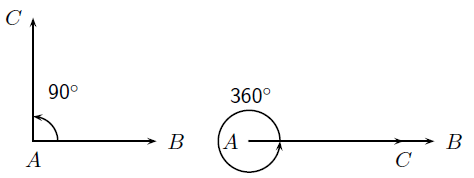
\includegraphics[width=.8\columnwidth]{
% col11306.imgs/m39370_MG10C13_007.png} % m39370;MG10C13\_007.png;;;6.0;8.5;
% \vspace{2pt}
% \vspace{\rubberspace}\par \begin{cnxcaption}
% \small \textbf{Figure 12.7: }An angle of 90$^{\circ }$ is known as a right
% angle.
% \end{cnxcaption}
% \vspace{.1in}
% \rule[.1in]{\figurerulewidth}{.005in} \\
% \end{center}
% \end{figure}       
% 
% \subsubsection{  Angles larger than 360$^{\circ }$ }
% \nopagebreak
% All angles larger than 360$^{\circ }$ also look like we have seen them before.
% If you are given an angle that is larger than 360$^{\circ }$, continue
% subtracting 360$^{\circ }$ from the angle, until you get an answer that is
% between 0$^{\circ }$and 360$^{\circ }$. Angles that measure more than
% 360$^{\circ }$ are largely for mathematical convenience. \par 
% 
% \Tip{
% \begin{itemize}[noitemsep]
% \item Acute angle: An angle $\ge {0}^{\circ }$ and $<{90}^{\circ }$.
% \item Right angle: An angle measuring ${90}^{\circ }$.
% \item Obtuse angle: An angle $>{90}^{\circ }$ and $<{180}^{\circ }$.
% \item Straight angle: An angle measuring 180$^{\circ }$.
% \item Reflex angle: An angle $>{180}^{\circ }$ and $<{360}^{\circ }$.
% \item Revolution: An angle measuring ${360}^{\circ }$.
% \end{itemize}
% These are simply labels for angles in particular ranges, shown in Figure~12.8.}
% \par
% \setcounter{subfigure}{0}
% \begin{figure}[H] % horizontal\label{m39370*uid25}
% \begin{center}
% \rule[.1in]{\figurerulewidth}{.005in} \\
% \label{m39370*uid25!!!underscore!!!media}\label{
% m39370*uid25!!!underscore!!!printimage}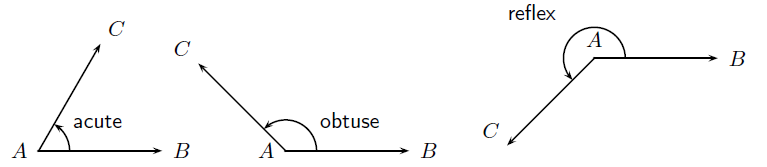
\includegraphics[width=.8\columnwidth]{
% col11306.imgs/m39370_MG10C13_008.png} % m39370;MG10C13\_008.png;;;6.0;8.5;
% \vspace{2pt}
% \vspace{\rubberspace}\par \begin{cnxcaption}
% \small \textbf{Figure 12.8: }Three types of angles defined according to their
% ranges.
% \end{cnxcaption}
% \vspace{.1in}
% \rule[.1in]{\figurerulewidth}{.005in} \\
% \end{center}
% \end{figure}       
% Once angles can be measured, they can then be compared. For example, all right
% angles are 90$^{\circ }$, therefore all right angles are equal and an obtuse
% angle will always be larger than an acute angle.\par The following video
% summarizes what you have learnt so far about angles.
% \setcounter{subfigure}{0}
% \begin{figure}[H] % horizontal\label{m39370*angles-1}
% \textnormal{Khan Academy video on angles - 1}\vspace{.1in} \nopagebreak
% \label{m39370*yt-media1}\label{m39370*yt-video1}
% \raisebox{-5 pt}{ 
\includegraphics[width=0.5cm]{col11306.imgs/summary_www.png}}
% { (Video:  MG10088 )}
% \vspace{2pt}
% \vspace{.1in}
% \end{figure}       
% Note that for high school trigonometry you will be using degrees, not radians as
% stated in the video. \par 

\subsection*{Properties and notation}

In the diagram below two straight lines intersect at a point, forming the four
angles $\hat{a}$, $\hat{B}$, $\hat{c}$ and $\hat{d}$.\par 
% Need new diagram here 
\setcounter{subfigure}{0}
 	\begin{figure}[H] 
    \begin{center}
\scalebox{1.2} % Change this value to rescale the drawing.
{
\begin{pspicture}(0,-1.124111)(4.2,1.124111)
\psline[linewidth=0.028222222cm,arrowsize=0.05291667cm 2.0,arrowlength=1.4,arrowinset=0.4]{<->}(0.08588889,-1.11)(4.145889,1.11)
\psline[linewidth=0.028222222cm,arrowsize=0.05291667cm 2.0,arrowlength=1.4,arrowinset=0.4]{<->}(0.0,0.9358889)(4.185889,-1.05)
\psarc[linewidth=0.028222222](2.1029444,-0.011166667){0.58294445}{330.0}{30.0}
\psarc[linewidth=0.028222222](1.9629444,-0.057055555){0.53705555}{150.0}{210.0}
\psarc[linewidth=0.028222222](2.0679445,-0.022055555){0.42205554}{30.0}{157.48302}
\psarc[linewidth=0.028222222](2.0579445,-0.012055555){0.47205555}{210.0}{330.0}
\psarc[linewidth=0.028222222](2.0629444,-0.037055556){0.49705556}{30.0}{155.69582}
\psarc[linewidth=0.028222222](2.0529444,-0.0070555555){0.54705554}{210.0}{330.0}
% % \usefont{T1}{ptm}{m}{n}
\rput(2.4014063,-0.004111111){\small{$a$}}
% % \usefont{T1}{ptm}{m}{n}
\rput(2.0214062,0.21588889){\small{$b$}}
% % \usefont{T1}{ptm}{m}{n}
\rput(1.7014062,-0.04411111){\small{$c$}}
% % \usefont{T1}{ptm}{m}{n}
\rput(2.1014063,-0.2841111){\small{$d$}}
\end{pspicture} 
}

    \end{center}
% \caption{Two intersecting straight lines with vertical angles $\hat{A},\hat{C}$ and $\hat{B},\hat{D}$.}
\label{fig:mg:f:specialangles2}
 \end{figure}        
The following table summarises the different types of angles, with
examples from the figure above.

% \textbf{m39370*id315548}\par
\begin{table}[H]
\begin{center}
\begin{tabular}{|p{3.5cm}|p{4cm}|p{4cm}|} \hline
\textbf{Term} & \textbf{Property} & \textbf{Examples}\\ \hline
Acute angle & $0^{\circ} < \mbox{angle} < 90^{\circ}$ & $\hat{a}$; $\hat{c}$ \\ \hline
Right angle & Angle $= 90^{\circ}$ &  \\ \hline
Obtuse angle & $90^{\circ} < \mbox{angle} < 180^{\circ}$ & $\hat{b}$; $\hat{d}$ \\ \hline
Straight angle & Angle $= 180^{\circ}$ & $\hat{a} + \hat{b}$;  $\hat{b} + \hat{c}$  \\
& &  \\ \hline
Reflex angle & $180^{\circ} < \mbox{angle} < 360^{\circ}$ & $\hat{a} + \hat{b} + \hat{c}$ \\ \hline
Adjacent angles & Angles that share a vertex and a common side. & $\hat{a}$ and $\hat{d}$;  $\hat{c}$ and $\hat{d}$ \\ 
& &  \\ \hline
Vertically opposite angles & Angles opposite each other when two lines intersect. They share a vertex and are equal. & $\hat{a}=\hat{c}$;  $\hat{b}=\hat{d}$\\
 &  & \\ \hline
Supplementary angles & Two angles that add up to $180^{\circ}$. & $\hat{a}+\hat{b}=180^{\circ}$; $\hat{b}+\hat{c}=180^{\circ}$ \\ 
& &  \\ \hline
Complementary angles & Two angles that add up to $90^{\circ}$. & \\ \hline
Revolution & The sum of all angles around a point. &  $\hat{a}+\hat{b}+\hat{c}+\hat{d}=360^{\circ}$ \\ \hline

\end{tabular}
\end{center}
\end{table}
\par

\Note{Adjacent angles on a straight line are supplementary.}
% The following video summarises what you have learnt so far
% \setcounter{subfigure}{0}
% \begin{figure}[H] % horizontal\label{m39370*angles-2}
% \textnormal{Khan Academy video on angles - 2}\vspace{.1in} \nopagebreak
% \label{m39370*yt-media2}\label{m39370*yt-video2}
% \raisebox{-5 pt}{ 
\includegraphics[width=0.5cm]{col11306.imgs/summary_www.png}}
% { (Video:  MG10089 )}
% \vspace{2pt}
% \vspace{.1in}
% \end{figure}      

\subsection*{Parallel lines and transversal lines}
Two lines intersect if they cross each other at a point. For example, at a
traffic intersection two or more streets intersect; the middle of the
intersection is the common point between the streets.

Parallel lines are always the same distance apart and they are denoted
by arrow symbols as shown below.

\setcounter{subfigure}{0}
\begin{figure}[H]
 \begin{center}
\scalebox{1}{
  \begin{pspicture}(0,0)(5,5)
%Lines MN and OP
\psline[linewidth=0.04cm](0,0)(5,3)
\psline[linewidth=0.01cm,arrowsize=0.2cm 2.0,arrowlength=1.4,arrowinset=0.5]{->}(2.3,1.4)(2.7,1.6)
\psline[linewidth=0.04cm](0.5,-.5)(5.5,2.5)
\psline[linewidth=0.01cm,arrowsize=0.2cm 2.0,arrowlength=1.4,arrowinset=0.5]{->}(2.5,0.7)(2.8,.9)
%Lines AB and CD
\psline[linewidth=0.04cm](2.5,-.5)(0.5,2.5)
\psline[linewidth=0.01cm,arrowsize=0.2cm 2.0,arrowlength=1.4,arrowinset=0.5]{->>}(2.5,-0.5)(2.2,0)
\psline[linewidth=0.04cm](5,0)(3,3)
\psline[linewidth=0.01cm,arrowsize=0.2cm 2.0,arrowlength=1.4,arrowinset=0.5]{->>}(4.6,0.6)(4.3,1.1)
%And the labels
\rput[t](0.5,2.8){$M$}
\rput[b](2.5,-.8){$N$}
\rput[b](5,-.3){$P$}
\rput[t](3,3.3){$O$}
\rput[l](-.3,0){$A$}
\rput[r](5.3,3){$B$}
\rput[l](0.2,-.5){$C$}
\rput[r](5.8,2.5){$D$}
  \end{pspicture}
}  
 \end{center}
\end{figure} 

In writing we use two vertical lines to indicate that two lines are
parallel:
\begin{equation*}
  AB \parallel CD \mbox{ and } MN \parallel OP
\end{equation*}

\Note{A section of the Australian National Railways Trans-Australian line is perhaps
one of the longest pairs of man-made parallel lines.
The Australian National Railways Trans-Australian line over the Nullarbor Plain,
is 478~km (297 miles) dead straight, from Mile 496, between Nurina and Loongana,
Western Australia, to Mile 793, between Ooldea and Watson, South
Australia. (Source: Guinness World Records)} % end \textsl

A transversal line intersects two or more parallel lines. In the diagram below, $AB \parallel CD$ and $EF$ is a
transversal line. The properties of the angles formed by these intersecting lines are summarised in the following table:\par 
\setcounter{subfigure}{0}
\begin{figure}[htb]
\begin{center}
\begin{pspicture}(0,-1.5)(6,3.5)
%\psgrid[gridcolor=lightgray]
\psline{-}(0,0)(6,0)
\psline[linewidth=0.01cm,arrowsize=0.2cm 2.0,arrowlength=1.4,arrowinset=0.5]{->}(0,0)(1.5,0)
\uput[l](0,0){$A$}
\uput[r](6,0){$B$}
\psline{-}(0,2)(6,2)
\psline[linewidth=0.01cm,arrowsize=0.2cm 2.0,arrowlength=1.4,arrowinset=0.5]{->}(0,2)(1.5,2)
\uput[l](0,2){$C$}
\uput[r](6,2){$D$}
\psline{-}(1,-1)(5,3)
\uput[dl](1,-1){$E$}
\uput[ur](5,3){$F$}

\psarc(4,2){0.5}{0}{45} \uput{0.6}[22.5](4,2){$g$}
\psarc(4,2){0.3}{45}{180} \psarc(4,2){0.4}{45}{180} \uput{0.5}[112.5](4,2){$h$}
\psarc(4,2){0.5}{180}{225} \uput{0.6}[202.5](4,2){$a$}
\psarc(4,2){0.3}{225}{360} \psarc(4,2){0.4}{225}{360} \uput{0.5}[292.5](4,2){$b$}
\psarc(2,0){0.5}{0}{45} \uput{0.6}[22.5](2,0){$c$}
\psarc(2,0){0.3}{45}{180} \psarc(2,0){0.4}{45}{180} \uput{0.5}[112.5](2,0){$d$}
\psarc(2,0){0.5}{180}{225} \uput{0.6}[202.5](2,0){$e$}
\psarc(2,0){0.3}{225}{360} \psarc(2,0){0.4}{225}{360} \uput{0.5}[292.5](2,0){$f$}
\end{pspicture}
% \caption{Parallel lines intersected by a transversal}
\label{fig:mg:f:partrans}
\end{center}
\end{figure}      
% \textbf{m39370*uid30}\par
\begin{table}[H]
\begin{center}
%\caption{Properties of angles formed when parallel lines are intersected by a transversal. The example in Figure~\ref{fig:mg:f:partrans} is used as a reference.}
\label{tab:mg:f:partrans}
\begin{tabular}{|p{2.25cm}|p{4cm}|p{3cm}|p{2.5cm}|}\hline
\textbf{Name of angle} & \textbf{Definition} & \textbf{Examples} & \textbf{Notes}\\\hline
Interior angles & Angles that lie in between the parallel lines. & $\hat{a}$, $\hat{b}$, $\hat{c}$ and $\hat{d}$ are interior angles. & Interior means inside. \\ \hline
Exterior angles & Angles that lie outside the parallel lines. & $\hat{e}$, $\hat{f}$, $\hat{g}$ and $\hat{h}$ are exterior angles. & Exterior means outside. \\ \hline
Corresponding angles &
Angles on the same side of the lines and the same side of the
transversal. If the lines are parallel, the corresponding angles will
be equal. &
$\hat{a}$ and $\hat{e}$,  $\hat{b}$ and $ \hat{f}$,  $\hat{c} $ and $
\hat{g}$, $\hat{d}$ and $ \hat{h}$ are pairs of corresponding
angles. $\hat{a}=\hat{e}$,  $\hat{b}= \hat{f}$,  $\hat{c} = \hat{g}$,
$\hat{d}= \hat{h}$. &
\raisebox{-.8\height}{
%\scalebox{1} % Change this value to rescale the drawing.
% \begin{center}
%{
\begin{pspicture}(0,-0.9884375)(1.48,0.7884375)
\psline[linewidth=0.04cm](0.2,0.7684375)(1.46,0.7684375)
\psline[linewidth=0.04cm](0.22,0.1284375)(1.44,0.1284375)
\psline[linewidth=0.01cm,arrowsize=0.2cm 2.0,arrowlength=1.4,arrowinset=0.5]{->>}(0.38,0.1284375)(1.16,0.1284375)
\psline[linewidth=0.01cm,arrowsize=0.2cm 2.0,arrowlength=1.4,arrowinset=0.5]{->>}(0.22,0.7684375)(1.0,0.7684375)
% % \usefont{T1}{ptm}{m}{n}
\rput(0.7128125,-0.7615625){F shape}
\psline[linewidth=0.04cm](0.2,0.7684375)(0.2,-0.5315625)
\psarc[linewidth=0.04](0.2,0.7484375){0.2}{270.0}{0.0}
\psarc[linewidth=0.04](0.22,0.1084375){0.2}{270.0}{0.0}
\end{pspicture} 
% \end{center}
}
%}
\\\hline
Co-interior angles &
Angles that lie in between the parallel lines and on the same side of
the transversal. If the lines are parallel, the angles are
supplementary. &
$\hat{a}$ and $\hat{d}$, $\hat{b}$ and $\hat{c}$ are pairs of
co-interior angles. $\hat{a} + \hat{d} = 180^{\circ}$, $\hat{b} +
\hat{c} = 180^{\circ}$. &
\raisebox{-.8\height}{
%\scalebox{1} % Change this value to rescale the drawing.
%{
\begin{pspicture}(0,-0.8384375)(1.64,0.6513173)
\psline[linewidth=0.04cm](0.24,0.6184375)(1.5,0.6184375)
\psline[linewidth=0.04cm](0.26,-0.3415625)(1.62,-0.3415625)
\psline[linewidth=0.01cm,arrowsize=0.2cm 2.0,arrowlength=1.4,arrowinset=0.5]{->>}(0.42,-0.3415625)(1.2,-0.3415625)
\psline[linewidth=0.01cm,arrowsize=0.2cm 2.0,arrowlength=1.4,arrowinset=0.5]{->>}(0.26,0.6184375)(1.04,0.6184375)
\psarc[linewidth=0.04](0.24,-0.3815625){0.24}{7.125016}{90.0}
% % \usefont{T1}{ptm}{m}{n}
\rput(0.83671874,-0.8){C shape}
\psline[linewidth=0.04cm](0.24,0.6184375)(0.24,-0.3615625)
\psarc[linewidth=0.04](0.24,0.5984375){0.2}{270.0}{9.462322}
\end{pspicture} }
%}
\\\hline
Alternate interior angles &
Equal interior angles that lie inside the line and on opposite sides
of the transversal. If the lines are parallel, the interior angles
will be equal. &
$\hat{a}$ and $\hat{c}$, $\hat{b}$ and $\hat{d}$ are pairs of
alternate interior angles. $\hat{a} = \hat{c}$, $\hat{b} = \hat{d}$. &
% \begin{center}
\raisebox{-.8\height}{
%\scalebox{1} % Change this value to rescale the drawing.
%{
\begin{pspicture}(0,-0.8184375)(1.4,0.6584375)
\psline[linewidth=0.04cm](0.0,0.6384375)(1.26,0.6384375)
\psline[linewidth=0.04cm](1.26,0.6384375)(0.02,-0.3215625)
\psline[linewidth=0.04cm](0.02,-0.3215625)(1.38,-0.3215625)
\psline[linewidth=0.01cm,arrowsize=0.2cm 2.0,arrowlength=1.4,arrowinset=0.5]{->>}(0.18,-0.3215625)(0.96,-0.3215625)
\psline[linewidth=0.01cm,arrowsize=0.2cm 2.0,arrowlength=1.4,arrowinset=0.5]{->>}(0.02,0.6384375)(0.8,0.6384375)
\psarc[linewidth=0.04](1.06,0.5784375){0.2}{168.69006}{243.43495}
\psarc[linewidth=0.04](0.2465625,-0.215){0.2265625}{329.03625}{45.0}
% % \usefont{T1}{ptm}{m}{n}
\rput(0.591875,-0.8){Z shape}
\end{pspicture} }
%
% \end{center}
\\\hline
\end{tabular}
\end{center}
\end{table}

If two lines are intersected by a transversal such that
\begin{itemize}[noitemsep]
\item corresponding angles are equal; or
\item alternate interior angles are equal; or
\item co-interior angles are supplementary
\end{itemize}
then the two lines are parallel.

% \begin{figure}[H] % horizontal\label{m38380*angles-3}    
% \textnormal{Khan Academy video on angles - 3}
% \label{m38380*yt-media3}\label{m38380*yt-video3}
%     \raisebox{-0.2em}{
\includegraphics[height=1em]{../icons/www.pdf}}{ (Video:  P10116)}
% \end{figure} 


%  %MANUAL PGBREAK TO FORCE WEX BELOW TO SPLIT (still doesnt split properly. Damn mdframed!!!)
\begin{wex}{Finding angles}
{Find all the unknown angles. Is $EF \parallel CG$? Explain your answer.
 \begin{center}
   \scalebox{0.9} % Change this value to rescale the drawing.
{
\begin{pspicture}(0,-2.57375)(12.675937,2.57375)
\psline[linewidth=0.01cm,arrowsize=0.2cm 2.0,arrowlength=1.4,arrowinset=0.5]{->}(3.68,0.07124995)(4.32,0.43124995)
\psline[linewidth=0.01cm,arrowsize=0.2cm 2.0,arrowlength=1.4,arrowinset=0.5]{->}(8.18,-0.18875004)(8.8,0.17124996)
\rput{-143.0545}(8.17638,3.9190145){\psarc[linewidth=0.04](4.742796,0.5937799){0.49404234}{343.58032}{85.22324}}
\psline[linewidth=0.04cm](0.0,-2.14875)(6.62,1.83125)
\psline[linewidth=0.04cm](4.96,-2.12875)(12.14,2.23375)
\psline[linewidth=0.04cm](2.96,-2.10875)(9.0,-2.10875)
\psline[linewidth=0.04cm](4.96,-2.10875)(5.0,0.89124984)
\psline[linewidth=0.04cm](2.44,-0.64875007)(12.48,1.53375)
\psline[linewidth=0.04cm](4.8,-2.0887501)(4.8,-1.96875)
\psline[linewidth=0.04cm](4.78,-1.94875)(4.98,-1.94875)
% \usefont{T1}{ptm}{m}{n}
\rput(4.7,0.44624996){\footnotesize $60^{\circ}$}
\psbezier[linewidth=0.04](1.94,-1.0062499)(2.46,-1.52625)(3.24,-1.02625)(3.18,-0.52624995)
% \usefont{T1}{ptm}{m}{n}
\rput{0.86235595}(-0.013302135,-0.039991397){\rput(2.623804,-0.9042548){\footnotesize $160^{\circ}$}}
\psarc[linewidth=0.04](5.09,-1.7787501){0.39}{351.02737}{104.74356}
\rput{-33.527527}(1.9972864,2.8241615){\psarc[linewidth=0.04](5.6863933,-1.9031615){0.33947578}{0.0}{99.46232}}
\rput{-210.4531}(17.459091,-3.5844944){\psarc[linewidth=0.04](9.217381,0.58386225){0.3534083}{0.0}{78.96434}}
\rput{-28.674759}(0.6394295,5.5710244){\psarc[linewidth=0.04](11.218004,1.5346314){0.32564545}{343.67474}{75.4531}}
\psbezier[linewidth=0.04](9.8,0.7850357)(10.352,0.33375004)(10.9,0.71375006)(10.96,1.21375)
% \usefont{T1}{ptm}{m}{n}
\rput(5.1759377,-1.67875){$x$}
% \usefont{T1}{ptm}{m}{n}
\rput(5.6659374,-1.8987501){$s$}
% \usefont{T1}{ptm}{m}{n}
\rput(9.165937,0.64){$y$}
% \usefont{T1}{ptm}{m}{n}
\rput(10.395937,0.88124996){$r$}
% \usefont{T1}{ptm}{m}{n}
\rput(11.285938,1.5012499){$p$}
% \usefont{T1}{ptm}{m}{n}
\rput(4.862969,-2.41875){$C$}
% \usefont{T1}{ptm}{m}{n}
\rput(9.175625,-2.27875){$G$}
% \usefont{T1}{ptm}{m}{n}
\rput(12.290313,2.3812501){$D$}
% \usefont{T1}{ptm}{m}{n}
\rput(12.525156,1.34125){$F$}
% \usefont{T1}{ptm}{m}{n}
\rput(0.186875,-2.3387501){$A$}
% \usefont{T1}{ptm}{m}{n}
\rput(2.3165624,-0.35875005){$E$}
% \usefont{T1}{ptm}{m}{n}
\rput(4.8403125,1.18125){$B$}
\end{pspicture} 
 
}
 \end{center}
} 
{\westep{Use the properties of parallel lines to find all equal angles on the diagram}

\westep{Determine the unknown angles}
\begin{equation*}
  \begin{array}{r@{\;}l@{\quad}l}
    AB  &\parallel CD & \mbox{(given)} \\
    \therefore \hat{x} &=60^{\circ}   & \mbox{(alt.\ int.\ $\angle$'s)}  \vspace{10pt} \\
    \hat{y} + 160^\circ &= 180^{\circ} & \mbox{(co-int.\ $\angle$'s)} \\
    \therefore \hat{y} &= 20^{\circ}  & \vspace{8pt}\\
    \hat{p} &= \hat{y}    & \mbox{(vert.\ opp.\ $\angle$'s)} \\
    \therefore \hat{p} &= 20^{\circ}  &  \vspace{10pt}\\
    \hat{r} + \hat{p} &= 180^{\circ} &\mbox{(sum of $\angle$'s str.\ line)} \\
    \therefore \hat{r} &= 160^{\circ} &  \vspace{10pt}\\
    \hat{s} + \hat{x} &= 90^{\circ}  & \mbox{(given)} \\ 
    \hat{s} + 60^\circ &= 90^{\circ} & \\
    \therefore \hat{s} &= 30^{\circ} &  
  \end{array}
\end{equation*} 
\westep{Determine whether $EF \parallel CG$}

If $EF \parallel CG$ then $\hat{p}$ will be equal to corresponding
angle $\hat{s}$, but $\hat{p} = 20^{\circ}$ and $\hat{s} = 30^{\circ}$.
Therefore $EF$ is not parallel to $CG$.
}
\end{wex}


\begin{exercises}{}{
\begin{enumerate}[label=\textbf{\arabic*}.]
\item Use adjacent, corresponding, co-interior and alternate angles to fill in all the angles labelled with letters in the diagram:\\
\begin{pspicture}(0,-1.7981373)(6.5116725,1.7981373)
\psline[linewidth=0.04cm](0.34542254,0.6181373)(5.2654223,0.6181373)
\psline[linewidth=0.04cm](0.34542254,-0.7418627)(5.2654223,-0.7418627)
\psline[linewidth=0.04cm](0.0,-1.7781373)(5.5254226,1.7781373)
% % \usefont{T1}{ptm}{m}{n}
\rput(4.4,0.8){\footnotesize$42^\circ$}
% % \usefont{T1}{ptm}{m}{n}
\rput(3.664485,0.8881373){$a$}
% \usefont{T1}{ptm}{m}{n}
\rput(3.0458913,0.3881373){$b$}
% \usefont{T1}{ptm}{m}{n}
\rput(3.8072975,0.4081373){$c$}
% \usefont{T1}{ptm}{m}{n}
\rput(1.5262038,-0.5518627){$d$}
% \usefont{T1}{ptm}{m}{n}
\rput(2.2315164,-0.5518627){$e$}
% \usefont{T1}{ptm}{m}{n}
\rput(1.6212038,-1.0518627){$f$}
% \usefont{T1}{ptm}{m}{n}
\rput(1.05,-0.95){$g$}
\rput{-66.70425}(1.9155159,4.522671){\psarc[linewidth=0.032]{-}(4.3934965,0.8061751){0.24084859}{20.012312}{156.69316}}
\psline[linewidth=0.04](3.9254224,-0.6018627)(4.2254224,-0.7418627)(3.9454224,-0.8818627)
\psline[linewidth=0.04](3.6854224,-0.6018627)(3.9854226,-0.7418627)(3.7054226,-0.8818627)
\psline[linewidth=0.04](2.2454226,0.7581373)(2.5454226,0.6181373)(2.2654226,0.47813728)
\psline[linewidth=0.04](2.0054226,0.7581373)(2.3054225,0.6181373)(2.0254226,0.47813728)
\end{pspicture}
\\
\item Find all the unknown angles in the figure: \\
\\
\scalebox{1.2}{
\begin{pspicture}(0,-1.6967187)(5.5376563,1.7167188)
\psline[linewidth=0.04cm](3.1065626,1.4032813)(5.0465627,-1.4567187)
\psline[linewidth=0.04cm](0.4665625,1.1832813)(2.4065626,-1.6767187)
\psline[linewidth=0.01cm,arrowsize=0.2cm 2.0,arrowlength=1.4,arrowinset=0.5]{->>}(0.49,1.1417187)(1.3465625,-0.11671878)
\psline[linewidth=0.01cm,arrowsize=0.2cm 2.0,arrowlength=1.4,arrowinset=0.5]{->>}(3.3065624,1.1032813)(4.29,-0.29828128)
\psline[linewidth=0.04cm](1.5065625,-0.3367187)(4.4465623,-0.5567187)
\psline[linewidth=0.04cm](0.8665625,0.6232813)(3.8065624,0.40328127)
\psline[linewidth=0.01cm,arrowsize=0.2cm 2.0,arrowlength=1.4,arrowinset=0.5]{->}(1.5265626,-0.33671877)(3.1265626,-0.47671878)
\psline[linewidth=0.01cm,arrowsize=0.2cm 2.0,arrowlength=1.4,arrowinset=0.5]{->}(1.0065625,0.62328136)(2.77,0.48171872)
\psline[linewidth=0.04cm](3.7665625,0.40328127)(1.5065625,-0.3367187)
\psline[linewidth=0.04cm](4.4065623,-0.5567187)(2.1465626,-1.2967187)
\psline[linewidth=0.01cm,arrowsize=0.2cm 2.0,arrowlength=1.4,arrowinset=0.5]{->}(3.2065625,0.22328123)(2.3665626,-0.09671878)
\psline[linewidth=0.01cm,arrowsize=0.2cm 2.0,arrowlength=1.4,arrowinset=0.5]{->}(3.4065626,0.30328122)(2.5665624,-0.01671878)
\psline[linewidth=0.01cm,arrowsize=0.2cm 2.0,arrowlength=1.4,arrowinset=0.5]{->}(3.6265626,0.38328123)(2.7865624,0.06328122)
\psline[linewidth=0.01cm,arrowsize=0.2cm 2.0,arrowlength=1.4,arrowinset=0.5]{->}(3.7465625,-0.7767188)(2.89,-1.0782813)
\psline[linewidth=0.01cm,arrowsize=0.2cm 2.0,arrowlength=1.4,arrowinset=0.5]{->}(3.9465625,-0.69671875)(3.1065626,-1.0167189)
\psline[linewidth=0.01cm,arrowsize=0.2cm 2.0,arrowlength=1.4,arrowinset=0.5]{->}(4.1665626,-0.61671877)(3.3265624,-0.93671876)
\usefont{T1}{ptm}{m}{n}
\rput(0.28453124,1.1932813){$A$}
\usefont{T1}{ptm}{m}{n}
\rput(0.60765624,0.5132813){$B$}
\usefont{T1}{ptm}{m}{n}
\rput(1.3045312,-0.54627085){$C$}
\usefont{T1}{ptm}{m}{n}
\rput(1.9399999,-1.3867188){$D$}
\usefont{T1}{ptm}{m}{n}
\rput(3.2096875,1.5132812){$E$}
\usefont{T1}{ptm}{m}{n}
\rput(3.9235938,0.49328125){$F$}
\usefont{T1}{ptm}{m}{n}
\rput(4.5775,-0.46671876){$G$}
\usefont{T1}{ptm}{m}{n}
\rput(5.1331253,-1.3267187){$H$}
\usefont{T1}{ptm}{m}{n}
\rput(1.25,0.41){\tiny $70^\circ$}
\usefont{T1}{ptm}{m}{n}
\rput(2.3,-1.0917187){\tiny $80^\circ$}
\usefont{T1}{ptm}{m}{n}
\rput(0.87921876,0.7532813){\tiny $1$}
\usefont{T1}{ptm}{m}{n}
\rput(3.4192188,0.61328125){\tiny $1$}
\usefont{T1}{ptm}{m}{n}
\rput(3.144219,0.33328128){\tiny $2$}
\usefont{T1}{ptm}{m}{n}
\rput(3.6359375,0.21328127){\tiny $3$}
\usefont{T1}{ptm}{m}{n}
\rput(4.119219,-0.44671872){\tiny $1$}
\usefont{T1}{ptm}{m}{n}
\rput(3.7442188,-0.6667187){\tiny $2$}
\usefont{T1}{ptm}{m}{n}
\rput(4.2959375,-0.7467187){\tiny $3$}
\usefont{T1}{ptm}{m}{n}
\rput(1.5392189,-0.12671873){\tiny $1$}
\usefont{T1}{ptm}{m}{n}
\rput(2.1442187,-0.28671873){\tiny $2$}
\usefont{T1}{ptm}{m}{n}
\rput(1.7959374,-0.5667187){\tiny $3$}
\usefont{T1}{ptm}{m}{n}
\rput(2.3192186,-1.3667188){\tiny $1$}
\rput{-165.35927}(1.9916399,1.1648247){\psarc[linewidth=0.04](1.0706391,0.4544851){0.34608197}{92.73279}{185.53572}}
\rput{-45.10457}(1.5105618,1.2407944){\psarc[linewidth=0.04](2.2491949,-1.1983162){0.29357287}{50.13503}{194.957}}
\end{pspicture}
}  \\ 
\item Find the value of $x$ in the figure: \\

\scalebox{1.2} % Change this value to rescale the drawing.
{
\begin{pspicture}(0,-2.203125)(4.2173834,2.203125)
\psline[linewidth=0.04cm](0.84234375,1.8096874)(0.84234375,-1.7303125)
\psline[linewidth=0.04cm](1.8423437,1.8096874)(1.8423437,-1.7303125)
\psline[linewidth=0.04cm](0.38,0.9631251)(3.36,-0.7768749)
\psline[linewidth=0.04cm](3.94,0.6631251)(0.12,-0.4368749)
\usefont{T1}{ptm}{m}{n}
\rput(0.81859374,1.9996876){$A$}
\usefont{T1}{ptm}{m}{n}
\rput(0.77796876,-2.0003126){$B$}
\usefont{T1}{ptm}{m}{n}
\rput(1.7839063,-2.0003126){$C$}
\usefont{T1}{ptm}{m}{n}
\rput(1.7903125,1.9996876){$D$}
\usefont{T1}{ptm}{m}{n}
\rput(0.29453126,0.73968744){$X$}
\usefont{T1}{ptm}{m}{n}
\rput(1.6604688,-0.2610938){$Y$}
\usefont{T1}{ptm}{m}{n}
\rput(0.63609374,-0.5403126){$Z$}
\psline[linewidth=0.04cm](1.8423437,1.5096875)(1.9423437,1.6896875)
\psline[linewidth=0.04cm](1.8423437,1.5096875)(1.7423438,1.6696874)
\usefont{T1}{ptm}{m}{n}
\rput(1.1,-0.0){\scriptsize $60^{\circ}$}
\usefont{T1}{ptm}{m}{n}
\rput(0.9571874,0.45468745){\scriptsize $x$}
\usefont{T1}{ptm}{m}{n}
\rput{-0.80275255}(0.0,0.046365827){\rput(2.9,-0.006999445){\scriptsize $x-20^\circ$}}
\rput{-122.44731}(3.35288,1.925009){\psarc[linewidth=0.04](2.205064,0.041774992){0.20109077}{59.366795}{168.11142}}
\psline[linewidth=0.04cm](0.84234375,1.5296875)(0.9423437,1.7096875)
\psline[linewidth=0.04cm](0.84234375,1.5296875)(0.7423437,1.6896874)
\end{pspicture} 

} \\
\item Determine whether the pairs of lines in the following figures are parallel:
\begin{enumerate}[itemsep=10pt, label=\textbf{(\alph*)} ] 
\item \raisebox{-4.5cm}{
    \scalebox{1}{ % Change this value to rescale the drawing.
      \begin{pspicture}(0,-2.451875)(6.3617187,2.451875)
        \psline[linewidth=0.04cm](0.0,1.6081251)(6.1,-1.751875)
        \psline[linewidth=0.04cm](1.42,2.171875)(1.74,-1.808125)
        \psline[linewidth=0.04cm](4.72,2.188125)(5.08,-2.211875)
        % \usefont{T1}{ptm}{m}{n}
        \rput(2,0.85812503){$115^{\circ}$}
        % \usefont{T1}{ptm}{m}{n}
        \rput(4.583125,-0.621875){$55^{\circ}$}
        % \usefont{T1}{ptm}{m}{n}
        \rput(1.2482814,2.278125){$O$}
        % \usefont{T1}{ptm}{m}{n}
        \rput(1.5804688,-2.021875){$P$}
        % \usefont{T1}{ptm}{m}{n}
        \rput(4.9214063,2.178125){$Q$}
        % \usefont{T1}{ptm}{m}{n}
        \rput(5.2339063,-2.301875){$R$}
        % \usefont{T1}{ptm}{m}{n}
        \rput(0.3,1.678125){$S$}
        % \usefont{T1}{ptm}{m}{n}
        \rput(6.210781,-1.7818749){$T$}
        % \usefont{T1}{ptm}{m}{n}
        \rput(1.3671875,0.21812505){$A$}
        % \usefont{T1}{ptm}{m}{n}
        \rput(4.5465627,-1.361875){$B$}
        % \usefont{T1}{ptm}{m}{n}
        \rput(1.3509375,0.97812504){\tiny $1$}
        % \usefont{T1}{ptm}{m}{n}
        \rput(1.3359375,0.65812504){\tiny $2$}
        % \usefont{T1}{ptm}{m}{n}
        \rput(1.6876563,0.51812506){\tiny $3$}
        % \usefont{T1}{ptm}{m}{n}
        \rput(5.1876564,-1.5218749){\tiny $3$}
        % \usefont{T1}{ptm}{m}{n}
        \rput(5.215937,-1.0618749){\tiny $2$}
        % \usefont{T1}{ptm}{m}{n}
        \rput(4.8,-1.3018749){\tiny $1$}
      \end{pspicture} 
    }
  }
\item \raisebox{-5.5cm}{
    \scalebox{1}{ % Change this value to rescale the drawing.
      \begin{pspicture}(0,-2.8392186)(7.70125,2.8392186)
        \psline[linewidth=0.04cm](0.0625,-0.05921875)(7.4625,-0.05921875)
        \psline[linewidth=0.04cm](0.6625,-1.9592187)(4.74,2.5192187)
        \psline[linewidth=0.04cm](6.1225,2.4007812)(2.0025,-2.6592188)
        % \usefont{T1}{ptm}{m}{n}
        \rput(4.8440623,0.25078127){$45^{\circ}$}
        % \usefont{T1}{ptm}{m}{n}
        \rput(2.5667188,-0.28921875){$124^{\circ}$}
        % \usefont{T1}{ptm}{m}{n}
        \rput(4.7973437,2.6707811){$M$}
        % \usefont{T1}{ptm}{m}{n}
        \rput(0.601875,-1.7292187){$N$}
        % \usefont{T1}{ptm}{m}{n}
        \rput(6.250781,2.4707813){$O$}
        % \usefont{T1}{ptm}{m}{n}
        \rput(2.2229688,-2.6892188){$P$}
        % \usefont{T1}{ptm}{m}{n}
        \rput(0.10390625,0.19078125){$Q$}
        % \usefont{T1}{ptm}{m}{n}
        \rput(7.536406,0.13078125){$R$}
        % \usefont{T1}{ptm}{m}{n}
        \rput(2.21875,0.49078128){$K$}
        % \usefont{T1}{ptm}{m}{n}
        \rput(4.4520316,-0.5492188){$L$}
        % \usefont{T1}{ptm}{m}{n}
        \rput(2.3734376,0.13078125){\tiny $1$}
        % \usefont{T1}{ptm}{m}{n}
        \rput(2.7584374,0.09078125){\tiny $2$}
        % \usefont{T1}{ptm}{m}{n}
        \rput(2.0901563,-0.18921876){\tiny $3$}
        % \usefont{T1}{ptm}{m}{n}
        \rput(4.170156,-0.28921875){\tiny $3$}
        % \usefont{T1}{ptm}{m}{n}
        \rput(4.0184374,0.09078125){\tiny $2$}
        % \usefont{T1}{ptm}{m}{n}
        \rput(3.7334375,-0.22921875){\tiny $1$}
      \end{pspicture} 
    }
  }
\item \raisebox{-6cm}{
    \scalebox{1}{ % Change this value to rescale the drawing.
      \begin{pspicture}(0,-3.1192186)(6.325469,3.1192186)
        \psline[linewidth=0.04cm](0.1525,1.0007812)(6.1125,0.98078126)
        \psline[linewidth=0.04cm](0.1525,-1.0392187)(6.1125,-1.0192188)
        \psline[linewidth=0.04cm](3.0125,3.0007813)(3.3125,-3.0192187)
        % \usefont{T1}{ptm}{m}{n}
        \rput(2.7432813,0.7307812){$95^{\circ}$}
        % \usefont{T1}{ptm}{m}{n}
        \rput(3.6395311,-1.3692188){$85^{\circ}$}
        % \usefont{T1}{ptm}{m}{n}
        \rput(3.24875,2.950781){$K$}
        % \usefont{T1}{ptm}{m}{n}
        \rput(3.5020313,-2.9692187){$L$}
        % \usefont{T1}{ptm}{m}{n}
        \rput(0.14734375,-0.88921875){$M$}
        % \usefont{T1}{ptm}{m}{n}
        \rput(6.0718746,-0.82921875){$N$}
        % \usefont{T1}{ptm}{m}{n}
        \rput(0.12328125,1.1707813){$T$}
        % \usefont{T1}{ptm}{m}{n}
        \rput(6.1564064,1.1507812){$Y$}
        % \usefont{T1}{ptm}{m}{n}
        \rput(3.3034375,0.79078126){\tiny $1$}
        % \usefont{T1}{ptm}{m}{n}
        \rput(3.3084376,1.2107813){\tiny $2$}
        % \usefont{T1}{ptm}{m}{n}
        \rput(2.9001563,1.1907812){\tiny $3$}
        % \usefont{T1}{ptm}{m}{n}
        \rput(3.3234375,-0.88921875){\tiny $1$}
        % \usefont{T1}{ptm}{m}{n}
        \rput(2.9884377,-0.88921875){\tiny $2$}
        % \usefont{T1}{ptm}{m}{n}
        \rput(3.0201561,-1.2692188){\tiny $3$}
      \end{pspicture} 
    }
  }
\end{enumerate}
\item If $AB$ is parallel to $CD$ and $AB$ is parallel to $EF$, explain why $CD$ must be parallel to $EF$.\vspace{8pt}\\
\begin{pspicture}(0,-0.81328124)(3.8328125,0.81328124)
\psline[linewidth=0.04cm](0.2415625,0.6067188)(3.4415624,0.38671875)
\psline[linewidth=0.04cm](0.3015625,-0.09328125)(3.4215624,-0.09328125)
\psline[linewidth=0.04cm](0.3815625,-0.6532813)(3.5215626,-0.55328125)
\rput(0.1221875,-0.10328125){$A$}
\rput(3.6009376,-0.08328125){$B$}
\rput(3.654375,-0.5832813){$F$}
\rput(0.178125,-0.66328126){$E$}
\rput(0.086875,0.61671877){$C$}
\rput(3.6504688,0.33671874){$D$}
\end{pspicture}  
\end{enumerate}
    \addtocounter{footnote}{-0}
\practiceinfo
    \par   
\par \begin{tabular}[h]{cccccc}
 (1.) 00gi&  (2.) 00gj&  (3.) 00gk&  (4.) 00gm&  (5.) 00gn& \end{tabular}
}
\end{exercises}
\\
\\
% The following video shows some problems with their
% solutions:
% 
%     \setcounter{subfigure}{0}
% 	\begin{figure}[H] % horizontal\label{m38380*angles-4}
%     \textnormal{Khan Academy video on angles - 4}\vspace{.1in} \nopagebreak
%   \label{m38380*yt-media4}\label{m38380*yt-video4}
%             \raisebox{-5 pt}{
% 
\includegraphics[width=0.5cm]{col11306.imgs/summary_www.png}} { (Video:  P10117
% )}
%       \vspace{2pt}
%     \vspace{.1in}
%  \end{figure}  
        \subsection*{Classification of triangles}
A triangle is a three-sided polygon. Triangles can be classified according to sides or according to angles:equilateral, isosceles and scalene, acute angled, obtuse angled and right-angled. \par 
We use the notation $\triangle ABC$ to
refer to a triangle with corners labelled $A$,
$B$, and $C$.\par 
\mindsetvid{Geometry toolkit}{VMciu}
\begin{table}[H]
\begin{center}
% \caption{Types of Triangles}
\label{tab:gt:basics:triangles}
\begin{tabular}{|l|m{3.8cm}|m{5cm}|}\hline
\textbf{Name} & \textbf{Diagram} & \textbf{Properties}\\\hline
Scalene &
\begin{center}
\scalebox{0.7}{
\begin{pspicture}(0,-1.531875)(1.3471875,1.531875)
% % \usefont{T1}{ptm}{m}{n}
\rput(0.8534375,1.358125){$A$}
% % \usefont{T1}{ptm}{m}{n}
\rput(1.1940625,-1.381875){$B$}
% % \usefont{T1}{ptm}{m}{n}
\rput(0.0940625,-0.361875){$C$}
\pspolygon[linewidth=0.04](0.326875,-0.31260228)(0.8505114,1.148125)(1.046875,-1.191875)
\end{pspicture} 
}\end{center}
& All sides and angles are different.\\\hline
Isosceles &
\begin{center}
\scalebox{0.7}{
\begin{pspicture}(0,-1.801875)(2.7071874,1.801875)
\pspolygon[linewidth=0.04](0.346875,-1.501875)(2.346875,-1.501875)(1.326875,1.418125)
% \usefont{T1}{ptm}{m}{n}
\rput(1.3134375,1.628125){$A$}
% \usefont{T1}{ptm}{m}{n}
\rput(2.5540626,-1.651875){$B$}
% \usefont{T1}{ptm}{m}{n}
\rput(0.0940625,-1.611875){$C$}
\rput{-55.673897}(1.3162568,-0.2902002){\psarc[linewidth=0.04](0.38335124,-1.3914028){0.23107776}{29.682724}{126.98136}}
\rput{72.39183}(0.24734916,-3.160816){\psarc[linewidth=0.04](2.2833512,-1.4114028){0.23107776}{29.682724}{126.98136}}
\psline[linewidth=0.04cm](0.766875,0.078125)(0.946875,-0.021875)
\psline[linewidth=0.04cm](1.746875,-0.041875)(1.906875,0.058125)
\end{pspicture} 
}
\end{center}
& Two sides are equal in length. The angles opposite the equal sides
are also equal.\\\hline
Equilateral &
\begin{center}
\scalebox{0.7}{
\begin{pspicture}(0,-1.3463392)(3.5196874,1.5227232)
% \usefont{T1}{ptm}{m}{n}
\rput(1.6934375,1.3489733){$A$}
% \usefont{T1}{ptm}{m}{n}
\rput(3.2740624,-1.1310267){$B$}
% \usefont{T1}{ptm}{m}{n}
\rput(0.0940625,-1.1910268){$C$}
\rput{-55.673897}(1.0229224,0.096997865){\psarc[linewidth=0.04](0.60330397,-0.920059){0.40486905}{29.682724}{132.28583}}
\rput{72.39183}(1.0581582,-3.4012027){\psarc[linewidth=0.04](2.8530037,-0.97759825){0.40067577}{29.682724}{126.98136}}
\psline[linewidth=0.04cm](0.966875,0.19897325)(1.146875,0.098973244)
\psline[linewidth=0.04cm](2.346875,-0.0010267529)(2.506875,0.098973244)
\pstriangle[linewidth=0.04,dimen=outer](1.726875,-1.1210268)(2.84,2.3)
\psline[linewidth=0.04cm](1.726875,-1.0210267)(1.706875,-1.2010268)
\rput{-168.2292}(3.2047238,2.129785){\psarc[linewidth=0.04](1.7121335,0.8997173){0.44912854}{29.682724}{126.98136}}
% \usefont{T1}{ptm}{m}{n}
\rput(0.724375,-0.9010267){\small $60^\circ$}
% \usefont{T1}{ptm}{m}{n}
\rput(2.724375,-0.9010267){\small $60^\circ$}
% \usefont{T1}{ptm}{m}{n}
\rput(1.704375,0.6589733){\small $60^\circ$}
\end{pspicture} 
}
\end{center}
& All three sides are equal in length and all three angles are equal.\\\hline
Acute & 
\begin{center}
\scalebox{0.7} % Change this value to rescale the drawing.
{
\begin{pspicture}(0,-1.261875)(2.1071875,1.261875)
% \usefont{T1}{ptm}{m}{n}
\rput(1.6734375,1.088125){$A$}
% \usefont{T1}{ptm}{m}{n}
\rput(1.9540625,-1.111875){$B$}
% \usefont{T1}{ptm}{m}{n}
\rput(0.0940625,0.148125){$C$}
\pspolygon[linewidth=0.04](0.306875,0.158125)(1.666875,0.918125)(1.786875,-0.921875)
\end{pspicture} 
}
\end{center} & Each of the  three interior angles is less than $90^{\circ}$. \\ \hline
Obtuse & 
\begin{center}
\scalebox{0.7} % Change this value to rescale the drawing.
{
\begin{pspicture}(0,-1.5745312)(4.5428123,1.5745312)
\pspolygon[linewidth=0.04](0.426875,-1.3292187)(3.466875,-0.6092188)(4.326875,1.1707813)
% \usefont{T1}{ptm}{m}{n}
\rput(4.3734374,1.4007813){$A$}
% \usefont{T1}{ptm}{m}{n}
\rput(3.5540626,-0.83921874){$B$}
% \usefont{T1}{ptm}{m}{n}
\rput(0.0940625,-1.4192188){$C$}
\end{pspicture} 
}
\end{center}
 & One interior angle is greater than $90^{\circ}$. \\ \hline
Right-angled &
\begin{center}
\scalebox{0.7}{
\begin{pspicture}(0,-1.893125)(3.0090625,1.893125)
\psline[linewidth=0.04](0.41,1.4596875)(0.41,-1.5203125)(2.59,-1.5003124)(0.43,1.4396875)(0.43,1.4396875)(0.43,1.4796875)
\psline[linewidth=0.04](0.43,-1.2803125)(0.69,-1.2803125)(0.69,-1.5203125)
% % \usefont{T1}{ptm}{m}{n}
\rput(0.28453124,-1.6703125){$A$}
% % \usefont{T1}{ptm}{m}{n}
\rput(0.36453125,1.6896875){$B$}
% % \usefont{T1}{ptm}{m}{n}
\rput(2.6145313,-1.6903125){$C$}
% % \usefont{T1}{ptm}{m}{n}
\rput{-54.815575}(0.611304,1.5367452){\rput(1.7546875,0.1896875){hypotenuse}}
\end{pspicture} 
}
\end{center}
& One interior angle is $90^{\circ}$.\\\hline
\end{tabular}
\end{center}
\end{table}
Different combinations of these properties are also possible. For example, an obtuse isosceles triangle and a right-angled isosceles triangle are shown below:\\
\begin{minipage}{.5\textwidth}
\scalebox{0.6} % Change this value to rescale the drawing.
{
\begin{pspicture}(0,-1.1825)(8.34,1.1625)
\pspolygon[linewidth=0.04](0.0,1.1025)(8.32,1.1425)(4.176707,-0.5375)
\psline[linewidth=0.04cm](2.08,0.0025)(2.38,0.3425)
\psline[linewidth=0.04cm](5.98,0.4025)(6.28,0.0225)
% \usefont{T1}{ptm}{m}{n}
\rput(4.225,-1.0275){\LARGE{obtuse isosceles}}
\end{pspicture} 
}
\end{minipage}
\begin{minipage}{.5\textwidth}
\scalebox{1} % Change this value to rescale the drawing.
{
\begin{pspicture}(0,-1.5875)(3.6571875,1.5675)
\pspolygon[linewidth=0.04](0.9871875,1.4275)(3.0071876,1.4475)(0.9671875,-0.5525)
\psline[linewidth=0.04cm](0.8471875,0.5475)(1.1471875,0.5475)
\psline[linewidth=0.04cm](1.9271874,1.5475)(1.9271874,1.3275)
\psline[linewidth=0.04cm](0.9671875,1.2475)(1.1471875,1.2475)
\psline[linewidth=0.04cm](1.1471875,1.2475)(1.1471875,1.4475)
% \usefont{T1}{ptm}{m}{n}
\rput(1.7757813,-1){\small{right-angled isosceles}}
\end{pspicture} 
}
 \end{minipage}

\begin{Investigation}{Interior angles of a triangle}
   
\begin{center}
\scalebox{0.7} % Change this value to rescale the drawing.
{
\begin{pspicture}(0,-1.53)(5.96,1.51)
\pstriangle[linewidth=0.04,dimen=outer](3.0,-1.51)(6.0,3.02)
\psline[linewidth=0.04cm,linestyle=dashed,dash=0.16cm 0.16cm](1.5,-0.01)(4.5,-0.01)
\psline[linewidth=0.04cm,linestyle=dashed,dash=0.16cm 0.16cm](3.0,-1.51)(3.0,-0.01)
% \usefont{T1}{ptm}{m}{n}
\rput(3.0271876,0.9){$A$}
% \usefont{T1}{ptm}{m}{n}
\rput(0.8665625,-1.2){$B$}
% \usefont{T1}{ptm}{m}{n}
\rput(5.0925,-1.2){$C$}
\end{pspicture} 
}   
\end{center} 
\begin{enumerate}[noitemsep,label=\textbf{\arabic*}. ] 
\item On a piece of paper draw a triangle of any size and shape.
\item Cut it out and label the angles $\hat{A}$, $\hat{B}$ and
  $\hat{C}$ on both sides of the paper.
\item Draw dotted lines as shown and cut along these lines to get
  three pieces of paper.
\item Place them along your ruler as shown in the figure below.
\item What can we conclude?
\end{enumerate}
\indent Hint: What is the sum of angles on a straight line?
\begin{center}
\scalebox{0.7} % Change this value to rescale the drawing.
{
\begin{pspicture}(0,-2.02)(8.68,2.04)
% % \usefont{T1}{ptm}{m}{n}
\rput(3.4573057,-0.9071601){$A$}
% % \usefont{T1}{ptm}{m}{n}
\rput(4.2053757,-0.40095752){$B$}
% % \usefont{T1}{ptm}{m}{n}
\rput(4.648042,-0.8069069){$C$}
\psframe[linewidth=0.04,dimen=outer](8.68,-1.22)(0.0,-2.02)
\psline[linewidth=0.04cm](4.78,2.02)(1.66,-1.24)
\psline[linewidth=0.04cm](3.84,-1.2)(3.82,1.04)
\psline[linewidth=0.04cm](7.08,-0.06)(4.78,2.02)
\psline[linewidth=0.04cm](7.04,-0.06)(5.94,-1.22)
\psline[linewidth=0.04cm](5.96,0.96)(3.84,-1.24)
\end{pspicture} 
}
\end{center}
\end{Investigation}

\begin{Investigation}{Exterior angles of a triangle }
        \nopagebreak  
\begin{center}
\scalebox{0.8} % Change this value to rescale the drawing.
{
\begin{pspicture}(0,-1.53)(5.96,1.51)
\pstriangle[linewidth=0.04,dimen=outer](3.0,-1.51)(6.0,3.02)
\psline[linewidth=0.04cm,linestyle=dashed,dash=0.16cm 0.16cm](1.5,-0.01)(4.5,-0.01)
\psline[linewidth=0.04cm,linestyle=dashed,dash=0.16cm 0.16cm](3.0,-1.51)(3.0,-0.01)
% \usefont{T1}{ptm}{m}{n}
\rput(3.0271876,0.9){$a$}
% \usefont{T1}{ptm}{m}{n}
\rput(0.8665625,-1.2){$b$}
% \usefont{T1}{ptm}{m}{n}
\rput(5.0925,-1.2){$c$}
\end{pspicture} 
}  
\end{center}  
   \begin{enumerate}[noitemsep,label=\textbf{\arabic*}. ] 
\item On a piece of paper draw a triangle of any size and shape. On another piece of paper, make a copy of the triangle.
\item Cut both out and label the angles of both triangles $\hat{a}$, $\hat{b}$ and $\hat{c}$ on both sides of the paper.
\item Draw dotted lines on \textbf{one} triangle as shown and cut along the lines.
\item Place the second triangle and the cut out pieces as shown in the figure below.
\item What can we can conclude?
\end{enumerate}
\begin{center}
\scalebox{0.7} % Change this value to rescale the drawing.
{
\begin{pspicture}(0,-1.885)(8.72,1.8766212)
% \usefont{T1}{ptm}{m}{n}
\rput(6.6067576,-0.62994766){$a$}
% \usefont{T1}{ptm}{m}{n}
\rput(7.128093,-0.907437){$b$}
\psframe[linewidth=0.04,dimen=outer](8.68,-1.085)(0.0,-1.885)
\psline[linewidth=0.04cm](8.7,1.095)(6.58,-1.105)
\pstriangle[linewidth=0.04,dimen=outer](3.66,-1.135)(6.0,3.02)
\psline[linewidth=0.04cm,linestyle=dashed,dash=0.16cm 0.16cm](2.2755153,0.41662124)(5.115515,0.41662124)
\psline[linewidth=0.04cm,linestyle=dashed,dash=0.16cm 0.16cm](3.68,-1.095)(3.68,0.405)
% \usefont{T1}{ptm}{m}{n}
\rput(3.7203126,1.315){$a$}
% \usefont{T1}{ptm}{m}{n}
\rput(1.2409375,-0.885){$b$}
% \usefont{T1}{ptm}{m}{n}
\rput(5.966875,-0.885){$c$}
\end{pspicture} 
}
\end{center}
\end{Investigation} 


 \subsection*{Congruency}

Two triangles are congruent if one fits exactly over the other. This means that the triangles have equal corresponding angles and sides. To determine whether two triangles are congruent, it is not necessary to check every side and every angle. The following table describes the requirements for congruency:\par 
% \Note{(Note: if two sides and a non-included angle of a triangle are equal to two sides and a non-included angle of another triangle, the triangles are \textbf{not} necessarily congruent).}
\begin{table}[H]
\begin{tabular}{|p{3.1cm}|p{5cm}|p{6cm}|}\hline
\textbf{Rule} & \textbf{Description} & \textbf{Diagram} \\ \hline
RHS \newline ($90^{\circ}$, hypotenuse, side) &
If the hypotenuse and one side of a right-angled triangle are equal to
the hypotenuse and the corresponding side of another right angled
triangle, then the two triangles are congruent. &
\begin{center}
  \hspace{10pt}
  \scalebox{0.5}{ % Change this value to rescale the drawing.
    \begin{pspicture}(0,-1.5520313)(9.952656,1.5520313)
      \pspolygon[linewidth=0.04](0.64,-0.8079687)(0.66,0.9720313)(4.0535936,-0.8139062)
      \psline[linewidth=0.04cm](2.2535937,0.34609374)(2.0535936,0.08609375)
      \psline[linewidth=0.04cm](2.4135938,0.22609375)(2.213594,-0.03390625)
      \psline[linewidth=0.04cm](1.8335937,-0.6539063)(1.8335937,-0.9739063)
      %\psline[linewidth=0.04cm](4.5935936,0.46609375)(5.0335937,0.46609375)
      %\psline[linewidth=0.04cm](4.5935936,0.5860937)(5.0335937,0.5860937)
      %\psline[linewidth=0.04cm](4.5935936,0.7060937)(5.0335937,0.7060937)
      \usefont{T1}{ptm}{m}{n}
      \rput(0.49140626,-1.2039063){\LARGE $B$}
      \usefont{T1}{ptm}{m}{n}
      \rput(0.5654688,1.2360938){\LARGE $A$}
      \usefont{T1}{ptm}{m}{n}
      \rput(4.003281,-1.1639063){\LARGE $C$}
      \usefont{T1}{ptm}{m}{n}
      \rput(6.403906,1.2160938){\LARGE $D$}
      \usefont{T1}{ptm}{m}{n}
      \rput(6.394687,-1.2439063){\LARGE $E$}
      \usefont{T1}{ptm}{m}{n}
      \rput(9.761875,-1.2039063){\LARGE $F$}
      \psframe[linewidth=0.04,dimen=outer](0.92,-0.5279687)(0.62,-0.8279687)
      \pspolygon[linewidth=0.04](6.38,-0.8079687)(6.3,0.9720313)(9.693594,-0.8139062)
      \psline[linewidth=0.04cm](7.9935936,0.34609374)(7.793594,0.08609375)
      \psline[linewidth=0.04cm](8.1535934,0.22609375)(7.9535936,-0.03390625)
      \psline[linewidth=0.04cm](7.5735935,-0.6539063)(7.5735935,-0.9739063)
      \psframe[linewidth=0.04,dimen=outer](6.66,-0.5279687)(6.36,-0.8279687)
    \end{pspicture}
  }
  \newline $\triangle ABC \equiv \triangle DEF$
\end{center} \\ \hline
SSS \newline (side, side, side) &
If three sides of a triangle are equal in length to the corresponding
sides of another triangle, then the two triangles are congruent. &
\begin{center}
  \hspace{6pt}
  \scalebox{0.5}{ % Change this value to rescale the drawing.
    \begin{pspicture}(0,-1.4145312)(9.443438,1.4145312)
      \pspolygon[linewidth=0.04](0.2671875,-0.9639062)(1.2671875,1.0360937)(3.9471874,-0.9639062)
      \psline[linewidth=0.04cm](0.4871875,-0.16390625)(0.7871875,-0.34390625)
      \psline[linewidth=0.04cm](2.5671875,0.25609374)(2.3671875,-0.00390625)
      \psline[linewidth=0.04cm](2.7271874,0.13609375)(2.5271876,-0.12390625)
      \psline[linewidth=0.04cm](1.7271875,-0.80390626)(1.7271875,-1.1239063)
      \psline[linewidth=0.04cm](1.8471875,-0.80390626)(1.8471875,-1.1239063)
      \psline[linewidth=0.04cm](1.9671875,-0.80390626)(1.9671875,-1.1239063)
      %\psline[linewidth=0.04cm](4.4871874,0.31609374)(4.9271874,0.31609374)
      %\psline[linewidth=0.04cm](4.4871874,0.43609375)(4.9271874,0.43609375)
      %\psline[linewidth=0.04cm](4.4871874,0.55609375)(4.9271874,0.55609375)
      \pspolygon[linewidth=0.04](5.3071876,-0.94390625)(6.3071876,1.0560937)(8.987187,-0.94390625)
      \psline[linewidth=0.04cm](5.5271873,-0.14390625)(5.8271875,-0.32390624)
      \psline[linewidth=0.04cm](7.6071873,0.27609375)(7.4071875,0.01609375)
      \psline[linewidth=0.04cm](7.7671876,0.15609375)(7.5671873,-0.10390625)
      \psline[linewidth=0.04cm](6.7671876,-0.7839062)(6.7671876,-1.1039063)
      \psline[linewidth=0.04cm](6.8871875,-0.7839062)(6.8871875,-1.1039063)
      \psline[linewidth=0.04cm](7.0071874,-0.7839062)(7.0071874,-1.1039063)
      % \usefont{T1}{ptm}{m}{n}
      \rput(0.10390625,-1.1939063){\LARGE$Q$}
      % \usefont{T1}{ptm}{m}{n}
      \rput(1.2379688,1.2460938){\LARGE$P$}
      % \usefont{T1}{ptm}{m}{n}
      \rput(4.065781,-1.2339063){\LARGE$R$}
      % \usefont{T1}{ptm}{m}{n}
      \rput(6.106406,1.2060938){\LARGE$S$}
      % \usefont{T1}{ptm}{m}{n}
      \rput(5.0471873,-1.1139063){\LARGE$T$}
      % \usefont{T1}{ptm}{m}{n}
      \rput(9.274375,-1.1139063){\LARGE$U$}
    \end{pspicture} 
  }
  \newline $\triangle PQR \equiv \triangle STU$
\end{center} \\ \hline
SAS \newline (side, angle, side) &
If two sides and the included angle of a triangle are equal to the
corresponding two sides and \textbf{included} angle of another
triangle, then the two triangles are congruent. &
\begin{center}
  \hspace{15pt}
  \scalebox{0.5}{ % Change this value to rescale the drawing.
    \begin{pspicture}(0,-1.311875)(9.310312,1.311875)
      \pspolygon[linewidth=0.04](0.3071875,-0.8665625)(1.1271875,0.9734375)(4.0271873,-0.8665625)
      \rput{36.158184}(0.24242288,-2.091213){\psarc[linewidth=0.04](3.324206,-0.67430085){0.33427688}{75.96375}{180.0}}
      \psline[linewidth=0.04cm](2.3071876,0.3934375)(2.1271875,0.1134375)
      \psline[linewidth=0.04cm](2.4671874,0.3134375)(2.2871876,0.0334375)
      \psline[linewidth=0.04cm](1.7071875,-0.7065625)(1.7071875,-1.0265625)
      %\psline[linewidth=0.04cm](4.2071877,0.1934375)(4.6471877,0.1934375)
      %\psline[linewidth=0.04cm](4.2071877,0.3134375)(4.6471877,0.3134375)
      %\psline[linewidth=0.04cm](4.2071877,0.4334375)(4.6471877,0.4334375)
      \pspolygon[linewidth=0.04](5.1271877,-0.8665625)(5.9471874,0.9734375)(8.847187,-0.8665625)
      \rput{36.158184}(1.1707975,-4.935093){\psarc[linewidth=0.04](8.144206,-0.6743011){0.33427688}{75.96375}{180.0}}
      \psline[linewidth=0.04cm](7.1271877,0.3934375)(6.9471874,0.1134375)
      \psline[linewidth=0.04cm](7.2871876,0.3134375)(7.1071873,0.0334375)
      \psline[linewidth=0.04cm](6.5271873,-0.7065625)(6.5271873,-1.0265625)
      % \usefont{T1}{ptm}{m}{n}
      \rput(0.836875,1.1234375){\LARGE$F$}
      % \usefont{T1}{ptm}{m}{n}
      \rput(0.10828125,-1.1565624){\LARGE$G$}
      % \usefont{T1}{ptm}{m}{n}
      \rput(4.0903125,-1.1165625){\LARGE$H$}
      % \usefont{T1}{ptm}{m}{n}
      \rput(5.758281,1.1434375){\LARGE$I$}
      % \usefont{T1}{ptm}{m}{n}
      \rput(4.9925,-1.0965625){\LARGE$J$}
      % \usefont{T1}{ptm}{m}{n}
      \rput(9.135781,-1.0765625){\LARGE$K$}
    \end{pspicture}
  }
  \newline $\triangle FGH \equiv \triangle IJK$
\end{center}  \\ \hline
AAS \newline (angle, angle, side) &
If one side and two angles of a triangle are equal to the
corresponding one side and two angles of another triangle, then the
two triangles are congruent. &
\begin{center}        
  \hspace{13pt}
  \scalebox{0.5}{ % Change this value to rescale the drawing.
    \begin{pspicture}(0,-1.291875)(8.786875,1.291875)
      \pspolygon[linewidth=0.04](0.19589074,-0.7865627)(1.0958908,0.9734375)(3.7558906,-0.7865627)
      \psarc[linewidth=0.04](0.8558907,0.5534374){0.0}{0.0}{180.0}
      \rput{180.48799}(2.2054083,1.4962674){\psarc[linewidth=0.04](1.10589,0.7434378){0.31}{45.0}{180.0}}
      \rput{275.33615}(1.0364538,-0.095351286){\psarc[linewidth=0.04](0.46589068,-0.6165625){0.31}{45.0}{180.0}}
      \rput{275.33615}(1.0629046,-0.011974354){\psarc[linewidth=0.04](0.5248799,-0.58939224){0.38441303}{53.137993}{180.0}}
      \psline[linewidth=0.04cm](1.7558907,-0.6265627)(1.7558907,-0.9665626)
      %\psline[linewidth=0.04cm](4.095891,0.1934373)(4.5358906,0.1934373)
      %\psline[linewidth=0.04cm](4.095891,0.3134372)(4.5358906,0.3134372)
      %\psline[linewidth=0.04cm](4.095891,0.4334375)(4.5358906,0.4334375)
      \pspolygon[linewidth=0.04](4.8758907,-0.7865627)(5.775891,0.9734375)(8.435891,-0.7865627)
      \psarc[linewidth=0.04](5.5358906,0.5534374){0.0}{0.0}{180.0}
      \rput{180.48799}(11.56524,1.5361263){\psarc[linewidth=0.04](5.7858906,0.7434376){0.31}{45.0}{180.0}}        
      \rput{275.33615}(5.28122,4.564367){\psarc[linewidth=0.04](5.1458907,-0.6165627){0.31}{45.0}{180.0}}
      \rput{275.33615}(5.3076706,4.647743){\psarc[linewidth=0.04](5.2048798,-0.5893926){0.38441303}{53.137993}{180.0}}
      \psline[linewidth=0.04cm](6.4358907,-0.6265627)(6.4358907,-0.9665626)
      % \usefont{T1}{ptm}{m}{n}
      \rput(3.7229688,-1.1365625){\LARGE$W$}
      % \usefont{T1}{ptm}{m}{n}
      \rput(0.7640625,1.2){\LARGE$U$}
      % \usefont{T1}{ptm}{m}{n}
      \rput(0.123125,-1.0565625){\LARGE$V$}
      % \usefont{T1}{ptm}{m}{n}
      \rput(5.5434375,1.2){\LARGE$X$}
      % \usefont{T1}{ptm}{m}{n}
      \rput(4.6425,-1.0565625){\LARGE$Y$}
      % \usefont{T1}{ptm}{m}{n}
      \rput(8.4,-0.9765625){\LARGE$Z$}
    \end{pspicture} 
  }
  \newline $\triangle UVW \equiv \triangle XYZ$
\end{center}\\ \hline 
\end{tabular}
\end{table}

The order of letters when labelling congruent triangles is very important. 
\begin{equation*}
  \triangle ABC \equiv \triangle DEF
\end{equation*}
This notation indicates the following properties of the two triangles:
$\hat{A} = \hat{D}$, $\hat{B} = \hat{E}$, $\hat{C} = \hat{F}$, $AB
= DE$, $AC = DF$ and $BC = EF$.


\subsection*{Similarity}
     
      Two triangles are similar if one triangle is a scaled version of the other. This means that their corresponding angles are equal in measure and the ratio of their corresponding sides are in proportion. The two triangles have the same shape, but different scales. Congruent triangles are similar triangles, but not all similar triangles are congruent. The following table describes the requirements for similarity:\par 
\begin{table}[H]
        \begin{center}
\begin{tabular}{|m{3.1cm}|m{4cm}|m{6cm}|}\hline
\textbf{Rule} & \textbf{Description} & \textbf{Diagram} \\ \hline 
AAA \newline (angle, angle, angle) & If all three pairs of corresponding angles of two triangles are equal, then the triangles are similar. &
\begin{center}
\scalebox{.8} % Change this value to rescale the drawing.
{
\begin{pspicture}(0,-1.271875)(7.399375,1.271875)
\pspolygon[linewidth=0.04](0.2540625,-0.8265625)(1.0340625,0.4734375)(2.8940625,-0.8265625)
\pspolygon[linewidth=0.04](3.8340626,-0.7865625)(4.9140625,0.9334375)(7.0740623,-0.7865625)
% \usefont{T1}{ptm}{m}{n}
\rput(4.2770314,-0.55){$b$}
% \usefont{T1}{ptm}{m}{n}
\rput(4.947031,0.5384375){$a$}
% \usefont{T1}{ptm}{m}{n}
\rput(6.4170313,-0.6015625){$c$}
% \usefont{T1}{ptm}{m}{n}
\rput(1.2070312,0.1784375){$a$}
% \usefont{T1}{ptm}{m}{n}
\rput(0.59703124,-0.6){$b$}
% \usefont{T1}{ptm}{m}{n}
\rput(2.0770311,-0.6615625){$c$}
% \usefont{T1}{ptm}{m}{n}
\rput(1.060625,0.7034375){$A$}
% \usefont{T1}{ptm}{m}{n}
\rput(0.10125,-1.0565625){$B$}
% \usefont{T1}{ptm}{m}{n}
\rput(3.06125,-1.1165625){$C$}
% \usefont{T1}{ptm}{m}{n}
\rput(4.7740626,1.1034375){$D$}
% \usefont{T1}{ptm}{m}{n}
\rput(3.7160938,-1.0565625){$E$}
% \usefont{T1}{ptm}{m}{n}
\rput(7.26375,-1.0165625){$F$}
\end{pspicture} 
}
 \newline $ ~~~~~~~~~~\hat{A} = \hat{D},~ \hat{B}=\hat{E},~\hat{C} = \hat{F}$\newline $\therefore \triangle ABC\;|||\;\triangle DEF$  \end{center}\\ \hline
SSS \newline (side, side, side) & If all three pairs of corresponding sides of two triangles are in proportion, then the triangles are similar.&
\begin{center}
\scalebox{.8} % Change this value to rescale the drawing.
{
\begin{pspicture}(0,-1.1210938)(6.675625,1.1210938)
\pspolygon[linewidth=0.04](0.34265625,-0.79734373)(2.7626562,-0.77734375)(0.8826563,0.78265625)
\pspolygon[linewidth=0.04](4.302656,-0.75734377)(6.282656,-0.75734377)(4.7226562,0.52265626)
% \usefont{T1}{ptm}{m}{n}
%\rput(0.345625,-0.03234375){$x$}
% \usefont{T1}{ptm}{m}{n}
%\rput(2.125625,0.02765625){ $y$}
% \usefont{T1}{ptm}{m}{n}
%\rput(1.275625,-0.97234374){ $z$}
% \usefont{T1}{ptm}{m}{n}
%\rput(5.155625,-0.95234376){$r$}
% \usefont{T1}{ptm}{m}{n}
%\rput(4.185625,-0.09234375){$p$}
% \usefont{T1}{ptm}{m}{n}
%\rput(5.805625,0.00765625){$q$}
% \usefont{T1}{ptm}{m}{n}
\rput(3.0471876,-0.8673437){$L$}
% \usefont{T1}{ptm}{m}{n}
\rput(0.85796875,0.95265627){$M$}
% \usefont{T1}{ptm}{m}{n}
\rput(0.13453124,-0.96734375){$N$}
% \usefont{T1}{ptm}{m}{n}
\rput(4.6832814,0.71265626){$R$}
% \usefont{T1}{ptm}{m}{n}
\rput(4.083906,-0.9273437){$S$}
% \usefont{T1}{ptm}{m}{n}
\rput(6.5246873,-0.82734376){$T$}
\end{pspicture} 
}

\newline
$\frac{MN}{RS} = \frac{ML}{RT} = \frac{NL}{ST}$ \\
 $~~~~~~~\therefore \triangle MNL\;|||\;\triangle RST$ \newline 
 \end{center} \\ \hline 
\end{tabular}
      \end{center}
\end{table}       

The order of letters for similar triangles is very important. Always label similar triangles in corresponding order. For example,
\begin{align*}
  \triangle MNL&\;|||\;\triangle RST \mbox{ is correct; but}\\
  \triangle MNL&\;|||\;\triangle RTS \mbox{ is incorrect.}\\
\end{align*}

\subsection*{The theorem of Pythagoras}
     
\begin{center}
\scalebox{1}{% Change this value to rescale the drawing.
\begin{pspicture}(0,-2.8320034)(5.222314,2.8039033)
%\definecolor{color2452b}{rgb}{0.6666666666666666,0.6666666666666666,0.6666666666666666}
%\pspolygon[linewidth=0.04,fillstyle=solid,fillcolor=color2452b](1.6,-0.8160967)(1.6,0.7839033)(3.6,-0.8160967)
\pspolygon[linewidth=0.04](1.6,-0.8160967)(1.6,0.7839033)(3.6,-0.8160967)
%\psline[linewidth=0.04cm](1.6,0.7879968)(3.6,-0.81200314)
%\psline[linewidth=0.04cm](1.6,-0.81200314)(1.6,-2.8120034)
%\psline[linewidth=0.04cm](1.6,-2.8120034)(3.6,-2.8120034)
%\psline[linewidth=0.04cm](3.6,-0.81200314)(3.6,-2.8120034)
%\psline[linewidth=0.04cm](1.6,0.7879968)(0.0,0.7879968)
%\psline[linewidth=0.04cm](0.0,0.7879968)(0.0,-0.81200314)
%\psline[linewidth=0.04cm](0.0,-0.81200314)(1.6,-0.81200314)
%\rput{-38.456135}(0.12504892,2.3315725){\psframe[linewidth=0.04,dimen=outer](4.704208,2.2857974)(2.1056595,-0.3127509)}
% \usefont{T1}{ptm}{m}{n}
\rput(1.473125,1.0379969){$A$}
%\psframe[linewidth=0.04,dimen=outer](1.84,-0.5720031)(1.58,-0.8320032)
% \usefont{T1}{ptm}{m}{n}
\rput(3.854375,-0.9020032){$C$}
% \usefont{T1}{ptm}{m}{n}
\rput(1.354375,-1.0620033){$B$}
\usefont{T1}{ptm}{m}{it}
\rput(2.5896873,0.3379968){$b$}
%\usefont{T1}{ptm}{m}{it}
%\rput(2.2896876,2.1179967){$b$}
\usefont{T1}{ptm}{m}{it}
\rput(1.3834374,-0.10200318){$c$}
%\usefont{T1}{ptm}{m}{it}
%\rput(0.6434375,0.5979968){$c$}
\usefont{T1}{ptm}{m}{it}
\rput(2.4506252,-0.9620032){$a$}
%\usefont{T1}{ptm}{m}{it}
%\rput(3.370625,-1.8220031){$a$}
\end{pspicture} 
}
\end{center}
 \\
If $\triangle ABC$ is right-angled with $\hat{B}=90^{\circ}$, then
${b}^{2}={a}^{2}+{c}^{2}$.\newline
\textbf{Converse:} If ${b}^{2}={a}^{2}+{c}^{2}$, then $\triangle ABC$
is right-angled with $\hat{B}={90}^{\circ}$.
      
\begin{wex}{Triangles}
{Determine if the two triangles are congruent. Use the result to find $x$, $\hat{y}$ and $z$.\\
\begin{center}
\scalebox{1} % Change this value to rescale the drawing.
{
\begin{pspicture}(0,-1.3577474)(6.92875,1.3860025)
\pspolygon[linewidth=0.04](2.3292565,0.5577325)(3.6031892,-0.9840508)(0.47911665,-0.9709866)
\pspolygon[linewidth=0.04](4.0754857,1.0512655)(6.475274,0.509958)(3.6208026,-0.97852844)
\psline[linewidth=0.04](2.1771874,0.44756502)(2.2971876,0.32756504)
\psline[linewidth=0.04](2.2771876,0.32756504)(2.4171875,0.44756502)
\psline[linewidth=0.04](4.0371876,0.92756504)(4.1971874,0.887565)
\psline[linewidth=0.04](4.2171874,1.027565)(4.1771874,0.887565)
\rput{-70.70128}(1.3822622,0.34623298){\psarc[linewidth=0.04](0.9351747,-0.8011761){0.32085204}{40.632694}{135.3551}}
\rput{-295.01416}(1.1273443,-3.5196986){\psarc[linewidth=0.04](3.3268356,-0.87482005){0.35452697}{40.632694}{135.3551}}
\rput{-70.70128}(3.1669946,3.063622){\psarc[linewidth=0.04](3.7429023,-0.70045644){0.43128082}{67.50178}{152.92268}}
% \usefont{T1}{ptm}{m}{n}
\rput(0.12375,-1.002435){$A$}
% \usefont{T1}{ptm}{m}{n}
\rput(2.304375,0.79756504){$B$}
% \usefont{T1}{ptm}{m}{n}
\rput(3.664375,-1.202435){$C$}
% \usefont{T1}{ptm}{m}{n}
\rput(3.9371874,1.2175651){$D$}
% \usefont{T1}{ptm}{m}{n}
\rput(6.7792187,0.517565){$E$}
% \usefont{T1}{ptm}{m}{n}
\rput(2.170625,-1.142435){$z$}
% \usefont{T1}{ptm}{m}{n}
\rput(3.205,-0.8){$y$}
% \usefont{T1}{ptm}{m}{n}
\rput(3.6826563,0.27756503){$x$}
% \usefont{T1}{ptm}{m}{n}
\rput(5.1648436,1.017565){$3$}
% \usefont{T1}{ptm}{m}{n}
\rput(1.2848438,0.03756503){$3$}
% \usefont{T1}{ptm}{m}{n}
\rput(5.186719,-0.42243496){$5$}
% \usefont{T1}{ptm}{m}{n}
\rput(3.95,-0.617435){\footnotesize $35^{\circ}$}
% \usefont{T1}{ptm}{m}{n}
\rput(0.9790625,-0.81743497){\footnotesize $55^{\circ}$}
\end{pspicture} 
}
\end{center}
}
{\westep{Examine the information given for both triangles}
\westep{Determine whether $\triangle CDE \equiv \triangle CBA$}

In $\triangle CDE$:
\begin{equation*}
  \begin{array}{r@{\;}l@{\quad}l}
    \hat{D} + \hat{C} + \hat{E} &= 180^{\circ} & \mbox{(sum of $\angle$'s of $\triangle$)} \\
    90^{\circ} + 35^{\circ} + \hat{E} &= 180^{\circ} & \\
    \therefore \hat{E} &= 55^{\circ} & \\  
  \end{array}
\end{equation*}

In $\triangle CDE$ and $\triangle CBA$:
\begin{equation*}
  \begin{array}{r@{\;}l@{\quad}l}
    D\hat{E}C &= B\hat{A}C = 55^{\circ} & \mbox{(proved)} \\
    C\hat{D}E &= C\hat{B}A = 90^{\circ} & \mbox{(given)} \\
           DE &= BA = 3                & \mbox{(given)} \\
    \therefore \triangle{CDE} &\equiv \triangle {CBA} & \mbox{(AAS)} 
  \end{array}
\end{equation*}

\westep{Determine the unknown angles and sides}
In $\triangle CDE$:
\begin{equation*}
  \begin{array}{r@{\;}l@{\quad}l}
    CE^{2} &= DE^{2} + CD^{2} & \mbox{(Pythagoras)} \\
    5^{2} &= 3^{2} + x^{2} &  \\
    x^{2} &= 16 & \\
    \therefore x &= 4 &
  \end{array}
\end{equation*}

In $\triangle CBA$:
\begin{equation*}
  \begin{array}{r@{\;}l@{\quad}l}
    \hat{B} + \hat{A} + \hat{y} &= 180^{\circ} & \mbox{(sum of $\angle$'s of $\triangle$)} \\
    90^{\circ} + 55^{\circ} + \hat{y} &= 180^{\circ} & \\
    \therefore \hat{y} &= 35^{\circ} &
  \end{array}
\end{equation*}

\begin{equation*}
  \begin{array}{r@{\;}l@{\quad}l}
    \triangle CDE &\equiv \triangle CBA & \mbox{(proved)} \\
    \therefore CE &= CA                 & \\
     \therefore z &= 5                  & 
  \end{array}
\end{equation*}
}
\end{wex}
%     \setcounter{subfigure}{0}
% 
% 
% 	\begin{figure}[H] % horizontal\label{m38380*id5433}
%     \begin{center}
%    
% \label{m38380*id5433!!!underscore!!!media}\label{
% m38380*id5433!!!underscore!!!printimage}\includegraphics[width=300px]{
% col11306.imgs/m38380_triangle1.png} % m38380;triangle1.png;;;6.0;8.5;
%         
%       \vspace{2pt}
%     \vspace{.1in}
%     
%     \end{center}
% 
%  \end{figure}   
% 
%     \addtocounter{footnote}{-0}
%     
%   \par 
% \vspace{5pt}
% 
% \label{m38380*eip-477}\noindent\textbf{Solution to Exercise }
%   \label{m38380*eip-156}\begin{enumerate}[noitemsep, label=\textbf{Step}
% \textbf{\arabic*}. ] 
%             \leftskip=20pt\rightskip=\leftskip\item
% \label{m38380*id65234}$D\hat{E}C=B\hat{A}C={55}^{\ensuremath{{\,}^{
% \circ}}}$\hspace{1ex}(angles in a triangle add up to 
% ${180}^{\ensuremath{{\,}^{\circ}}}$).\par 
%      
% \label{m38380*id1166232344812}$A\hat{B}C=C\hat{D}E={90}^{\ensuremath{
% {\,}^{\circ}}}$\hspace{1ex} (given)\par 
%      
% \label{m38380*id1166233687055}$\text{DE}=\text{AB}=3$\hspace
% {1ex} (given)\par 
%       \label{m38380*id1166230595268}\nopagebreak\noindent{}
%         \settowidth{\mymathboxwidth}{\begin{equation}
%     \therefore \Delta \text{ABC}\equiv \Delta \text{CDE}\tag{13.3}
%       \end{equation}
%     }
%     \typeout{Columnwidth = \the\columnwidth}\typeout{math as usual width =
% \the\mymathboxwidth}
%     \ifthenelse{\lengthtest{\mymathboxwidth < \columnwidth}}{% if the math fits,
% do it again, for real
%     \begin{equation}
%     \therefore \Delta \text{ABC}\equiv \Delta \text{CDE}\tag{13.3}
%       \end{equation}
%     }{% else, if it doesn't fit
%     \setlength{\mymathboxwidth}{\columnwidth}
%       \addtolength{\mymathboxwidth}{-48pt}
%     \par\vspace{12pt}\noindent\begin{minipage}{\columnwidth}
%     \parbox[t]{\mymathboxwidth}{\large$
%     \therefore \Delta \text{ABC}\equiv \Delta \text{CDE}$}\hfill
%     \parbox[t]{48pt}{\raggedleft 
%     (13.3)}
%     \end{minipage}\vspace{12pt}\par
%     }% end of conditional for this bit of math
%     \typeout{math as usual width = \the\mymathboxwidth}
%     
%       \item \label{m38380*id6543}We use Pythagoras to find x: 
%      
% \label{m38380*id1166232298669}\nopagebreak\noindent{}\settowidth{\mymathboxwidth
% }{\begin{equation}
%     \begin{array}{ccc}\hfill {\text{CE}}^{2}& =&
% {\text{DE}}^{2}+{\text{DC}}^{2}\hfill \\ \hfill {5}^{2}& =&
% {3}^{2}+{x}^{2}\hfill \\ \hfill {x}^{2}& =& 16\hfill \\ \hfill x& =& 4\hfill
% \end{array}\tag{13.4}
%       \end{equation}
%     }
%     \typeout{Columnwidth = \the\columnwidth}\typeout{math as usual width =
% \the\mymathboxwidth}
%     \ifthenelse{\lengthtest{\mymathboxwidth < \columnwidth}}{% if the math fits,
% do it again, for real
%     \begin{equation}
%     \begin{array}{ccc}\hfill {\text{CE}}^{2}& =&
% {\text{DE}}^{2}+{\text{DC}}^{2}\hfill \\ \hfill {5}^{2}& =&
% {3}^{2}+{x}^{2}\hfill \\ \hfill {x}^{2}& =& 16\hfill \\ \hfill x& =& 4\hfill
% \end{array}\tag{13.4}
%       \end{equation}
%     }{% else, if it doesn't fit
%     \setlength{\mymathboxwidth}{\columnwidth}
%       \addtolength{\mymathboxwidth}{-48pt}
%     \par\vspace{12pt}\noindent\begin{minipage}{\columnwidth}
%     \parbox[t]{\mymathboxwidth}{\large$
%    
% {\text{CE}}^{2}={\text{DE}}^{2}+{\text{DC}}^{2}{5}^{2}={3}^{2}+{x}^{2}{x}^{2}
% =16x=4$}\hfill
%     \parbox[t]{48pt}{\raggedleft 
%     (13.4)}
%     \end{minipage}\vspace{12pt}\par
%     }% end of conditional for this bit of math
%     \typeout{math as usual width = \the\mymathboxwidth}
%     
%       \par 
%      
% \label{m38380*id1166229837179}$y={35}^{\ensuremath{{\,}^{\circ}}}\end
% {math}\hspace{1ex}(angles in a triangle)\par 
%      
% \label{m38380*id1166228117285}$z=5$\hspace{1ex}(congruent
% triangles, 
% $\text{AC}=\text{CE}$)\par \end{enumerate}
%         
% 
% 
%     \end{exercise}
%     \end{mdframed}
%     }


\begin{exercises}{}{
\begin{enumerate}[noitemsep,label=\textbf{\arabic*}. ] 
\item 
Calculate the unknown variables in each of the following figures. 
\begin{center}
\scalebox{1} % Change this value to rescale the drawing.
{
\begin{pspicture}(0,-5.071875)(12.643125,5.071875)
\rput{-110.476}(-0.30693707,5.6482253){\pstriangle[linewidth=0.04,dimen=outer](1.8065645,1.4546672)(2.2230408,2.9519162)}
\psline[linewidth=0.04cm](1.6210938,2.2534375)(1.6410937,2.6534376)
\psline[linewidth=0.04cm](2.1375413,3.566676)(1.8839829,3.2154255)
% % \usefont{T1}{ptm}{m}{n}
\rput(2.4582813,2.6234374){$36^{\circ}$}
% % \usefont{T1}{ptm}{m}{n}
\rput(0.8920312,4.0634375){$x$}
% % \usefont{T1}{ptm}{m}{n}
\rput(0.42671874,2.6834376){$y$}
% % \usefont{T1}{ptm}{m}{n}
\rput(1.0107813,4.6434374){$N$}
% % \usefont{T1}{ptm}{m}{n}
\rput(0.11265625,2.1234374){$P$}
% % \usefont{T1}{ptm}{m}{n}
\rput(3.2645311,2.2034376){$O$}
% % \usefont{T1}{ptm}{m}{n}
\rput(0.11328125,4.7234373){\textbf{(a)}}
% % \usefont{T1}{ptm}{m}{n}
\rput(6.0982814,4.1){$30^{\circ}$}
% % \usefont{T1}{ptm}{m}{n}
\rput(7.052031,2.6834376){$x$}
% % \usefont{T1}{ptm}{m}{n}
\rput(5.637344,2.6634376){$68^{\circ}$}
% % \usefont{T1}{ptm}{m}{n}
\rput(5.8707814,4.7634373){$N$}
% % \usefont{T1}{ptm}{m}{n}
\rput(5.2726564,2.2434375){$P$}
% % \usefont{T1}{ptm}{m}{n}
\rput(7.024531,2.2234375){$O$}
% % \usefont{T1}{ptm}{m}{n}
\rput(4.497031,4.6434374){\textbf{(b)}}
\psline[linewidth=0.04cm](5.201094,2.4934375)(8.101094,2.4934375)
\psline[linewidth=0.04cm](6.101094,4.7934375)(6.901094,2.4934375)
\psline[linewidth=0.04cm](6.101094,4.7934375)(5.201094,2.4934375)
\psline[linewidth=0.04cm](9.341094,2.5334375)(10.241094,4.8534374)
\psline[linewidth=0.04cm](10.241094,4.8934374)(11.541093,1.9934375)
\psline[linewidth=0.04cm](9.341094,2.5334375)(12.001093,2.5334375)
% % \usefont{T1}{ptm}{m}{n}
\rput(11.757343,2.2834375){$68^{\circ}$}
% % \usefont{T1}{ptm}{m}{n}
\rput(9.757343,2.7034376){$68^{\circ}$}
% % \usefont{T1}{ptm}{m}{n}
\rput(11.164531,2.2834375){$O$}
% % \usefont{T1}{ptm}{m}{n}
\rput(9.172656,2.2834375){$P$}
% % \usefont{T1}{ptm}{m}{n}
\rput(9.990782,4.9034376){$N$}
% % \usefont{T1}{ptm}{m}{n}
\rput(10.272031,4.4634376){$x$}
% % \usefont{T1}{ptm}{m}{n}
\rput(11.446719,2.8034375){$y$}
% % \usefont{T1}{ptm}{m}{n}
\rput(9.233907,4.6434374){\textbf{(c)}}
% \usefont{T1}{ptm}{m}{n}
\rput(0.6439063,-2.9565625){$12$}
\psline[linewidth=0.04cm](0.82109374,-4.2665625)(2.5210938,-4.2665625)
\psline[linewidth=0.04cm](1.0210937,-1.6665626)(2.5210938,-4.2665625)
\psarc[linewidth=0.04](0.87109375,-4.3165627){0.31}{3.0127876}{93.01279}
\psarc[linewidth=0.04](1.0610937,-1.7265625){0.38}{260.5377}{303.69006}
\psline[linewidth=0.04cm](1.0210937,-1.6665626)(0.82109374,-4.2665625)
\psarc[linewidth=0.04](1.0910938,-1.7565625){0.41}{258.35403}{303.69006}
% \usefont{T1}{ptm}{m}{n}
\rput(1.9464062,-2.8565626){$14$}
% \usefont{T1}{ptm}{m}{n}
\rput(2.4045312,-4.5165625){$O$}
% \usefont{T1}{ptm}{m}{n}
\rput(0.85078126,-1.5965625){$N$}
% \usefont{T1}{ptm}{m}{n}
\rput(0.67265624,-4.4565625){$P$}
\psline[linewidth=0.04cm](3.9605203,-2.7353694)(3.1151874,-4.210297)
\psline[linewidth=0.04cm](6.1168413,-4.2017527)(3.1151874,-4.210297)
\rput{-119.818535}(8.217016,-0.7463117){\psarc[linewidth=0.04](3.892278,-2.753887){0.31}{3.0127876}{93.01279}}
\rput{-119.818535}(12.700432,-1.0538051){\psarc[linewidth=0.04](6.044895,-4.206622){0.38}{260.5377}{303.69006}}
\psline[linewidth=0.04cm](6.1168413,-4.2017527)(3.9605203,-2.7353694)
\rput{-119.818535}(12.648766,-1.1059643){\psarc[linewidth=0.04](6.0039496,-4.217732){0.41}{258.35403}{303.69006}}
% \usefont{T1}{ptm}{m}{n}
\rput(6.181094,-4.4565625){$T$}
% \usefont{T1}{ptm}{m}{n}
\rput(3.3395312,-4.4365625){$S$}
% \usefont{T1}{ptm}{m}{n}
\rput(4.4492188,-4.4565625){$21$}
% \usefont{T1}{ptm}{m}{n}
\rput(3.8982813,-2.5365624){$R$}
% \usefont{T1}{ptm}{m}{n}
\rput(5.112031,-3.1965625){$x$}
% \usefont{T1}{ptm}{m}{n}
\rput(0.50421876,0.7834375){\textbf{(d)}}
\psline[linewidth=0.04cm](1.9010937,1.1334375)(6.501094,-1.5665625)
\psline[linewidth=0.04cm](6.501094,-1.5665625)(6.501094,0.4334375)
\psline[linewidth=0.04cm](6.501094,0.4334375)(1.4010937,0.3334375)
\psline[linewidth=0.04cm](1.9010937,1.1334375)(1.4010937,0.3334375)
\psline[linewidth=0.04cm](2.1010938,1.0334375)(2.0010939,0.8334375)
\psline[linewidth=0.04cm](1.8010937,0.9334375)(2.0010939,0.8334375)
\psline[linewidth=0.04cm](6.301094,0.4334375)(6.301094,0.2334375)
\psline[linewidth=0.04cm](6.301094,0.2334375)(6.501094,0.2334375)
% \usefont{T1}{ptm}{m}{n}
\rput(3.1045313,0.1234375){$O$}
% \usefont{T1}{ptm}{m}{n}
\rput(1.9107813,1.2834375){$N$}
% \usefont{T1}{ptm}{m}{n}
\rput(1.2326562,0.2834375){$P$}
% \usefont{T1}{ptm}{m}{n}
\rput(6.7382812,0.5834375){$R$}
% \usefont{T1}{ptm}{m}{n}
\rput(6.599531,-1.6765625){$S$}
% \usefont{T1}{ptm}{m}{n}
\rput(2.7320313,0.8434375){$x$}
% \usefont{T1}{ptm}{m}{n}
\rput(1.3435937,0.7834375){$19$}
% \usefont{T1}{ptm}{m}{n}
\rput(6.7139063,-0.4565625){$76$}
% \usefont{T1}{ptm}{m}{n}
\rput(4.655156,0.5834375){$116$}
% \usefont{T1}{ptm}{m}{n}
\rput(7.7326565,0.7634375){\textbf{(e)}}
\psline[linewidth=0.04cm](8.821094,1.1334375)(8.821094,-1.1665626)
\psline[linewidth=0.04cm](8.821094,-1.1665626)(10.621093,-1.1665626)
\psline[linewidth=0.04cm](8.821094,1.1334375)(10.621093,-1.1665626)
\psline[linewidth=0.04cm](8.821094,-0.9665625)(9.021094,-0.9665625)
\psline[linewidth=0.04cm](9.021094,-0.9665625)(9.021094,-1.1665626)
% \usefont{T1}{ptm}{m}{n}
\rput(8.535155,-0.0565625){$15$}
% \usefont{T1}{ptm}{m}{n}
\rput(9.780469,-1.3765625){$20$}
% \usefont{T1}{ptm}{m}{n}
\rput(9.872031,0.1434375){$x$}
% \usefont{T1}{ptm}{m}{n}
\rput(10.644532,-1.4365625){$O$}
% \usefont{T1}{ptm}{m}{n}
\rput(8.652656,-1.3765625){$P$}
% \usefont{T1}{ptm}{m}{n}
\rput(8.790781,1.2634375){$N$}
\psline[linewidth=0.04cm](7.3610935,-2.5665624)(12.261094,-2.5665624)
\psline[linewidth=0.04cm](7.3610935,-2.5665624)(11.161094,-4.6665626)
\psline[linewidth=0.04cm](12.261094,-2.5665624)(11.161094,-4.6665626)
\psline[linewidth=0.04cm](7.3610935,-2.5665624)(6.7610936,-3.7665625)
\psline[linewidth=0.04cm](6.7610936,-3.7665625)(11.161094,-4.6665626)
\psline[linewidth=0.04cm](11.061094,-4.3665624)(11.261094,-4.4665623)
\psline[linewidth=0.04cm](11.061094,-4.3665624)(10.961093,-4.5665627)
\psline[linewidth=0.04cm](7.5610933,-2.6665626)(7.4610934,-2.8665626)
\psline[linewidth=0.04cm](7.4610934,-2.8665626)(7.2610936,-2.7665625)
% \usefont{T1}{ptm}{m}{n}
\rput(11.921407,-3.6365626){$9$}
% \usefont{T1}{ptm}{m}{n}
\rput(9.915155,-2.8365624){$15$}
% \usefont{T1}{ptm}{m}{n}
\rput(7.210156,-3.2965624){$5$}
% \usefont{T1}{ptm}{m}{n}
\rput(8.792031,-3.0965624){$x$}
% \usefont{T1}{ptm}{m}{n}
\rput(8.286718,-4.3365627){$y$}
% \usefont{T1}{ptm}{m}{n}
\rput(6.572656,-3.7965624){$P$}
% \usefont{T1}{ptm}{m}{n}
\rput(7.2507815,-2.4165626){$N$}
% \usefont{T1}{ptm}{m}{n}
\rput(11.164531,-4.9165626){$O$}
% \usefont{T1}{ptm}{m}{n}
\rput(12.478281,-2.5165625){$R$}
% \usefont{T1}{ptm}{m}{n}
\rput(0.23234375,-2.5){\textbf{(f)}}
% \usefont{T1}{ptm}{m}{n}
%\rput(3.1,-2.7165625){\textbf{(g)}}
\rput(6.5154686,-2.7165625){\textbf{(g)}}
% \usefont{T1}{ptm}{m}{n}
\rput(1.5467187,-4.3965626){$y$}
% \usefont{T1}{ptm}{m}{n}
\rput(3.3759375,-3.2765625){$6$}
\end{pspicture}  
} 
\end{center}
\item 
State whether the following pairs of triangles are congruent or not. Give reasons for your answers. If there is not enough information to make a decision, explain why.
\begin{center}
\scalebox{0.75} % Change this value to rescale the drawing.
{
\begin{pspicture}(0,-5.6992188)(12.713437,5.6992188)
\psline[linewidth=0.04cm](0.5671875,5.480781)(1.1671875,1.9807812)
\psline[linewidth=0.04cm](0.5671875,5.480781)(6.6671877,1.4807812)
\psline[linewidth=0.04cm](1.1671875,1.9807812)(6.5671873,5.2807813)
\psline[linewidth=0.04cm](6.5671873,5.2807813)(6.6671877,1.4807812)
% \usefont{T1}{ptm}{m}{n}
\rput(3.654375,3.1707811){$C$}
% \usefont{T1}{ptm}{m}{n}
\rput(0.954375,5.5307813){$B$}
% \usefont{T1}{ptm}{m}{n}
\rput(0.97375,1.7907813){$A$}
% \usefont{T1}{ptm}{m}{n}
\rput(6.849219,5.3707814){$E$}
% \usefont{T1}{ptm}{m}{n}
\rput(6.9271874,1.3907813){$D$}
\psline[linewidth=0.04cm](1.9671875,4.7807813)(1.7671875,4.480781)
\psline[linewidth=0.04cm](2.0671875,4.6807814)(1.8671875,4.380781)
\psline[linewidth=0.04cm](5.1671877,2.6807814)(4.9671874,2.3807812)
\psline[linewidth=0.04cm](5.2671876,2.5807812)(5.0671873,2.2807813)
\psline[linewidth=0.04cm](5.0671873,4.5807815)(5.2671876,4.2807813)
\psline[linewidth=0.04cm](2.3271875,2.8807812)(2.5271876,2.5807812)
\psline[linewidth=0.04cm](10.3671875,5.480781)(11.967188,1.8807813)
\psline[linewidth=0.04cm](10.3671875,5.480781)(8.767187,1.8807813)
\psline[linewidth=0.04cm](8.767187,1.8807813)(11.967188,1.8807813)
\psline[linewidth=0.04cm](10.3671875,5.480781)(10.3671875,1.8807813)
\psline[linewidth=0.04cm](11.3671875,3.7807813)(10.967188,3.5807812)
\psline[linewidth=0.04cm](9.3671875,3.7807813)(9.767187,3.5807812)
\psarc[linewidth=0.04](11.967188,1.8807813){0.3}{111.80141}{180.0}
\rput{-90.0}(6.9864063,10.747969){\psarc[linewidth=0.04](8.8671875,1.8807813){
0.3}{90.0}{172.87498}}
\psline[linewidth=0.04cm](7.8471875,0.26078126)(12.547188,-2.4392188)
\psline[linewidth=0.04cm](12.547188,-2.4392188)(12.547188,-0.13921875)
\psline[linewidth=0.04cm](12.547188,-0.13921875)(7.8471875,-2.9392188)
\psline[linewidth=0.04cm](7.8471875,-2.9392188)(7.8471875,0.26078126)
\psline[linewidth=0.04cm](11.547188,-1.6392188)(11.347187,-1.9392188)
\psline[linewidth=0.04cm](11.247188,-0.7392188)(11.447187,-1.0392188)
\psline[linewidth=0.04cm](9.327188,-0.33921874)(9.087188,-0.6592187)
\psline[linewidth=0.04cm](9.427188,-0.41921875)(9.207188,-0.71921873)
\psline[linewidth=0.04cm](9.087188,-1.9792187)(9.287188,-2.2792187)
\psline[linewidth=0.04cm](8.987187,-2.0592186)(9.187187,-2.3592188)
\psline[linewidth=0.04cm](0.7071875,-1.8592187)(3.2071874,-1.4592187)
\psline[linewidth=0.04cm](3.2071874,-1.4592187)(5.7071877,-1.8592187)
\psline[linewidth=0.04cm](4.5071874,0.54078126)(5.7071877,-1.8592187)
\psline[linewidth=0.04cm](4.5071874,0.54078126)(3.2071874,-1.4592187)
\psline[linewidth=0.04cm](1.9071875,0.54078126)(3.2071874,-1.4592187)
\psline[linewidth=0.04cm](1.9071875,0.54078126)(0.7071875,-1.8592187)
\psline[linewidth=0.04cm](3.8071876,-0.35921875)(4.1071873,-0.55921876)
\psline[linewidth=0.04cm](2.7071874,-0.35921875)(2.4071875,-0.55921876)
\psline[linewidth=0.04cm](1.9071875,-1.5192188)(2.0071876,-1.8192188)
\psline[linewidth=0.04cm](2.0071876,-1.4792187)(2.1071875,-1.7792188)
\psline[linewidth=0.04cm](4.4271874,-1.4792187)(4.3271875,-1.7792188)
\psline[linewidth=0.04cm](4.5271873,-1.4992187)(4.4271874,-1.7992188)
\psline[linewidth=0.04cm](1.3071876,-4.159219)(6.3071876,-4.159219)
\psline[linewidth=0.04cm](2.5071876,-2.9592187)(1.3071876,-4.159219)
\psline[linewidth=0.04cm](2.5071876,-2.9592187)(6.3071876,-4.159219)
\psline[linewidth=0.04cm](1.3071876,-4.159219)(2.5071876,-5.3592186)
\psline[linewidth=0.04cm](6.3071876,-4.159219)(2.5071876,-5.3592186)
\psdots[dotsize=0.12](1.7071875,-3.9592187)
\psdots[dotsize=0.12](1.7071875,-4.3592186)
\psarc[linewidth=0.04](2.5271876,-2.9792187){0.3}{220.85538}{342.21613}
\psarc[linewidth=0.04](2.5671875,-5.3392186){0.3}{14.036243}{139.39871}
% \usefont{T1}{ptm}{m}{n}
\rput(5.8271875,-2.1092188){$D$}
% \usefont{T1}{ptm}{m}{n}
\rput(0.73375,-2.1692188){$A$}
% \usefont{T1}{ptm}{m}{n}
\rput(1.774375,0.8307812){$B$}
% \usefont{T1}{ptm}{m}{n}
\rput(3.214375,-1.6892188){$C$}
% \usefont{T1}{ptm}{m}{n}
\rput(4.709219,0.7707813){$E$}
% \usefont{T1}{ptm}{m}{n}
\rput(12.547188,-2.7692187){$D$}
% \usefont{T1}{ptm}{m}{n}
\rput(8.07375,-3.1692188){$A$}
% \usefont{T1}{ptm}{m}{n}
\rput(8.194375,0.37078124){$B$}
% \usefont{T1}{ptm}{m}{n}
\rput(10.554375,-1.6492188){$C$}
% \usefont{T1}{ptm}{m}{n}
\rput(12.309218,0.09078125){$E$}
% \usefont{T1}{ptm}{m}{n}
\rput(10.714375,5.3707814){$B$}
% \usefont{T1}{ptm}{m}{n}
\rput(8.83375,1.5707812){$A$}
% \usefont{T1}{ptm}{m}{n}
\rput(10.394375,1.6107812){$C$}
% \usefont{T1}{ptm}{m}{n}
\rput(12.107187,1.5907812){$D$}
% \usefont{T1}{ptm}{m}{n}
\rput(6.594375,-4.0492187){$C$}
% \usefont{T1}{ptm}{m}{n}
\rput(1.13375,-4.229219){$A$}
% \usefont{T1}{ptm}{m}{n}
\rput(2.8871875,-5.5492187){$D$}
% \usefont{T1}{ptm}{m}{n}
\rput(2.834375,-2.7492187){$B$}
% \usefont{T1}{ptm}{m}{n}
\rput(0.11328125,4.9307814){\LARGE \textbf{(a)}}
% \usefont{T1}{ptm}{m}{n}
\rput(9.050157,5.090781){\LARGE \textbf{(b)}}
% \usefont{T1}{ptm}{m}{n}
\rput(0.25359374,0.29078126){\LARGE \textbf{(c)}}
% \usefont{T1}{ptm}{m}{n}
\rput(7.36375,-0.04921875){\LARGE \textbf{(d)}}
% \usefont{T1}{ptm}{m}{n}
\rput(0.45296875,-3.3292189){\LARGE \textbf{(e)}}
\end{pspicture} 
}
\end{center}
\end{enumerate}     
\practiceinfo
 \par \begin{tabular}[h]{cccccc}
 (1.) 00gp&  (2.) 00gq& \end{tabular}
}
\end{exercises}

\section{Quadrilaterals}

\Definition{Quadrilateral}{A quadrilateral is a closed shape consisting of four straight line segments.}

The following diagram summarises the different types of special quadrilaterals.
%QUAD-DUCK
\begin{center}
\scalebox{1} % Change this value to rescale the drawing.
{
\begin{pspicture}(0,-3.159697)(9.48,3.159697)
\psline[linewidth=0.04](7.82,0.41969696)(7.1,-0.60030305)(4.74,-0.62030303)(5.36,0.39969698)(7.8,0.39969698)
\psline[linewidth=0.04](4.9727116,-1.9383705)(7.407284,-1.9383705)(7.407284,-3.0171127)(4.9727116,-3.0416296)(4.9727116,-1.9383705)
\psline[linewidth=0.04](1.6106198,-1.8271598)(1.6106198,-3.0082955)(2.86,-3.000303)(2.849395,-1.8271598)(1.5884987,-1.8271598)
\psline[linewidth=0.04cm](2.2300074,-1.760303)(2.2300074,-1.9608732)
\psline[linewidth=0.04cm](2.2300074,-2.9191532)(2.2300074,-3.1197233)
\psline[linewidth=0.04cm](2.96,-2.4065847)(2.7609112,-2.4065847)
\psline[linewidth=0.04cm](1.6991037,-2.4065847)(1.5000148,-2.4065847)
\psline[linewidth=0.04](2.58,0.41969696)(1.9403776,-0.69379133)(3.26539,-0.69379133)(3.9403963,0.4448135)(2.5653834,0.4131856)
\psline[linewidth=0.04](2.9903874,0.53969723)(3.165389,0.4131856)(2.9903874,0.28667393)
\psline[linewidth=0.04](2.6153839,-0.5672797)(2.7903855,-0.69379133)(2.6153839,-0.82030296)
\psline[linewidth=0.04](2.2584345,0.047125544)(2.4415226,0.15375887)(2.4211876,-0.09993247)
\psline[linewidth=0.04](2.1584337,-0.14264193)(2.3415217,-0.036008604)(2.3211868,-0.28969994)
\psline[linewidth=0.04](3.483446,-0.111014016)(3.6665342,-0.004380693)(3.6461992,-0.25807202)
\psline[linewidth=0.04](3.383445,-0.3007815)(3.566533,-0.19414817)(3.5461981,-0.4478395)
\psline[linewidth=0.04](0.12,2.139697)(0.1,1.239697)(1.12,0.45969698)(0.92,1.639697)(0.12,2.139697)
\psline[linewidth=0.04](7.452126,1.9243124)(7.14,1.0596969)(9.46,1.079697)(8.815381,1.9243124)(7.4845843,1.9243124)(7.452126,1.9243124)(7.452126,1.8904662)
\psline[linewidth=0.04cm](6.96,2.699697)(7.94,1.9196969)
\psline[linewidth=0.04cm](6.28,1.519697)(6.08,0.43969697)
\psline[linewidth=0.04cm](5.96,-0.580303)(5.72,-1.900303)
\psline[linewidth=0.04cm](2.52,-0.72030306)(2.44,-1.8203031)
\psline[linewidth=0.04cm](2.84,-2.080303)(4.98,-2.780303)
\psline[linewidth=0.04cm](3.74,0.11969697)(4.96,-0.16030303)
\psbezier[linewidth=0.04](2.44,-1.640303)(2.26,-0.6507885)(0.54,-1.1556429)(1.13575,0.43969697)
\psline[linewidth=0.04](8.036378,2.059697)(8.263587,1.9243124)(8.036378,1.7889277)
\psline[linewidth=0.04](8.059003,1.2104661)(8.286212,1.0750815)(8.059003,0.93969685)
\psline[linewidth=0.04](6.78,0.49969697)(6.92,0.41969696)(6.78,0.33969697)
\psline[linewidth=0.04](5.68,-0.520303)(5.82,-0.60030305)(5.68,-0.68030304)
\psline[linewidth=0.04](7.414443,-0.0117821405)(7.560912,0.055647742)(7.5446444,-0.10477469)
\psline[linewidth=0.04](7.334443,-0.13178214)(7.480912,-0.06435226)(7.4646444,-0.22477469)
\psline[linewidth=0.04](5.0744433,0.06821786)(5.2209125,0.13564774)(5.2046447,-0.024774693)
\psline[linewidth=0.04](4.994443,-0.051782142)(5.1409125,0.015647743)(5.1246443,-0.14477469)
\psline[linewidth=0.04cm](6.2350826,-1.8403031)(6.2350826,-2.0609548)
\psline[linewidth=0.04cm](6.2576246,-2.9190452)(6.2576246,-3.139697)
\psline[linewidth=0.04cm](7.5199957,-2.404191)(7.3171144,-2.404191)
\psline[linewidth=0.04cm](7.5199957,-2.5267754)(7.3171144,-2.5267754)
\psline[linewidth=0.04cm](5.062881,-2.404191)(4.86,-2.404191)
\psline[linewidth=0.04cm](5.062881,-2.5267754)(4.86,-2.5267754)
\psline[linewidth=0.04cm](0.18,1.579697)(0.0,1.579697)
\psline[linewidth=0.04cm](0.6375408,1.9053795)(0.58245915,1.7340144)
\psline[linewidth=0.04cm](0.52841115,1.0109937)(0.41426668,0.87181383)
\psline[linewidth=0.04cm](0.60573334,0.9475801)(0.49158883,0.8084002)
\psline[linewidth=0.04cm](1.101106,1.2376521)(0.9211519,1.2417164)
\psline[linewidth=0.04cm](1.0988481,1.1376776)(0.918894,1.1417419)
\psline[linewidth=0.04cm](0.14519615,2.0947793)(1.1,0.47969696)
\psline[linewidth=0.04cm](0.12,1.239697)(0.9,1.619697)
% \usefont{T1}{ppl}{m}{n}
\rput(5.9079685,2.264697){ Quadrilateral}
\psline[linewidth=0.04](6.96,3.139697)(6.96,1.339697)(4.88,1.859697)(4.88,2.659697)(6.94,3.1196969)
% \usefont{T1}{ppl}{m}{n}
\rput(6.2207813,-0.09530303){Parallelogram}
% \usefont{T1}{ppl}{m}{n}
\rput(6.215,-2.475303){ Rectangle}
% \usefont{T1}{ppl}{m}{n}
\rput(2.2095313,-2.415303){Square}
% \usefont{T1}{ppl}{m}{n}
\rput{31.880966}(0.3867812,-1.5860298){\rput(2.9423437,-0.13530304){Rhombus}}
% \usefont{T1}{ppl}{m}{n}
\rput(8.205,1.464697){Trapezium}
% \usefont{T1}{ppl}{m}{n}
\rput(0.615,2.084697){Kite}
\end{pspicture} 
}

\end{center}

\mindsetvid{Polygons}{VMcjo}
\subsection{Parallelogram}
\Definition{Parallelogram}{A parallelogram is a quadrilateral with both pairs of opposite sides parallel.}

 %EXTRA PAGEBREAK TO FORCE WEX BELOW TO SPLIT OVER TWO PAGES
\begin{wex}{Properties of a parallelogram}
{$ABCD$ is a parallelogram with $AB \parallel DC$ and $AD \parallel BC$. Show that:
  \begin{enumerate}[noitemsep,label=\textbf{\arabic*}.]
  \item $AB = DC$ and $AD = BC$ 
  \item $\hat{A} = \hat{C}$ and $\hat{B} = \hat{D}$ 
  \end{enumerate}
\begin{center}
\scalebox{1} % Change this value to rescale the drawing.
{
\begin{pspicture}(0,-1.3692187)(5.7646875,1.3692187)
\pspolygon[linewidth=0.04](0.3571875,1.0107813)(1.3971875,-0.9892188)(5.4171877,-0.96921873)(4.3571873,1.0107813)
\psline[linewidth=0.04cm,linestyle=dashed,dash=0.16cm 0.16cm](0.3571875,1.0107813)(5.3971877,-0.96921873)
% \usefont{T1}{ptm}{m}{n}
\rput(0.7189062,0.60578126){\footnotesize $1$}
% \usefont{T1}{ptm}{m}{n}
\rput(1.3271875,0.80578125){\footnotesize $2$}
% \usefont{T1}{ptm}{m}{n}
\rput(4.4973435,-0.8542187){\footnotesize $3$}
% \usefont{T1}{ptm}{m}{n}
\rput(5.0292187,-0.65421873){\footnotesize $4$}
% \usefont{T1}{ptm}{m}{n}
\rput(0.12375,1.0607812){$A$}
% \usefont{T1}{ptm}{m}{n}
\rput(4.544375,1.2007812){$B$}
% \usefont{T1}{ptm}{m}{n}
\rput(5.604375,-1.1192187){$C$}
% \usefont{T1}{ptm}{m}{n}
\rput(1.0971875,-1.2192187){$D$}
\end{pspicture} 
}
\end{center}
}
{
\westep{Connect $AC$ to form $\triangle ABC$ and $\triangle CDA$}
\westep{Use properties of parallel lines to indicate all equal angles
  on the diagram}
\westep{Prove $\triangle ABC \equiv \triangle CDA$} 
In $\triangle ABC$ and $\triangle CDA$:
\begin{equation*}
  \begin{array}{r@{\;}l@{\quad}l}
    \hat{A}_{2} &= \hat{C}_{3} & \mbox{(alt.\ int.\ $\angle$'s, $AB \parallel DC$)} \\
    \hat{C}_{4} &= \hat{A}_{1} & \mbox{(alt.\ int.\ $\angle$'s, $BC \parallel AD$)} \\
    \multicolumn{2}{c}{AC \mbox{ is a common side}} & \\
    \therefore \triangle ABC &\equiv \triangle CDA & \mbox{(AAS)} \\
    \therefore \multicolumn{2}{c}{AB = CD \mbox{ and } BC = DA} &
  \end{array}
\end{equation*}
Opposite sides of a parallelogram have equal length.\newline

We have already shown $\hat{A}_2 = \hat{C}_3$ and $\hat{A}_1 =
\hat{A}_4$. Therefore,
\begin{equation*}
  \hat{A} = \hat{A}_1 + \hat{A}_2 = \hat{C}_3 + \hat{C}_4 = \hat{C}.
\end{equation*}
Furthermore,
\begin{equation*}
  \hat{B} = \hat{D} \quad (\triangle ABC \equiv \triangle CDA)
\end{equation*}
Therefore opposite angles of a parallelogram are equal.
}
\end{wex}

\begin{exercises}{}{
\begin{enumerate}[itemsep=5pt, label=\textbf{\arabic*}. ]
\item Prove that the diagonals of the parallelogram $MNRS$ bisect one
  another at $P$.\\
  \begin{center}
    \scalebox{1}{% Change this value to rescale the drawing.
      \begin{pspicture}(0,-1.821875)(3.6975,1.821875)
        \pspolygon[linewidth=0.04](0.3540625,1.5034375)(1.3540626,-1.4765625)(3.3540626,-1.4765625)(2.3540626,1.5034375)
        \psline[linewidth=0.04cm](0.3940625,1.4834375)(3.3340626,-1.4765625)
        % \usefont{T1}{ptm}{m}{n}
        \rput(2.0848436,0.0334375){$P$}
        % \usefont{T1}{ptm}{m}{n}
        \rput(0.14734375,1.6134375){$M$}
        % \usefont{T1}{ptm}{m}{n}
        \rput(2.6439064,1.6534375){$N$}
        % \usefont{T1}{ptm}{m}{n}
        \rput(3.5326562,-1.6465625){$R$}
        % \usefont{T1}{ptm}{m}{n}
        \rput(1.1932813,-1.6665626){$S$}
        \psline[linewidth=0.01cm,arrowsize=0.2cm 2.0,arrowlength=1.4,arrowinset=0.5]{->}(2.2140625,-1.4965625)(2.4740624,-1.4965625)
        \psline[linewidth=0.01cm,arrowsize=0.2cm 2.0,arrowlength=1.4,arrowinset=0.5]{->}(1.1740625,1.5034375)(1.4340625,1.5034375)
        \psline[linewidth=0.01cm,arrowsize=0.2cm 2.0,arrowlength=1.4,arrowinset=0.5]{->>}(0.8340625,0.0834375)(0.7540625,0.3634375)
        \psline[linewidth=0.01cm,arrowsize=0.2cm 2.0,arrowlength=1.4,arrowinset=0.5]{->>}(2.8340625,0.0834375)(2.7540625,0.3634375)
        \psline[linewidth=0.04cm](1.3340625,-1.4565625)(2.3540626,1.5234375)
      \end{pspicture} 
    }
  \end{center}
  \\
  Hint: Use congruency.
\end{enumerate}
\practiceinfo
 \par \begin{tabular}[h]{cccccc}
 (1.) 00gr&   \end{tabular}
}
\end{exercises}

Summary of the properties of a parallelogram:\par 
\begin{itemize}[noitemsep]
\item Both pairs of opposite sides are equal in length.
\item Both pairs of opposite angles are equal.
\item Both diagonals bisect each other.
\end{itemize}
\begin{figure}[H]
\begin{center}
\begin{pspicture}(0,-0.4)(5,2.8)
%\psgrid[gridcolor=gray]
\pstGeonode[PosAngle={180,0,0,180},CurveType=polygon](0.5,0){A}(4,0){B}(4.5,2.5){C}(1,2.5){D}
\pstSegmentMark{A}{B}
\pstSegmentMark{C}{D}
\pstSegmentMark[SegmentSymbol=MarkCros]{A}{D}
\pstSegmentMark[SegmentSymbol=MarkCros]{B}{C}
\pstLineAB[nodesep=0]{A}{C}
\pstLineAB[nodesep=0]{D}{B}
\pstMiddleAB[PointName=none]{A}{C}{O}
\pstSegmentMark[SegmentSymbol=pstslashhh]{A}{O}
\pstSegmentMark[SegmentSymbol=pstslashhh]{C}{O}
\pstSegmentMark[SegmentSymbol=pstslash]{D}{O}
\pstSegmentMark[SegmentSymbol=pstslash]{B}{O}
\pstSegmentMark[SegmentSymbol=>]{B}{O}
\pstMarkAngle[LabelSep=0.6]{B}{A}{D}{}
\pstMarkAngle[LabelSep=0.6]{D}{C}{B}{}
\pstMarkAngle[LabelSep=0.6, MarkAngleRadius = 0.3]{C}{B}{A}{}
\pstMarkAngle[LabelSep=0.6, MarkAngleRadius = 0.4]{C}{B}{A}{}
\pstMarkAngle[LabelSep=0.6, MarkAngleRadius = 0.3]{A}{D}{C}{}
\pstMarkAngle[LabelSep=0.4, MarkAngleRadius = 0.4]{A}{D}{C}{}
\end{pspicture}
% \caption{An example of a parallelogram.}
\label{fig:mgt:p:q:parallelogram}
\end{center}
\end{figure}  

% %MANUAL PAGEBREAK TO SPLIT WEX BELOW

\begin{wex}{Proving a quadrilateral is a parallelogram}
{Prove that if both pairs of opposite angles in a quadrilateral are
  equal, the quadrilateral is a parallelogram.\\
\begin{center}
\scalebox{1.3} % Change this value to rescale the drawing.
{
\begin{pspicture}(0,-1.1230701)(3.792086,1.3153675)
\pspolygon[linewidth=0.04](1.4764608,1.0169299)(0.4964608,-0.9430701)(2.4164608,-0.9430701)(3.4564607,1.0169299)
% \usefont{T1}{ptm}{m}{n}
\rput(3.6230233,1.0669299){$X$}
% \usefont{T1}{ptm}{m}{n}
\rput(1.3225546,1.1469299){$W$}
% \usefont{T1}{ptm}{m}{n}
\rput(2.6220858,-0.9530701){$Y$}
% \usefont{T1}{ptm}{m}{n}
\rput(0.23911706,-0.9730701){$Z$}
% \usefont{T1}{ptm}{m}{n}
\rput(2.314586,-0.8){\footnotesize $y$}
% \usefont{T1}{ptm}{m}{n}
\rput(1.5745858,0.8){\footnotesize $y$}
% \usefont{T1}{ptm}{m}{n}
\rput(0.7723983,-0.7680701){\footnotesize $x$}
% \usefont{T1}{ptm}{m}{n}
\rput(3.18,0.8519299){\footnotesize $x$}
\rput{25.866356}(-0.30629846,-1.2123207){\psarc[linewidth=0.04](2.486461,-1.2730701){0.73}{55.124672}{126.78377}}
\rput{-143.3301}(1.4774649,2.9434845){\psarc[linewidth=0.04](1.2264608,1.2269299){0.73}{55.124672}{126.78377}}
\rput{-52.52573}(0.95087934,0.112136856){\psarc[linewidth=0.04](0.58907086,-0.9074824){0.42015517}{46.48867}{126.78377}}
\rput{-252.14372}(5.313249,-2.0827057){\psarc[linewidth=0.04](3.4152088,0.89389306){0.4335765}{55.124672}{135.51666}}
\end{pspicture} 
}
\end{center}
}
{
\westep{Find the relationship between $\hat{x}$ and $\hat{y}$}
In $WXYZ$
\begin{equation*}
  \begin{array}{r@{\;}l@{\quad}l}
    \hat{W} = \hat{Y} &= \hat{y} & \mbox{(given)} \\
    \hat{Z} = \hat{X} &= \hat{x} & \mbox{(given)} \\
    \hat{W} + \hat{X} + \hat{Y} + \hat{Z} &= 360^{\circ} & \mbox{(sum of int. $\angle$'s of quad.)} \\
    \therefore 2\hat{x} + 2\hat{y} &= 360^\circ & \\
    \therefore \hat{x} + \hat{y} &= 180^\circ & \\
    \hat{W} + \hat{Z} &= \hat{x} + \hat{y} & \\
    &= 180^\circ &
  \end{array}
\end{equation*}

But these are co-interior angles between lines $WX$ and
$ZY$. Therefore $WX \parallel ZY$.

\westep{Find parallel lines}
Similarly $\hat{W} + \hat{X} = 180^\circ$. These are co-interior
angles between lines $XY$ and $WZ$. Therefore $XY \parallel WZ$.\newline

Both pairs of opposite sides of the quadrilateral are parallel,
therefore $WXYZ$ is a parallelogram.
}
\end{wex}

\par    
We can use any of the following properties to prove a quadrilateral is a parallelogram:
\begin{enumerate}[label=\textbf{\arabic*}.]
 \item If both pairs of opposite sides of a quadrilateral are parallel, then the quadrilateral is a parallelogram.
 \item If both pairs of opposite sides of a quadrilateral are equal, then the quadrilateral is a parallelogram.
 \item If both pairs of opposite angles of a quadrilateral are equal, then the quadrilateral is a parallelogram.
 \item If the diagonals of a quadrilateral bisect each other, then the quadrilateral is a parallelogram.
 \item If one pair of opposite sides of a quadrilateral are both equal and parallel, then the quadrilateral is a parallelogram.
\end{enumerate}

\subsection{Rectangle}
\Definition{Rectangle}{A rectangle is a parallelogram that has all four angles equal to $90^{\circ}$.}

\begin{wex}{Properties of a rectangle}
{$PQRS$ is a rectangle. Prove that the diagonals are of equal length.\\
\begin{center}
\scalebox{1} % Change this value to rescale the drawing.
{ 
\begin{pspicture}(0,-1.941875)(7.5603123,1.941875)
\psframe[linewidth=0.04,dimen=outer](7.2540627,1.478125)(0.3140625,-1.521875)
% \usefont{T1}{ptm}{m}{n}
\rput(0.08484375,1.668125){$P$}
% \usefont{T1}{ptm}{m}{n}
\rput(7.3907814,1.768125){$Q$}
% \usefont{T1}{ptm}{m}{n}
\rput(7.3526564,-1.791875){$R$}
% \usefont{T1}{ptm}{m}{n}
\rput(0.09328125,-1.771875){$S$}
\psline[linewidth=0.01cm,arrowsize=0.2cm 2.0,arrowlength=1.4,arrowinset=0.5]{->}(3.6940625,1.458125)(3.9540625,1.458125)
\psline[linewidth=0.01cm,arrowsize=0.2cm 2.0,arrowlength=1.4,arrowinset=0.5]{->}(3.7540624,-1.501875)(4.0140624,-1.501875)
\psline[linewidth=0.01cm,arrowsize=0.2cm 2.0,arrowlength=1.4,arrowinset=0.5]{->>}(0.3340625,0.038125)(0.3340625,0.218125)
\psline[linewidth=0.01cm,arrowsize=0.2cm 2.0,arrowlength=1.4,arrowinset=0.5]{->>}(7.2340627,-0.141875)(7.2340627,0.178125)
\psline[linewidth=0.04cm,linestyle=dashed,dash=0.16cm 0.16cm](0.3140625,1.458125)(7.2340627,-1.501875)
\psline[linewidth=0.04cm,linestyle=dashed,dash=0.16cm 0.16cm](0.3140625,-1.481875)(7.2340627,1.438125)
\psline[linewidth=0.04cm](0.3140625,1.218125)(0.5540625,1.218125)
\psline[linewidth=0.04cm](0.5540625,1.218125)(0.5540625,1.458125)
\end{pspicture} 
} 
\end{center}
}
{
\westep{Connect $P$ to $R$ and $Q$ to $S$ to form $\triangle PSR$ and $\triangle QRS$}
\westep{Use the definition of a rectangle to fill in on the diagram all equal angles and sides}
\westep{Prove $\triangle PSR \equiv \triangle QRS$}
In $\triangle PSR$ and $\triangle QRS$ \\
\begin{equation*}
  \begin{array}{r@{\;}l@{\quad}l}
    PS &= QR & \mbox{(equal opp.\ sides of rectangle)} \\
    \multicolumn{2}{c}{SR \mbox{ is a common side}} & \\
    P \hat{S}R &= Q\hat{R} S = 90^\circ & \mbox{(int. $\angle$ of rectangle)} \\
    \therefore \triangle PSR &\equiv \triangle QRS & \mbox{(SAS)} \\
    \mbox{Therefore }PR &= QS &   
  \end{array}
\end{equation*}

The diagonals of a rectangle are of equal length.
}
\end{wex}
 

%NTS: May need using the following properties to prove as above in parallelogram

% \begin{wex}{Proving a rectangle}
% {DIAGRAM!!! }
% {\westep{Step 1}
% \westep{Step 2:}
% }
% \end{wex}

Summary of the properties of a rectangle:\par 
\begin{itemize}[noitemsep]
\item Both pairs of opposite sides are parallel.
\item Both pairs of opposite sides are of equal length.
\item Both diagonals bisect each other.
\item Diagonals are equal in length.
\item All interior angles are equal to $90^{\circ}$.
\end{itemize}

\begin{figure}[H]
\begin{center}
\begin{pspicture}(0,-0.4)(5,2.8)
%\psgrid[gridcolor=gray]
\pstGeonode[PosAngle={180,0,0,180},CurveType=polygon](0,0){A}(4,0){B}(4,2){C}(0,2){D}
\pstSegmentMark{A}{B}
\pstSegmentMark{C}{D}
\pstSegmentMark[SegmentSymbol=MarkCros]{A}{D}
\pstSegmentMark[SegmentSymbol=MarkCros]{B}{C}
\pstLineAB[nodesep=0]{A}{C}
\pstLineAB[nodesep=0]{D}{B}
\pstMiddleAB[PointName=none]{A}{C}{O}
\pstSegmentMark[SegmentSymbol=pstslash]{A}{O}
\pstSegmentMark[SegmentSymbol=pstslash]{C}{O}
\pstSegmentMark[SegmentSymbol=pstslash]{D}{O}
\pstSegmentMark[SegmentSymbol=pstslash]{B}{O}
\pstSegmentMark[SegmentSymbol=>]{B}{O}
\pstRightAngle[RightAngleSize=0.2,LabelSep=0.6]{B}{A}{D}
\pstRightAngle[RightAngleSize=0.2,LabelSep=0.6]{A}{D}{C}
\pstRightAngle[RightAngleSize=0.2,LabelSep=0.6]{D}{C}{B}
\pstRightAngle[RightAngleSize=0.2,LabelSep=0.6]{C}{B}{A}
\end{pspicture}
% \caption{Example of a rectangle.}
\label{fig:mgt:p:q:rectangle}
\end{center}
\end{figure} 

\begin{exercises}{}{
\begin{enumerate}[itemsep=5pt, label=\textbf{\arabic*}. ]
\item $ABCD$ is a quadrilateral. Diagonals $AC$ and $BD$ intersect at $T$. $AC = BD$, $AT=TC$, $DT=TB$. Prove that:
  \begin{enumerate}[noitemsep, label=\textbf{(\alph*)} ]
  \item $ABCD$ is a parallelogram.
  \item $ABCD$ is a rectangle.
  \end{enumerate}
  \scalebox{.8}{% Change this value to rescale the drawing.
    \begin{pspicture}(0,-2.8645313)(3.7246876,2.8645313)
      \psframe[linewidth=0.04,dimen=outer](3.3771875,2.4607813)(0.2571875,-2.4992187)
      % \usefont{T1}{ptm}{m}{n}
      \rput(3.564375,-2.7092187){$C$}
      % \usefont{T1}{ptm}{m}{n}
      \rput(0.12375,2.6907814){$A$}
      % \usefont{T1}{ptm}{m}{n}
      \rput(0.1571875,-2.7092187){$D$}
      \psline[linewidth=0.04cm](0.2771875,2.4407814)(3.3571875,-2.4992187)
      \psline[linewidth=0.04cm](0.2971875,-2.4792187)(3.3371875,2.4407814)
      % \usefont{T1}{ptm}{m}{n}
      \rput(3.424375,2.6907814){$B$}
      % \usefont{T1}{ptm}{m}{n}
      \rput(1.4171875,0.01078125){$T$}
    \end{pspicture} 
  }
\end{enumerate}
\practiceinfo
 \par \begin{tabular}[h]{cccccc}
 (1.) 00gs& \end{tabular}
}
\end{exercises}


\subsection{Rhombus}
\Definition{Rhombus}{A rhombus is a parallelogram with all four sides of equal length.}\par
\begin{wex}{Properties of a rhombus}
{$XYZT$ is a rhombus. Prove that:
\begin{enumerate}[label=\textbf{\alph*}.]
\item the diagonals bisect each other perpendicularly;
\item the diagonals bisect the interior angles.
\end{enumerate}
\begin{center}
\scalebox{1} % Change this value to rescale the drawing.
{
\begin{pspicture}(0,-1.5292188)(4.72375,1.5292188)
\psdiamond[linewidth=0.04,dimen=outer](2.358452,0.01078125)(2.07,1.22)
\psline[linewidth=0.04cm](0.34845215,0.03078125)(4.368452,0.03078125)
\psline[linewidth=0.04cm](2.328452,-1.1892188)(2.348452,1.2107812)
\psline[linewidth=0.04cm](1.3684522,0.75078124)(1.4690624,0.57078123)
\psline[linewidth=0.04cm](3.1684523,0.63078123)(3.3084521,0.75078124)
\psline[linewidth=0.04cm](3.2084522,-0.58921874)(3.328452,-0.7292187)
\psline[linewidth=0.04cm](1.5084522,-0.56921875)(1.3884522,-0.74921876)
% \usefont{T1}{ptm}{m}{n}
\rput(2.0918896,-0.8542187){\footnotesize $1$}
% \usefont{T1}{ptm}{m}{n}
\rput(2.5484521,0.24578124){\footnotesize $2$}
% \usefont{T1}{ptm}{m}{n}
\rput(2.4687645,-0.17421874){\footnotesize $3$}
% \usefont{T1}{ptm}{m}{n}
\rput(2.1203272,-0.17921875){\footnotesize $4$}
% \usefont{T1}{ptm}{m}{n}
\rput(2.0918896,0.20578125){\footnotesize $1$}
% \usefont{T1}{ptm}{m}{n}
\rput(3.6918898,-0.17421874){\footnotesize $1$}
% \usefont{T1}{ptm}{m}{n}
\rput(0.75188965,-0.13421875){\footnotesize $1$}
% \usefont{T1}{ptm}{m}{n}
\rput(2.4318898,0.92578125){\footnotesize $1$}
% \usefont{T1}{ptm}{m}{n}
\rput(0.96845216,0.18578126){\footnotesize $2$}
% \usefont{T1}{ptm}{m}{n}
\rput(2.4684522,-0.89421874){\footnotesize $2$}
% \usefont{T1}{ptm}{m}{n}
\rput(3.7284522,0.18578126){\footnotesize $2$}
% \usefont{T1}{ptm}{m}{n}
\rput(2.1884522,0.90578127){\footnotesize $2$}
% \usefont{T1}{ptm}{m}{n}
\rput(2.3118896,0.02078125){$O$}
% \usefont{T1}{ptm}{m}{n}
\rput(2.335625,1.3607812){$X$}
% \usefont{T1}{ptm}{m}{n}
\rput(4.5546875,0.02078125){$Y$}
% \usefont{T1}{ptm}{m}{n}
\rput(2.3317187,-1.3792187){$Z$}
% \usefont{T1}{ptm}{m}{n}
\rput(0.0890625,0.02078125){$T$}
\end{pspicture} 
} 
\end{center}
}
{\westep{Use the definition of a rhombus to fill in on the diagram all equal angles and sides}
\westep{Prove $\triangle XTO \equiv \triangle ZTO$}
\begin{equation*}
  \begin{array}{r@{\;}l@{\quad}l}
    XT &= ZT & \mbox{(all sides equal for rhombus)} \\
    \multicolumn{2}{c}{TO \mbox{ is a common side}} & \\
    XO &= OZ & \mbox{(diag.\ of rhombus bisect)} \\ 
    \therefore \triangle XTO &\equiv \triangle ZTO & \mbox{(SSS)} \\
    \therefore \hat{O}_1 &= \hat{O}_4 & \\
    \mbox{But } \hat{O}_1 + \hat{O}_4 &= 180^\circ & \mbox{(sum $\angle$'s on str.\ line)} \\
    \therefore \hat{O}_1 &= \hat{O}_4 = 90^\circ & 
  \end{array}
\end{equation*}

We can further conclude that $\hat{O}_1 = \hat{O}_2 = \hat{O}_3 = \hat{O}_4 = 90^\circ$.
Therefore the diagonals bisect each other perpendicularly.

\westep{Use properties of congruent triangles to prove diagonals bisect interior angles} 
\begin{equation*}
  \begin{array}{r@{\;}l@{\quad}l}
    \hat{X}_2 &= \hat{Z}_1 & \mbox{($\triangle XTO \equiv \triangle ZTO$)} \\
    \mbox{and } \hat{X}_2 &= \hat{Z}_2 & \mbox{(alt.\ int.\ $\angle$'s, $XT \parallel YZ$)} \\
    \therefore \hat{Z}_1 &= \hat{Z}_2 & \\
  \end{array}
\end{equation*}
Therefore diagonal $XZ$ bisects $\hat{Z}$. Similarly, we can show that
$XZ$ also bisects $\hat{X}$; and that diagonal $TY$ bisects $\hat{T}$
and $\hat{Y}$.\newline
We conclude that the diagonals of a rhombus bisect the interior
angles.}
\end{wex}

Summary of the properties of a rhombus:
\begin{itemize}[noitemsep]
\item Both pairs of opposite sides are parallel.
\item All sides are equal in length.
\item Both pairs of opposite angles are equal.
\item The diagonals bisect each other at ${90}^{\circ}$.
\item The diagonals bisect both pairs of opposite angles.
\end{itemize}
\begin{figure}[H]
\begin{center}
\begin{pspicture}(0,-0.4)(5,2.8)
%\psgrid[gridcolor=gray]
\pstGeonode[PosAngle={180,0,0,180},CurveType=polygon](0.5,0){A}(3,0){B}(3.5,2.5){C}(1,2.5){D}
\pstSegmentMark{A}{B}
\pstSegmentMark{C}{D}
\pstSegmentMark{A}{D}
\pstSegmentMark{B}{C}
\pstLineAB[nodesep=0]{A}{C}
\pstLineAB[nodesep=0]{D}{B}
\pstMiddleAB[PointName=none]{A}{C}{O}
\pstSegmentMark[SegmentSymbol=pstslashhh]{A}{O}
\pstSegmentMark[SegmentSymbol=pstslashhh]{C}{O}
\pstSegmentMark[SegmentSymbol=pstslash]{D}{O}
\pstSegmentMark[SegmentSymbol=pstslash]{B}{O}
\pstSegmentMark[SegmentSymbol=>]{B}{O}
\pstMarkAngle[LabelSep = 0.4, MarkAngleRadius = 0]{B}{A}{O}{x}
\pstMarkAngle[LabelSep = 0.4, MarkAngleRadius = 0]{O}{A}{D}{x}
\pstMarkAngle[LabelSep = 0.4, MarkAngleRadius = 0]{D}{C}{O}{x}
\pstMarkAngle[LabelSep = 0.4, MarkAngleRadius = 0]{O}{C}{B}{x}
\pstMarkAngle[LabelSep = 0.4, MarkAngleRadius = 0]{O}{D}{C}{$\bullet$}
\pstMarkAngle[LabelSep = 0.4, MarkAngleRadius = 0]{A}{D}{O}{$\bullet$}
\pstMarkAngle[LabelSep = 0.4, MarkAngleRadius = 0]{C}{B}{O}{$\bullet$}
\pstMarkAngle[LabelSep = 0.4, MarkAngleRadius = 0]{O}{B}{A}{$\bullet$}
\pstRightAngle{C}{O}{D}
\end{pspicture}
% \caption{An example of a rhombus. A rhombus is a parallelogram with all sides equal.}
\label{fig:mgt:p:q:rhombus}
\end{center}
\end{figure}   

To prove a parallelogram is a rhombus, we need to show any one of the following:
\begin{itemize}
 \item All sides are equal in length.
 \item Diagonals intersect at right angles.
 \item Diagonals bisect interior angles.
\end{itemize}

    
\subsection{Square}
\Definition{Square}{A square is a rhombus that has all four interior angles equal to $90^{\circ}$.}
%  \begin{wex}{Properties a square}
% { Properties of square
% Diagram
% }
% {\westep{Step 1}
% \westep{Step 2:}
% }
% \end{wex}
A square is a quadrilateral with all the following properties:
\begin{itemize}[noitemsep]
\item All interior angles equal ${90}^{\circ}$.
\item Diagonals bisect each other at ${90}^{\circ }$.
\item Diagonals are equal in length.
\item Diagonals bisect both pairs of interior opposite angles
  (i.e.\@{} all are ${45}^{\circ}$).
\end{itemize}

\begin{figure}[H]
\begin{center}
\scalebox{0.8}{
\begin{pspicture}(0,-0.4)(5,4.5)
%\psgrid[gridcolor=gray]
\pstGeonode[PosAngle={180,0,0,180},CurveType=polygon](0,0){A}(4,0){B}(4,4){C}(0,4){D}
\pstSegmentMark{A}{B}
\pstSegmentMark{C}{D}
\pstSegmentMark{A}{D}
\pstSegmentMark{B}{C}
\pstLineAB[nodesep=0]{A}{C}
\pstLineAB[nodesep=0]{D}{B}
\pstMiddleAB[PointName=none]{A}{C}{O}
\pstSegmentMark[SegmentSymbol=pstslash]{A}{O}
\pstSegmentMark[SegmentSymbol=pstslash]{C}{O}
\pstSegmentMark[SegmentSymbol=pstslash]{D}{O}
\pstSegmentMark[SegmentSymbol=pstslash]{B}{O}
\pstSegmentMark[SegmentSymbol=>]{B}{O}
\pstRightAngle[RightAngleSize=0.2,LabelSep=0.6]{B}{A}{D}
\pstRightAngle[RightAngleSize=0.2,LabelSep=0.6]{A}{D}{C}
\pstRightAngle[RightAngleSize=0.2,LabelSep=0.6]{D}{C}{B}
\pstRightAngle[RightAngleSize=0.2,LabelSep=0.6]{C}{B}{A}
\pstRightAngle[RightAngleSize=0.2,LabelSep=0.6]{C}{O}{D}
\pstMarkAngle[LabelSep = 0.4, MarkAngleRadius = 0]{O}{D}{C}{$\bullet$}
\pstMarkAngle[LabelSep = 0.4, MarkAngleRadius = 0]{A}{D}{O}{$\bullet$}
\pstMarkAngle[LabelSep = 0.4, MarkAngleRadius = 0]{O}{A}{D}{$\bullet$}
\pstMarkAngle[LabelSep = 0.4, MarkAngleRadius = 0]{B}{A}{O}{$\bullet$}
\pstMarkAngle[LabelSep = 0.4, MarkAngleRadius = 0]{O}{B}{A}{$\bullet$}
\pstMarkAngle[LabelSep = 0.4, MarkAngleRadius = 0]{C}{B}{O}{$\bullet$}
\pstMarkAngle[LabelSep = 0.4, MarkAngleRadius = 0]{D}{C}{O}{$\bullet$}
\pstMarkAngle[LabelSep = 0.4, MarkAngleRadius = 0]{O}{C}{B}{$\bullet$}
\end{pspicture}
}
% \caption{An example of a square. A square is a rhombus with all angles equal to 90.}
\label{fig:mg:p:q:square}
\end{center}
\end{figure}      

To prove a parallelogram is a square, we need to show either one of the following:
\begin{itemize}
 \item It is a rhombus (all four sides of equal length) with interior
   angles equal to $90^{\circ}$.
 \item It is a rectangle (interior angles equal to $90^{\circ}$) with
   all four sides of equal length.
\end{itemize}

\subsection{Trapezium}
\Definition{Trapezium}{A trapezium is a quadrilateral with one pair of opposite sides parallel.}
\begin{center}
\scalebox{1} % Change this value to rescale the drawing.
{
\begin{pspicture}(0,-1.5780663)(11.5,1.5203615)
\pspolygon[linewidth=0.04](0.0,1.3203616)(0.8,-0.6796384)(2.98,-0.6796384)(3.42,1.3203616)
\pspolygon[linewidth=0.04](6.517166,1.3559049)(4.541642,1.3600855)(4.5938997,-1.5580665)(6.547532,-0.33977798)
\psline[linewidth=0.04cm](1.7,1.5003616)(1.5,1.3003616)
\psline[linewidth=0.04cm](1.72,1.1803615)(1.5,1.3203616)
\psline[linewidth=0.04cm](1.68,-0.49963838)(1.48,-0.69963837)
\psline[linewidth=0.04cm](1.7,-0.8196384)(1.48,-0.6796384)
\psline[linewidth=0.04cm](6.7100825,0.5112363)(6.50907,0.70488334)
\psline[linewidth=0.04cm](6.394465,0.48587844)(6.528818,0.7052359)
\psline[linewidth=0.04cm](4.7356176,0.45626518)(4.534605,0.6499122)
\psline[linewidth=0.04cm](4.42,0.4309073)(4.554353,0.65026474)
\pspolygon[linewidth=0.04](7.98,1.3003616)(8.98,-0.69963837)(10.48,-0.69963837)(11.48,1.3003616)
\psline[linewidth=0.04cm](9.64,1.4803616)(9.44,1.2803617)
\psline[linewidth=0.04cm](9.66,1.1603616)(9.44,1.3003616)
\psline[linewidth=0.04cm](9.7,-0.53963846)(9.5,-0.73963845)
\psline[linewidth=0.04cm](9.72,-0.85963833)(9.5,-0.7196384)
\rput{-55.1093}(4.39295,7.0998855){\psarc[linewidth=0.02](9.0,-0.6596386){0.18}{36.869896}{180.0}}
\rput{-117.86083}(15.954733,8.373686){\psarc[linewidth=0.02](10.500001,-0.61963814){0.18}{180.0}{323.1301}}
\rput{-131.83943}(12.503312,7.9917145){\psarc[linewidth=0.02](8.037439,1.2019373){0.238042}{61.133877}{155.24623}}
\rput{-131.83943}(12.628676,7.991588){\psarc[linewidth=0.02](8.100094,1.1738611){0.27208802}{61.133877}{155.24623}}
\rput{-262.22736}(14.102061,-9.920218){\psarc[linewidth=0.02](11.3800955,1.1938624){0.27208862}{61.133877}{155.24623}}
\rput{-267.50113}(13.136904,-10.172222){\psarc[linewidth=0.02](11.43744,1.2019377){0.238042}{61.133877}{155.24623}}
\psline[linewidth=0.02cm](8.3,0.1803616)(8.64,0.36036158)
\psline[linewidth=0.02cm](8.36,0.0803616)(8.7,0.26036158)
\psline[linewidth=0.02cm](10.84,0.36036158)(11.12,0.1803616)
\psline[linewidth=0.02cm](10.8,0.24036159)(11.08,0.060361598)
% \usefont{T1}{ptm}{m}{n}
\rput(9.687812,-1.0696385){isosceles trapezium}
\psline[linewidth=0.04cm](6.22,1.3603616)(6.22,1.0603616)
\psline[linewidth=0.04cm](6.22,1.0603616)(6.52,1.0603616)
\end{pspicture} 
}   
\end{center}   

\subsection{Kite}
\Definition{Kite}{A kite is a quadrilateral with two pairs of adjacent sides equal.}
\begin{wex}{Properties of a kite}
{$ABCD$ is a kite with $AD = AB$ and $CD = CB$. Prove that:
\begin{enumerate}[label=\textbf{\arabic*}.]
\item $A \hat{D}C = A \hat{B}C$
\item Diagonal $AC$ bisects $\hat{A}$ and $\hat{C}$
\end{enumerate}
\begin{center}
\scalebox{1.2} % Change this value to rescale the drawing.
{
\begin{pspicture}(0,-1.8545313)(2.7740624,1.8545313)
\psline[linewidth=0.04cm](0.35375,0.45078126)(2.43375,0.45078126)
\psline[linewidth=0.04cm](1.43375,-1.4892187)(1.41375,1.4707812)
\psline[linewidth=0.04cm](0.79375,1.0507812)(0.87375,0.87078124)
\psline[linewidth=0.04cm](1.93375,0.8907812)(2.07375,1.0107813)
\psline[linewidth=0.04cm](1.97375,-0.30921876)(2.09375,-0.44921875)
\psline[linewidth=0.04cm](0.85375,-0.26921874)(0.73375,-0.44921875)
% \usefont{T1}{ptm}{m}{n}
\rput(1.2554687,-0.99421877){\footnotesize $1$}
% \usefont{T1}{ptm}{m}{n}
\rput(1.2554687,1.1457813){\footnotesize $1$}
% \usefont{T1}{ptm}{m}{n}
\rput(1.54375,-0.99421877){\footnotesize $2$}
% \usefont{T1}{ptm}{m}{n}
\rput(1.54375,1.1057812){\footnotesize $2$}
% \usefont{T1}{ptm}{m}{n}
\rput(1.4104687,0.44078124){$O$}
\pspolygon[linewidth=0.04](1.41375,1.4707812)(2.45375,0.47078124)(1.43375,-1.4892187)(0.33375,0.45078126)
% \usefont{T1}{ptm}{m}{n}
\rput(1.4003125,1.6807812){$A$}
% \usefont{T1}{ptm}{m}{n}
\rput(2.6209376,0.44078124){$B$}
% \usefont{T1}{ptm}{m}{n}
\rput(1.4409375,-1.6992188){$C$}
% \usefont{T1}{ptm}{m}{n}
\rput(0.11375,0.42078125){$D$}
\psline[linewidth=0.04cm](1.93375,-0.34921876)(2.05375,-0.48921874)
\psline[linewidth=0.04cm](0.89375,-0.34921876)(0.77375,-0.52921873)
\end{pspicture} 
}
\end{center}
}
{
\westep{Prove $\triangle ADC \equiv \triangle ABC$}
In $\triangle ADC $ and $\triangle ABC$,
\begin{equation*}
  \begin{array}{r@{\;}l@{\quad}l}
    AD &= AB & \mbox{(given)} \\
    CD &= CB & \mbox{(given)} \\
    \multicolumn{2}{c}{AC \mbox{ is a common side}} & \\
    \therefore \triangle ADC &\equiv \triangle ABC & \mbox{(SSS)} \\
    \therefore A\hat{D}C &= A\hat{B}C & \\
  \end{array}
\end{equation*}
Therefore one pair of opposite angles are equal in kite $ABCD$.

\westep{Use properties of congruent triangles to prove $AC$ bisects $\hat{A}$ and $\hat{C}$}
\begin{equation*}
  \begin{array}{r@{\;}l@{\quad}l}
    \hat{A}_{1} &= \hat{A}_{2} & \mbox{($\triangle ADC \equiv \triangle ABC$)} \\ 
    \mbox{and } \hat{C}_{1} &= \hat{C}_{2} &  \mbox{($\triangle ADC \equiv \triangle ABC$)}\\ 
  \end{array}
\end{equation*}
Therefore diagonal $AC$ bisects $\hat{A}$ and $\hat{C}$. We conclude
that the diagonal between equal sides of a kite bisects the two
interior angles.
}
\end{wex}


A kite is a quadrilateral with the following properties:
\begin{figure}[H]
\begin{center}
\scalebox{1} % Change this value to rescale the drawing.
{
\begin{pspicture}(0,-1.893125)(3.1962502,1.893125)
\psline[linewidth=0.04cm](0.57,0.45968756)(2.65,0.45968756)
\psline[linewidth=0.04cm](1.65,-1.4803123)(1.63,1.4796875)
\psline[linewidth=0.04cm](1.01,1.0596875)(1.09,0.87968755)
\psline[linewidth=0.04cm](2.15,0.8996875)(2.29,1.0196877)
\psline[linewidth=0.04cm](2.19,-0.30031246)(2.31,-0.44031245)
\psline[linewidth=0.04cm](1.07,-0.26031244)(0.95,-0.44031245)
\usefont{T1}{ptm}{m}{n}
\rput(1.6012499,0.44968754){$O$}
\pspolygon[linewidth=0.04](1.63,1.4796875)(2.67,0.47968754)(1.65,-1.4803123)(0.55,0.45968756)
\usefont{T1}{ptm}{m}{n}
\rput(1.5910938,1.6896875){$A$}
\usefont{T1}{ptm}{m}{n}
\rput(2.811719,0.44968754){$B$}
\usefont{T1}{ptm}{m}{n}
\rput(1.6317188,-1.6903125){$C$}
\usefont{T1}{ptm}{m}{n}
\rput(0.30453125,0.42968756){$D$}
\psline[linewidth=0.04cm](2.15,-0.34031245)(2.27,-0.48031244)
\psline[linewidth=0.04cm](1.11,-0.34031245)(0.99,-0.5203124)
\psdots[dotsize=0.08](1.72,1.233125)
\psdots[dotsize=0.08](1.54,1.233125)
% \usefont{T1}{ptm}{m}{n}
\rput(1.5154687,-1.036875){\footnotesize x}
% \usefont{T1}{ptm}{m}{n}
\rput(1.7554687,-1.036875){\footnotesize x}
\end{pspicture} 
}
% \scalebox{0.6}{
% \begin{pspicture}(-0.6,-5)(4.6,3)
% %\psgrid[gridcolor=gray]
% \pstGeonode[PosAngle={180,0,90,270},CurveType=polygon](0,0){A}(4,0){B}(2,2.5){C}(2,-4.5){D}
% \pstSegmentMark{A}{C}
% \pstSegmentMark{B}{C}
% \pstSegmentMark[SegmentSymbol=MarkCros]{A}{D}
% \pstSegmentMark[SegmentSymbol=MarkCros]{B}{D}
% \pstLineAB[nodesep=0]{A}{C}
% \pstLineAB[nodesep=0]{D}{B}
% \pstMiddleAB[PointName=none]{A}{B}{O}
% \pstSegmentMark[SegmentSymbol=pstslash]{A}{O}
% \pstSegmentMark[SegmentSymbol=pstslash]{B}{O}
% \pstRightAngle{A}{O}{C}
% \pstMarkAngle[LabelSep = 0.6, MarkAngleRadius = 0]{A}{C}{D}{x}
% \pstMarkAngle[LabelSep = 0.6, MarkAngleRadius = 0]{D}{C}{B}{x}
% \pstMarkAngle{C}{B}{D}{}
% \pstMarkAngle{D}{A}{C}{}
% \pstMarkAngle[LabelSep = 0.6, MarkAngleRadius = 0]{C}{D}{A}{$\bullet$}
% \pstMarkAngle[LabelSep = 0.6, MarkAngleRadius = 0]{B}{D}{C}{$\bullet$}
% \end{pspicture}
% }
% \caption{An example of a kite.}
\label{fig:mg:p:q:kite}
\end{center}
\end{figure} 
\begin{itemize}[noitemsep]
\item One pair of opposite angles are equal (the angles between unequal sides).
\item Diagonal between equal sides bisects the other diagonal.
\item Diagonal between equal sides bisects the interior angles.
\item Diagonals intersect at $90^{\circ}$.
\end{itemize}

\begin{Investigation}{Relationships between the different quadrilaterals}

% insert new quad-duck!!

Heather has drawn the following diagram to illustrate her understanding of the relationships between the different quadrilaterals.



 \begin{enumerate}[itemsep=2pt, label=\textbf{\arabic*}.]
\item Explain her possible reasoning for structuring the diagram as shown.
\item Design your own way diagram to show the relationships between the different quadrilaterals.
 \end{enumerate}
\end{Investigation}



\begin{exercises}{}{
\begin{enumerate}[itemsep=10pt, label=\textbf{\arabic*}.]
\item Use the sketch of kite $ABCD$ to prove the diagonals are perpendicular to each other.\\
  \scalebox{1}{% Change this value to rescale the drawing.
    \begin{pspicture}(0,-1.3692187)(4.6646876,1.3692187)
      \psline[linewidth=0.04cm](0.2971875,0.05078125)(4.2571874,0.01078125)
      \psline[linewidth=0.04cm](1.2571875,-0.96921873)(1.2771875,0.99078125)
      \psline[linewidth=0.04cm](0.7571875,-0.34921876)(0.6371875,-0.46921876)
      \psline[linewidth=0.04cm](0.6771875,0.57078123)(0.7771875,0.41078126)
      \psline[linewidth=0.04cm](2.3947396,-0.5207606)(2.4519124,-0.696064)
      % \usefont{T1}{ptm}{m}{n}
      \rput(1.2339063,0.02078125){$O$}
      \pspolygon[linewidth=0.04](0.2571875,0.05078125)(1.2771875,1.0107813)(4.2971873,0.01078125)(1.2571875,-1.0092187)
      % \usefont{T1}{ptm}{m}{n}
      \rput(0.12375,0.06078125){$A$}
      % \usefont{T1}{ptm}{m}{n}
      \rput(1.264375,1.2007812){$B$}
      % \usefont{T1}{ptm}{m}{n}
      \rput(4.504375,0.02078125){$C$}
      % \usefont{T1}{ptm}{m}{n}
      \rput(1.2571875,-1.2192187){$D$}
      \psline[linewidth=0.04cm](2.3424625,-0.54237354)(2.3996353,-0.7176769)
      \psline[linewidth=0.04cm](2.4469252,0.7103273)(2.359111,0.5481894)
      \psline[linewidth=0.04cm](2.395264,0.73337305)(2.3074498,0.5712352)
      \psdots[dotsize=0.12](0.5371875,0.17078125)
      \psdots[dotsize=0.12](0.5371875,-0.06921875)
      % \usefont{T1}{ptm}{m}{n}
      \rput(3.589375,0.13){\footnotesize $x$}
      % \usefont{T1}{ptm}{m}{n}
      \rput(3.589375,-0.08421875){\footnotesize $x$}
    \end{pspicture} 
  }
\item Explain why quadrilateral $WXYZ$ is a kite. Write down all the
  properties of quadrilateral $WXYZ$.\\
  \scalebox{1}{% Change this value to rescale the drawing.
    \begin{pspicture}(0,-1.3292187)(4.79,1.3292187)
      \psline[linewidth=0.04cm](2.4753125,-0.42921874)(2.4553125,0.99078125)
      \pspolygon[linewidth=0.04](0.4953125,-1.0092187)(2.4353125,0.99078125)(4.4353123,-1.0092187)(2.4753125,-0.44921875)
      % \usefont{T1}{ptm}{m}{n}
      \rput(0.16140625,-1.1192187){$W$}
      % \usefont{T1}{ptm}{m}{n}
      \rput(2.481875,1.1607813){$X$}
      % \usefont{T1}{ptm}{m}{n}
      \rput(2.4179688,-0.77921873){$Z$}
      \psline[linewidth=0.04cm](3.4050503,-0.6296727)(3.3172362,-0.7918106)
      \psline[linewidth=0.04cm](3.3533888,-0.6066269)(3.2655747,-0.7687648)
      \psline[linewidth=0.04cm,tbarsize=0.07055555cm 5.0]{-|*}(1.4753125,-0.00921875)(1.5553125,0.09078125)
      \psline[linewidth=0.04cm,tbarsize=0.07055555cm 5.0]{-|*}(3.3953125,0.03078125)(3.2753124,0.15078124)
      \psline[linewidth=0.04cm](1.7328646,-0.5807606)(1.7900374,-0.756064)
      \psline[linewidth=0.04cm](1.6805876,-0.60237354)(1.7377604,-0.7776769)
      % \usefont{T1}{ptm}{m}{n}
      \rput(4.6209373,-1.1792188){$Y$}
      % \usefont{T1}{ptm}{m}{n}
      \rput(2.3439062,0.6357812){\tiny $1$}
      % \usefont{T1}{ptm}{m}{n}
      \rput(2.6034374,0.6357812){\tiny $2$}
      % \usefont{T1}{ptm}{m}{n}
      \rput(3.9367187,-0.68421876){\tiny $3$}
      % \usefont{T1}{ptm}{m}{n}
      \rput(2.6648438,-0.28421876){\tiny $4$}
      % \usefont{T1}{ptm}{m}{n}
      \rput(2.2978125,-0.28421876){\tiny $5$}
      % \usefont{T1}{ptm}{m}{n}
      \rput(1.0414063,-0.68421876){\tiny $6$}
    \end{pspicture} 
  }
\end{enumerate}
\practiceinfo
 \par \begin{tabular}[h]{cccccc}
 (1.) 00gt&  (2.) 00gu& \end{tabular}
}
\end{exercises}

\section{The mid-point theorem}

\begin{Investigation}{Proving the mid-point theorem}
\begin{center}
\scalebox{1} % Change this value to rescale the drawing.
{
\begin{pspicture}(0,-1.2845312)(4.8415623,1.2845312)
\pspolygon[linewidth=0.04](0.346875,-1.0392188)(2.8268752,0.94078124)(4.506875,-1.0392188)
\psline[linewidth=0.04cm](1.586875,-0.03921875)(3.666875,-0.03921875)
\psline[linewidth=0.04cm](2.0868752,0.48078126)(2.206875,0.34078124)
\psline[linewidth=0.04cm](2.146875,0.5207813)(2.2668748,0.38078126)
\psline[linewidth=0.04cm](0.926875,-0.41921875)(1.106875,-0.5992187)
\psline[linewidth=0.04cm](0.986875,-0.35921875)(1.146875,-0.49921876)
\psline[linewidth=0.04cm](4.006875,-0.57921875)(4.126875,-0.45921874)
\psline[linewidth=0.04cm](3.226875,0.34078124)(3.3668752,0.44078124)
% \usefont{T1}{ptm}{m}{n}
\rput(2.8,1.1107812){$A$}
% \usefont{T1}{ptm}{m}{n}
\rput(0.10125,-1.1092187){$B$}
% \usefont{T1}{ptm}{m}{n}
\rput(4.68125,-1.1292187){$C$}
% \usefont{T1}{ptm}{m}{n}
\rput(1.416875,0.09078125){$D$}
% \usefont{T1}{ptm}{m}{n}
\rput(3.9009376,0.09078125){$E$}
\end{pspicture} 
} 
\end{center}
\begin{enumerate}[label=\textbf{\arabic*}.]
 \item Draw a large scalene triangle on a sheet of paper. 
\item Name the vertices $A$, $B$ and $C$. Find the mid-points ($D$ and $E$) of two sides and connect them. 
\item Cut out $\triangle ABC$ and cut along line $DE$.
\item Place $\triangle ADE$ on quadrilateral $BCED$ with vertex $E$ on vertex $C$. Write down your observations.
\item Shift $\triangle ADE$ to place vertex $D$ on vertex $B$. Write down your observations.
\item What do you notice about the lengths $DE$ and $BC$?
\item Make a conjecture regarding the line joining the mid-point of two sides of a triangle.
\end{enumerate}
\end{Investigation}
%  %MANUAL PAGEBREAK TO FORCE WEX BELOW TO SPLIT
\begin{wex}{Mid-point theorem}
{Prove that the line joining the mid-points of two sides of a triangle is parallel to the third side and equal to half the length of the third side.\\
\begin{center}
\scalebox{1} % Change this value to rescale the drawing.
{
\begin{pspicture}(0,-1.2845312)(4.8415623,1.2845312)
\pspolygon[linewidth=0.04](0.3340625,-1.0392188)(2.8140626,0.94078124)(4.4940624,-1.0392188)
\psline[linewidth=0.04cm](1.5740625,-0.03921875)(3.6540625,-0.03921875)
\psline[linewidth=0.04cm](2.0740626,0.48078126)(2.1940625,0.34078124)
\psline[linewidth=0.04cm](2.1340625,0.5207813)(2.2540624,0.38078126)
\psline[linewidth=0.04cm](0.9140625,-0.41921875)(1.0940624,-0.5992187)
\psline[linewidth=0.04cm](0.9740625,-0.35921875)(1.1340625,-0.49921876)
\psline[linewidth=0.04cm](3.9940624,-0.57921875)(4.1140623,-0.45921874)
\psline[linewidth=0.04cm](3.2140625,0.34078124)(3.3540626,0.44078124)
% \usefont{T1}{ptm}{m}{n}
\rput(2.780625,1.1107812){$A$}
% \usefont{T1}{ptm}{m}{n}
\rput(0.10125,-1.1092187){$B$}
% \usefont{T1}{ptm}{m}{n}
\rput(4.68125,-1.1292187){$C$}
% \usefont{T1}{ptm}{m}{n}
\rput(1.4140625,0.09078125){$D$}
% \usefont{T1}{ptm}{m}{n}
\rput(3.8960938,0.09078125){$E$}
\end{pspicture} 
}
\end{center}
}
{
\westep{Extend $DE$ to $F$ so that $DE = EF$ and join $FC$}
\begin{center}
\scalebox{1} % Change this value to rescale the drawing.
{
\begin{pspicture}(0,-1.2845312)(6.1540623,1.2845312)
\pspolygon[linewidth=0.04](0.3340625,-1.0392188)(2.8140626,0.94078124)(4.4940624,-1.0392188)
\psline[linewidth=0.04cm](1.5740625,-0.03921875)(3.6540625,-0.03921875)
\psline[linewidth=0.04cm](2.0740626,0.48078126)(2.1940625,0.34078124)
\psline[linewidth=0.04cm](2.1340625,0.5207813)(2.2540624,0.38078126)
\psline[linewidth=0.04cm](0.9140625,-0.41921875)(1.0740625,-0.57921875)
\psline[linewidth=0.04cm](0.9740625,-0.35921875)(1.1340625,-0.49921876)
\psline[linewidth=0.04cm](3.9940624,-0.57921875)(4.1140623,-0.45921874)
\psline[linewidth=0.04cm](3.2140625,0.34078124)(3.3540626,0.44078124)
% \usefont{T1}{ptm}{m}{n}
\rput(2.780625,1.1107812){$A$}
% \usefont{T1}{ptm}{m}{n}
\rput(0.10125,-1.1092187){$B$}
% \usefont{T1}{ptm}{m}{n}
\rput(4.68125,-1.1292187){$C$}
% \usefont{T1}{ptm}{m}{n}
\rput(1.4140625,0.09078125){$D$}
% \usefont{T1}{ptm}{m}{n}
\rput(3.8960938,0.12){$E$}
\psline[linewidth=0.04,linestyle=dashed,dash=0.16cm 0.16cm](3.6540625,-0.03921875)(6.1340623,-0.01921875)(4.4540625,-1.0592188)
% \usefont{T1}{ptm}{m}{n}
\rput(6.3, 0){$F$}
\rput(3.290625,0.08578125){\scriptsize $1$}
% \usefont{T1}{ptm}{m}{n}
\rput(3.9353125,-0.19421875){\scriptsize $2$}
\end{pspicture} 
}
\end{center}
\westep{Prove $BCFD$ is a parallelogram}
In $\triangle EAD$ and $\triangle ECF$:
\begin{equation*}
  \begin{array}{r@{\;}l@{\quad}l}
    \hat{E}_{1} &= \hat{E}_{2} & \mbox{(vert.\ opp.\ $\angle$'s)} \\
    AE &= CE & \mbox{(given)} \\
    DE &= EF & \mbox{(by construction)} \\
    \therefore \triangle EAD &\equiv \triangle ECF & \mbox{(SAS)} \\
    \therefore A\hat{D}E &= C\hat{F}E & \\ 
  \end{array}
\end{equation*}
But these are alternate interior angles, therefore $BD \parallel FC$
\begin{equation*}
  \begin{array}{r@{\;}l@{\quad}l}
    BD &= DA & \mbox{(given)} \\
       &= FC & \mbox{($\triangle EAD \equiv \triangle ECF$)} \\
    \multicolumn{2}{c}{\therefore BCFD \mbox{ is a parallelogram}} & \mbox{(one pair opp.\ sides $=$ and $\parallel$)}
  \end{array}
\end{equation*}
Therefore $DE \parallel BC$. \\
We conclude that the line joining the two mid-points of two sides of a triangle is parallel to the third side.

\westep{Use properties of parallelogram $BCFD$ to prove that $DE = \frac{1}{2} BC$}
\begin{equation*}
  \begin{array}{r@{\;}l@{\quad}l}
    DF &= BC & \mbox{(opp.\ sides parm equal)}\\
    \mbox{and } DF &= 2(DE) & \mbox{(by construction)} \\
    \therefore 2DE &= BC & \\
    \therefore DE &= \frac{1}{2}BC &\\
  \end{array}
\end{equation*}
We conclude that the line joining the mid-point of two sides of a triangle is equal to half the length of the third side.
}
\end{wex}

\textbf{Converse}\\
The converse of this theorem states: If a line is drawn through the mid-point of a side of a triangle parallel to the second side, it will bisect the third side.

\begin{exercises}{}{
\begin{enumerate}[itemsep=6pt,label=\textbf{\arabic*}.]
\item 
Find $x$ and $y$ in the following:\\
\begin{tabular}{c m{3cm} c m{3cm}} 
\textbf{(a)} &
\raisebox{-1.5\height}{\scalebox{1} % Change this value to rescale the drawing.
{
\begin{pspicture}(0,-1.06)(3.06,1.06)
\pspolygon[linewidth=0.04](0.0,-0.92)(2.02,1.04)(3.04,-0.94)
\psline[linewidth=0.04cm](1.02,0.08)(1.58,-0.92)
\psline[linewidth=0.04cm](0.72,-0.82)(0.72,-1.02)
\psline[linewidth=0.04cm](0.78,-0.82)(0.78,-1.02)
\psline[linewidth=0.04cm](2.18,-0.84)(2.18,-1.04)
\psline[linewidth=0.04cm](2.24,-0.86)(2.24,-1.04)
\psline[linewidth=0.04cm](0.44,-0.34)(0.54,-0.5)
\psline[linewidth=0.04cm](1.32,0.48)(1.44,0.34)
% \usefont{T1}{ptm}{m}{n}
\rput(1.1153125,-0.53){$7$}
% \usefont{T1}{ptm}{m}{n}
\rput(2.4654686,-0.15){$x$}
\end{pspicture} 
}}
& \textbf{(b)} &
\raisebox{-1.5\height}{\scalebox{1} % Change this value to rescale the drawing.
{
\begin{pspicture}(0,-1.1392188)(3.0,1.1592188)
\pspolygon[linewidth=0.04](1.42,-1.1192187)(0.0,0.78078127)(2.98,0.7607812)
\psline[linewidth=0.04cm](0.74,-0.21921875)(2.16,-0.21921875)
\psline[linewidth=0.04cm](1.168575,-0.61497647)(1.0252811,-0.7545)
\psline[linewidth=0.04cm](1.1961027,-0.671917)(1.0671381,-0.7974882)
\psline[linewidth=0.04cm](1.7,-0.63921875)(1.8,-0.7992188)
\psline[linewidth=0.04cm](2.42,0.24078125)(2.54,0.10078125)
% \usefont{T1}{ptm}{m}{n}
\rput(1.4953125,0.99078125){$7$}
% \usefont{T1}{ptm}{m}{n}
\rput(1.393125,-0.02921875){$x$}
\psline[linewidth=0.04cm](0.48857507,0.28502357)(0.34528103,0.14550002)
\psline[linewidth=0.04cm](0.51610273,0.228083)(0.3871381,0.1025118)
\end{pspicture} 
}}
\\
\textbf{(c)} & 
\raisebox{-1.5\height}{\scalebox{1} % Change this value to rescale the drawing.
{
\begin{pspicture}(0,-1.2821875)(2.58625,1.2621875)
\pspolygon[linewidth=0.04](0.02,-0.7378125)(2.02,1.2221875)(2.04,-0.7378125)
\psline[linewidth=0.04cm](1.0,-0.7178125)(2.04,0.2221875)
\psline[linewidth=0.04cm](2.114656,0.7046623)(1.9148401,0.6960835)
\psline[linewidth=0.04cm](2.097248,0.6438596)(1.9174137,0.6361387)
\psline[linewidth=0.04cm](1.52,-0.6378125)(1.52,-0.8178125)
\psline[linewidth=0.04cm](0.5,-0.6578125)(0.5,-0.8378125)
% \usefont{T1}{ptm}{m}{n}
\rput(2.4553125,0.2121875){$6$}
% \usefont{T1}{ptm}{m}{n}
\rput(1.3854687,-0.0478125){$x$}
\psline[linewidth=0.04cm](2.154234,-0.31388846)(1.9545573,-0.32525736)
\psline[linewidth=0.04cm](2.137677,-0.37492836)(1.957968,-0.38516036)
% \usefont{T1}{ptm}{m}{n}
\rput(0.94875,-1.1278125){$8$}
\psline[linewidth=0.04cm](1.88,-0.7178125)(1.88,-0.5778125)
\psline[linewidth=0.04cm](1.88,-0.5778125)(2.02,-0.5778125)
\psline[linewidth=0.04cm,tbarsize=0.07055555cm 5.0]{|-|}(0.0,-0.9578125)(2.02,-0.9578125)
\psline[linewidth=0.04cm,tbarsize=0.07055555cm 5.0]{|-|}(2.3,1.2421875)(2.3,-0.7378125)
\end{pspicture} 
}}
& \textbf{(d)} &
\raisebox{-1.5\height}{\scalebox{1} % Change this value to rescale the drawing.
{
\begin{pspicture}(0,-1.3092188)(4.5684376,1.3092188)
\pspolygon[linewidth=0.04](0.2375,-1.0092187)(2.2375,0.9507812)(4.2575,-1.0092187)
\psline[linewidth=0.04cm](1.2375,-0.00921875)(3.2375,-0.00921875)
\psline[linewidth=0.04cm](1.8122703,0.40506744)(1.6488547,0.5203731)
\psline[linewidth=0.04cm](1.761337,0.36757335)(1.614263,0.47134843)
\psline[linewidth=0.04cm](3.804056,-0.43863574)(3.670944,-0.55980176)
\psline[linewidth=0.04cm](2.784056,0.56136423)(2.650944,0.44019824)
% \usefont{T1}{ptm}{m}{n}
\rput(2.1301563,-0.21921875){$14$}
% \usefont{T1}{ptm}{m}{n}
\rput(0.6653125,-0.77921873){$y$}
\psline[linewidth=0.04cm](0.83256006,-0.5741614)(0.6680387,-0.4604392)
\psline[linewidth=0.04cm](0.7819913,-0.6121456)(0.6339221,-0.5097956)
% \usefont{T1}{ptm}{m}{n}
\rput(2.2029688,-1.1592188){$x$}
% \usefont{T1}{ptm}{m}{n}
\rput(2.2482812,1.1407813){$P$}
% \usefont{T1}{ptm}{m}{n}
\rput(0.89421874,0.08078125){$Q$}
% \usefont{T1}{ptm}{m}{n}
\rput(3.4360938,0.08078125){$R$}
% \usefont{T1}{ptm}{m}{n}
\rput(0.05671875,-1.0192188){$S$}
% \usefont{T1}{ptm}{m}{n}
\rput(4.4175,-1.0792187){T}
% \usefont{T1}{ptm}{m}{n}
\rput(2.229375,0.66578126){\footnotesize $40^{\circ}$}
% \usefont{T1}{ptm}{m}{n}
\rput(2.825,0.12578125){\footnotesize $60^{\circ}$}
\end{pspicture} 
}}
\\
\textbf{(e)}&
\raisebox{-1.5\height}{\scalebox{1} % Change this value to rescale the drawing.
{
\begin{pspicture}(0,-1.1789062)(4.5721874,1.1589062)
\pspolygon[linewidth=0.04](0.5521875,-0.8410938)(0.5321875,1.1389062)(4.5521874,-0.86109376)
\psline[linewidth=0.04cm](0.5321875,0.13890626)(2.5321875,0.13890626)
\psline[linewidth=0.04cm](0.6321875,-0.42109376)(0.4456315,-0.41167676)
\psline[linewidth=0.04cm](0.6121875,0.5389063)(0.4656315,0.5483232)
\psline[linewidth=0.04cm](0.5521875,-0.70109373)(0.6921875,-0.70109373)
\psline[linewidth=0.04cm](0.6921875,-0.70109373)(0.6921875,-0.8410938)
\psline[linewidth=0.04cm](1.3721875,0.63890624)(1.4521875,0.7789062)
\psline[linewidth=0.04cm](1.4321876,0.61890626)(1.4921875,0.73890626)
\psline[linewidth=0.04cm](3.1521876,-0.26109374)(3.2321875,-0.10109375)
\psline[linewidth=0.04cm](3.2121875,-0.30109376)(3.3121874,-0.12109375)
\rput{61.486862}(1.2470814,-1.7252281){\psarc[linewidth=0.04](2.073843,0.18573713){0.20604318}{39.82307}{132.54938}}
% \usefont{T1}{ptm}{m}{n}
\rput(2.0529687,0.25890625){\small $x$}
% \usefont{T1}{ptm}{m}{n}
\rput(0.20640625,0.7889063){$2,5$}
% \usefont{T1}{ptm}{m}{n}
\rput(3.8025,-0.23109375){$6,5$}
% \usefont{T1}{ptm}{m}{n}
\rput(2.32,-1.2){$y$}
% \usefont{T1}{ptm}{m}{n}
\rput(0.71921873,0.8539063){\footnotesize $66^{\circ}$}
\end{pspicture} 
}} & & \\
\end{tabular}

%    \begin{enumerate}[noitemsep, label=\textbf{(\alph*)} ]
% \setcounter{enumi}{5}
\item Show that $M$ is the mid-point of $AB$ and that $MN=RC$.\\

\scalebox{1} % Change this value to rescale the drawing.
{
\begin{pspicture}(0,-1.331875)(2.8815625,1.331875)
\pspolygon[linewidth=0.04](0.4740625,-0.951875)(0.4540625,1.028125)(2.5140624,-0.951875)
\psline[linewidth=0.04cm](0.4540625,0.028125)(1.4740624,0.028125)
\psline[linewidth=0.04cm](2.1006186,-0.42129198)(1.9675065,-0.542458)
\psline[linewidth=0.04cm](1.0806185,0.578708)(0.9475065,0.457542)
% \usefont{T1}{ptm}{m}{n}
\rput(2.72125,-1.041875){$C$}
% \usefont{T1}{ptm}{m}{n}
\rput(1.4326563,-1.181875){$R$}
% \usefont{T1}{ptm}{m}{n}
\rput(0.300625,1.158125){$A$}
% \usefont{T1}{ptm}{m}{n}
\rput(0.14734375,0.038125){$M$}
% \usefont{T1}{ptm}{m}{n}
\rput(0.32125,-1.041875){$B$}
% \usefont{T1}{ptm}{m}{n}
\rput(1.6439062,0.158125){$N$}
\psline[linewidth=0.04cm](1.4540625,0.048125)(1.4540625,-0.951875)
\psline[linewidth=0.04cm](0.4540625,0.168125)(0.6140625,0.168125)
\psline[linewidth=0.04cm](0.5940625,0.168125)(0.5940625,0.048125)
\psline[linewidth=0.04cm](0.4740625,-0.811875)(0.6140625,-0.811875)
\psline[linewidth=0.04cm](0.6140625,-0.811875)(0.6140625,-0.951875)
\psline[linewidth=0.04cm](1.4540625,-0.831875)(1.5940624,-0.831875)
\psline[linewidth=0.04cm](1.5940624,-0.831875)(1.5940624,-0.931875)
\end{pspicture} 
}

\item $ABCD$ is a rhombus with $AM = MO$ and $AN = NO$. Prove $ANOM$ is a rhombus.\\
\\
\scalebox{1} % Change this value to rescale the drawing.
{
\begin{pspicture}(0,-1.2990191)(4.0170274,1.2994184)
\psdiamond[linewidth=0.04,dimen=outer,gangle=-30.75696](2.1794336,0.0)(1.8712169,1.1173581)
\psline[linewidth=0.04cm](0.58952755,0.9609809)(3.7495275,-0.9390191)
\psline[linewidth=0.04cm](1.6095276,-0.9390191)(2.7295275,0.9409809)
\psline[linewidth=0.04cm](2.1495275,0.0)(1.0895276,0.0)
\psline[linewidth=0.04cm](2.1495275,0.0)(1.7095276,0.9609809)
\psline[linewidth=0.04cm](1.3295276,1.0409809)(1.3495276,0.86098087)
\psline[linewidth=0.04cm](1.8295276,0.5009809)(2.0095277,0.5409809)
\psline[linewidth=0.04cm](0.7895276,0.3609809)(0.9895276,0.4009809)
\psline[linewidth=0.04cm](0.82952756,0.3009809)(1.0095276,0.3409809)
\psline[linewidth=0.04cm](1.4895276,0.0809809)(1.5295275,-0.07901911)
\psline[linewidth=0.04cm](1.5695276,0.0809809)(1.5895276,-0.07901911)
% \usefont{T1}{ptm}{m}{n}
\rput(0.85812134,0.6459809){\tiny $1$}
% \usefont{T1}{ptm}{m}{n}
\rput(1.0376526,0.8059809){\tiny $2$}
% \usefont{T1}{ptm}{m}{n}
\rput(3.3181214,-0.8340191){\tiny $1$}
% \usefont{T1}{ptm}{m}{n}
\rput(3.4176526,-0.5940191){\tiny $2$}
% \usefont{T1}{ptm}{m}{n}
\rput(0.45609006,1.0709809){$A$}
% \usefont{T1}{ptm}{m}{n}
\rput(2.8967152,1.1309808){$B$}
% \usefont{T1}{ptm}{m}{n}
\rput(3.856715,-1.0290191){$C$}
% \usefont{T1}{ptm}{m}{n}
\rput(1.3895276,-1.1490191){$D$}
% \usefont{T1}{ptm}{m}{n}
\rput(0.8228088,-0.049019106){$M$}
% \usefont{T1}{ptm}{m}{n}
\rput(1.7193713,1.1309808){$N$}
% \usefont{T1}{ptm}{m}{n}
\rput(2.1462464,-0.009019107){$O$}
\end{pspicture} 
}
\end{enumerate}
\practiceinfo
 \par \begin{tabular}[h]{cccccc}
 (1.) 00gv&  (2.) 00gw& (3.) 00mj\end{tabular}
}
\end{exercises}


\section{Proofs and conjectures}

You can use geometry and the properties of polygons to find unknown lengths and angles in various quadrilaterals and triangles. The following worked example will help make this clearer. 
\mindsetvid{Conjectures, proofs and triangles}{VMckg}
\par 
\begin{wex}{Proving a parallelogram}
{In parallelogram $ABCD$, the bisectors of the angles ($AW$, $BX$, $CY$ and $DZ$) have been
constructed. You are also given $AB = CD$, $AD = BC$, $AB \parallel
CD$, $AD \parallel BC$, $\hat{A}=\hat{C}$, and
$\hat{B}=\hat{D}$. Prove that $MNOP$ is a parallelogram.\\
\begin{center}
\scalebox{1.5} % Change this value to rescale the drawing.
{
\begin{pspicture}(0,-1.52)(4.91375,1.52)
\pspolygon[linewidth=0.03](1.37375,0.94)(4.45375,0.96)(3.41375,-1.06)(0.37375,-1.06)
\psline[linewidth=0.02cm](1.35375,0.96)(2.49375,-1.5)
\psline[linewidth=0.02cm](3.41375,-1.06)(2.27375,1.5)
\psline[linewidth=0.02cm](0.35375,-1.06)(4.89375,0.46)
\psline[linewidth=0.02cm](4.45375,0.94)(0.21375,-0.38)
\psdots[dotsize=0.09](1.35375,0.7)
\psdots[dotsize=0.09](1.51375,0.84)
\psdots[dotsize=0.09](3.23375,-0.92)
\psdots[dotsize=0.09](3.43375,-0.8)
\psdots[dotsize=0.08,dotstyle=triangle*](3.91375,0.86)
\psline[linewidth=0.015cm,arrowsize=0.233cm 3.0,arrowlength=0.67,arrowinset=0.67]{->}(2.45375,-1.06)(2.83375,-1.06)
\psline[linewidth=0.015cm,arrowsize=0.233cm 3.0,arrowlength=0.67,arrowinset=0.67]{->}(1.99375,0.94)(2.37375,0.94)
\psline[linewidth=0.015cm,arrowsize=0.233cm 3.0,arrowlength=0.67,arrowinset=0.67]{->>}(3.91375,-0.12)(3.97375,0.02)
\psline[linewidth=0.015cm,arrowsize=0.233cm 3.0,arrowlength=0.67,arrowinset=0.67]{->>}(0.93375,0.02)(1.09375,0.34)
% \usefont{T1}{ptm}{m}{n}
\rput(1.3223437,0.485){\tiny $1$}
% \usefont{T1}{ptm}{m}{n}
\rput(1.681875,0.685){\tiny $2$}
% \usefont{T1}{ptm}{m}{n}
\rput(3.6623437,0.805){\tiny $1$}
% \usefont{T1}{ptm}{m}{n}
\rput(3.3623438,-0.615){\tiny $1$}
% \usefont{T1}{ptm}{m}{n}
\rput(1.0223438,-0.955){\tiny $1$}
% \usefont{T1}{ptm}{m}{n}
\rput(1.5423437,0.165){\tiny $1$}
% \usefont{T1}{ptm}{m}{n}
\rput(3.1823437,-0.275){\tiny $1$}
% \usefont{T1}{ptm}{m}{n}
\rput(2.8023438,0.585){\tiny $1$}
% \usefont{T1}{ptm}{m}{n}
\rput(1.9623437,-0.695){\tiny $1$}
% \usefont{T1}{ptm}{m}{n}
\rput(4.041875,0.625){\tiny $2$}
% \usefont{T1}{ptm}{m}{n}
\rput(3.061875,-0.875){\tiny $2$}
% \usefont{T1}{ptm}{m}{n}
\rput(0.701875,-0.795){\tiny $2$}
% \usefont{T1}{ptm}{m}{n}
\rput(1.921875,-0.015){\tiny $2$}
% \usefont{T1}{ptm}{m}{n}
\rput(2.861875,-0.115){\tiny $2$}
% \usefont{T1}{ptm}{m}{n}
\rput(2.101875,-0.355){\tiny $2$}
\psdots[dotsize=0.08,dotstyle=triangle*](4.19375,0.76)
\psdots[dotsize=0.08,dotstyle=triangle*](0.55375,-0.92)
\psdots[dotsize=0.08,dotstyle=triangle*](0.79375,-1.0)
% \usefont{T1}{ptm}{m}{n}
\rput(2.701875,0.245){\tiny $2$}
% \usefont{T1}{ptm}{m}{n}
\rput(1.2603126,1.11){\scriptsize$A$}
% \usefont{T1}{ptm}{m}{n}
\rput(4.6009374,1.07){\scriptsize$B$}
% \usefont{T1}{ptm}{m}{n}
\rput(3.4809375,-1.29){\scriptsize$C$}
% \usefont{T1}{ptm}{m}{n}
\rput(0.11375,-1.19){\scriptsize$D$}
% \usefont{T1}{ptm}{m}{n}
\rput(1.8329687,0.305){\tiny $M$}
% \usefont{T1}{ptm}{m}{n}
\rput(3.0146875,0.325){\tiny $N$}
% \usefont{T1}{ptm}{m}{n}
\rput(2.9445312,-0.375){\tiny $O$}
% \usefont{T1}{ptm}{m}{n}
\rput(1.784375,-0.395){\tiny $P$}
% \usefont{T1}{ptm}{m}{n}
\rput(0.6403125,-0.07){\scriptsize$X$}
% \usefont{T1}{ptm}{m}{n}
\rput(2.639375,1.11){\scriptsize$Y$}
% \usefont{T1}{ptm}{m}{n}
\rput(4.2364063,-0.03){\scriptsize$Z$}
% \usefont{T1}{ptm}{m}{n}
\rput(2.0798438,-1.25){\scriptsize$W$}
\end{pspicture} 
}
\end{center}
} 
{
\westep{Use properties of the parallelogram $ABCD$ to fill in on the diagram all equal sides and angles} 
\westep{Prove that $\hat{M}_2 = \hat{O}_2$}
%In $\triangle ADW$ and $\triangle{CBY}$:
%\begin{equation*}
%  \begin{array}{r@{\;}l@{\quad}l}
%    \hat{A}_{1} &= \hat{C}_{1} & \mbox{(given)} \\
%    A\hat{D}C &= A\hat{B}C & \mbox{(given)} \\
%    AD &= BC & \mbox{(given)} \\ 
%    \therefore \triangle ADW &\equiv \triangle CBY & \mbox{(AAS)} \\
%    \therefore DW &= BY &
%  \end{array}
%\end{equation*}
%
In $\triangle ABX$ and $\triangle CDZ$:
\begin{equation*}
  \begin{array}{r@{\;}l@{\quad}l}
    D\hat{C}Z &= B\hat{A}X & \mbox{(given)} \\
    \hat{D}_{1} &= \hat{B}_{1} & \mbox{(given)} \\
    DC &= AB & \mbox{(given)}\\
    \therefore \triangle ABX &\equiv \triangle CDZ & \mbox{(AAS)} \\ 
    \therefore AX &= CZ & \\
    \mbox{and } A\hat{X}B &= C\hat{Z}D &
  \end{array}
\end{equation*}

In $\triangle XAM$ and $\triangle ZCO$:
\begin{equation*}
  \begin{array}{r@{\;}l@{\quad}l}
    X\hat{A}M &= Z\hat{C}O & \mbox{(given)} \\
    A\hat{X}M &= C\hat{Z}O & \mbox{(proved above)} \\
    AX &= CZ & \mbox{(proved above)} \\
    \therefore \triangle XAM &\equiv \triangle ZCO & \mbox{(AAS)} \\
    \therefore \hat{O}_{1} &= \hat{M}_{1} & \\
    \mbox{but } \hat{M}_1 &= \hat{M}_2 & \mbox{(vert.\ opp.\ $\angle$'s)} \\
    \mbox{and } \hat{O}_{1} &= \hat{O}_2 & \mbox{(vert.\ opp.\ $\angle$'s)} \\
    \therefore \hat{M}_2 &= \hat{O}_{2} &
  \end{array}
\end{equation*}

\westep{Similarly, we can show that $\hat{N}_2 = \hat{P}_2$}
First show $\triangle ADW \equiv \triangle CBY$. Then show $\triangle
PDW \equiv \triangle NBY$.

\westep{Conclusion}
Both pairs of opposite angles of $MNOP$ are equal. Therefore $MNOP$ is
a parallelogram.
}
\end{wex}


\summary{VMdml}
\begin{itemize}
\item A quadrilateral is a closed shape consisting of four straight line segments.
\item A parallelogram is a quadrilateral with both pairs of opposite sides parallel.
  \begin{itemize}
  \item Both pairs of opposite sides are equal in length.
  \item Both pairs of opposite angles are equal.
  \item Both diagonals bisect each other.
  \end{itemize}
\item A rectangle is a parallelogram that has all four angles equal to $90^\circ$.
  \begin{itemize}
  \item Both pairs of opposite sides are parallel.
  \item Both pairs of opposite sides are equal in length.
  \item The diagonals bisect each other.
  \item The diagonals are equal in length.
  \item All interior angles are equal to $90^{\circ}$.
  \end{itemize}
\item A rhombus is a parallelogram that has all four sides equal in length.
  \begin{itemize}
  \item Both pairs of opposite sides are parallel.
  \item All sides are equal in length.
  \item Both pairs of opposite angles are equal.
  \item The diagonals bisect each other at $90^\circ$.
  \item The diagonals of a rhombus bisect both pairs of opposite angles.
  \end{itemize}
\item A square is a rhombus that has all four interior angles equal to $90^\circ$.
  \begin{itemize}
  \item All interior angles are equal to $90^\circ$.
  \item The diagonals bisect each other at $90^\circ$.
  \item The diagonals are equal in length.
  \item The diagonals bisect both pairs of interior opposite angles
    (i.e.\@{} all are $45^\circ$).
  \end{itemize}
\item A trapezium is a quadrilateral with one pair of opposite sides parallel.
\item A kite is a quadrilateral with two pairs of adjacent sides equal.
  \begin{itemize}
  \item One pair of opposite angles are equal (the angles are between unequal sides).
  \item The diagonal between equal sides bisects the other diagonal.
  \item The diagonal between equal sides bisects the interior angles.
  \item The diagonals intersect at $90^\circ$.
  \end{itemize}
\item The mid-point theorem: The line joining the mid-points of two
  sides of a triangle is parallel to the third side and equal to half
  the length of the third side.
\end{itemize}

\begin{eocexercises}{}
\begin{enumerate}[itemsep=20pt, label=\textbf{\arabic*}.]
%First question
\item Identify the types of angles shown below:\\
\begin{center}
\begin{tabular}{lm{4cm}lm{3cm}}
\textbf{(a)} & 
\raisebox{-.5\height}{\scalebox{1} % Change this value to rescale the drawing.
{
\begin{pspicture}(0,-0.04)(4.02,0.3)
\psline[linewidth=0.04cm](0.0,-0.02)(4.0,-0.02)
\psarc[linewidth=0.04](1.82,0.0){0.28}{0.0}{180.0}
\end{pspicture}} 
}
& \textbf{(b)} &
\raisebox{-.8\height}{\scalebox{1} % Change this value to rescale the drawing.
{
\begin{pspicture}(0,-0.31)(3.18,0.71)
\psarc[linewidth=0.04](0.98,-0.29){0.4}{0.0}{123.69007}
\psline[linewidth=0.04](0.0,0.69)(1.1,-0.25)(3.16,-0.25)
\end{pspicture} }
}

\\
\textbf{(c)} & 
\raisebox{-.8\height}{\scalebox{1} % Change this value to rescale the drawing.
{
\begin{pspicture}(0,-0.31)(2.36,0.75)
\psarc[linewidth=0.04](0.44,-0.29){0.44}{0.0}{66.80141}
\psline[linewidth=0.04](1.2,0.73)(0.28,-0.29)(2.34,-0.29)
\end{pspicture} }
}
& \textbf{(d)} &
\raisebox{-.8\height}{\scalebox{1} % Change this value to rescale the drawing.
{
\begin{pspicture}(0,-0.66)(2.08,0.66)
\psline[linewidth=0.04](0.0,0.64)(0.0,-0.62)(2.06,-0.62)
\psline[linewidth=0.04cm](0.0,-0.4)(0.2,-0.4)
\psline[linewidth=0.04cm](0.2,-0.4)(0.2,-0.64)
\end{pspicture} 
}}
\\ 
\textbf{(e)} &
\raisebox{-.8\height}{\scalebox{1} % Change this value to rescale the drawing.
{
\begin{pspicture}(0,-0.62)(3.1,0.62)
\psline[linewidth=0.04](0.0,-0.6)(1.02,0.28)(3.08,0.28)
\psarc[linewidth=0.04](1.0,0.3){0.3}{0.0}{225.0}
\end{pspicture} 
}}
& \textbf{(f)} & An angle of $91^\circ$  \\
\textbf{(g)} & An angle of $180^\circ$ & \textbf{(h)} & An angle of $210^\circ$ \\
\end{tabular}\\
\end{center}


\item Assess whether the following statements are true or false. If the
statement is false, explain why:
   \begin{enumerate}[noitemsep, label=\textbf{(\alph*)} ]
% \setcounter{enumi}{8}
\item  A trapezium is a quadrilateral with two pairs of opposite sides that are parallel.
\item  Both diagonals of a parallelogram bisect each other.
\item  A rectangle is a parallelogram that has one corner angles equal to $90^{\circ}$.
\item  Two adjacent sides of a rhombus have different lengths.
\item  The diagonals of a kite intersect at right angles.
\item All squares are parallelograms.
\item A rhombus is a kite with a pair of equal, opposite sides.
\item The diagonals of a parallelogram are axes of symmetry.
\item The diagonals of a rhombus are equal in length.
\item Both diagonals of a kite bisect the interior angles.
\end{enumerate}
%Third question
\item Calculate $x$ and $y$ in the diagrams below:\\
\begin{center}
\begin{tabular}{lm{4.5cm}lm{4cm}}
\textbf{(a)} & \raisebox{-1.5\height}{\scalebox{1} % Change this value to rescale the drawing.
{
\begin{pspicture}(0,-1.0204266)(4.2938037,1.0995734)
\pspolygon[linewidth=0.04](0.23380375,-1.0004267)(0.23380375,1.0595734)(4.2738037,1.0795734)
\psline[linewidth=0.04cm](0.23380375,0.8795734)(0.47380376,0.8795734)
\psline[linewidth=0.04cm](0.47380376,0.8795734)(0.47380376,1.0795734)
% \usefont{T1}{ptm}{m}{n}
\rput(0.5,-0.6854266){\footnotesize $65^{\circ}$}
% \usefont{T1}{ptm}{m}{n}
\rput(3.6792724,0.9){$x$}
\rput{107.26479}(5.5713153,-2.3035204){\psarc[linewidth=0.04](3.6338038,0.8995734){0.26}{32.92963}{140.93379}}
\rput{-20.206701}(0.3015834,0.09886189){\psarc[linewidth=0.04](0.42820147,-0.79682213){0.33352643}{32.92963}{140.93379}}
\end{pspicture} 
} }
& \textbf{(b)} &
\raisebox{-1\height}{\scalebox{1} % Change this value to rescale the drawing.
{
\begin{pspicture}(0,-0.57905805)(4.94,0.440942)
\pspolygon[linewidth=0.04](0.0,-0.559058)(2.92,0.42094198)(4.92,-0.539058)
% \usefont{T1}{ptm}{m}{n}
\rput(0.97078127,-0.40405804){\footnotesize $15^{\circ}$}
% \usefont{T1}{ptm}{m}{n}
\rput(2.9054687,0.26){$x$}
\rput{107.26479}(5.2358394,-4.604439){\psarc[linewidth=0.04](4.3132534,-0.37440655){0.35332903}{27.735203}{103.69896}}
\rput{-20.206701}(0.22287409,0.3201259){\psarc[linewidth=0.04](1.009721,-0.4653292){0.28314972}{1.2905142}{89.806305}}
% \usefont{T1}{ptm}{m}{n}
\rput(4.23,-0.40405804){\footnotesize $20^{\circ}$}
\rput{197.50908}(5.536452,1.6237775){\psarc[linewidth=0.04](2.8932536,0.38559344){0.35332903}{357.98285}{146.57666}}
\end{pspicture} 
} }
\\
\textbf{(c)} &
\raisebox{-1.5\height}{\scalebox{1} % Change this value to rescale the drawing.
{
\begin{pspicture}(0,-1.4)(4.3225,1.38)
\pspolygon[linewidth=0.04](0.3425,-1.04)(0.3425,1.36)(4.3025,-1.0157576)
% \usefont{T1}{ptm}{m}{n}
\rput(0.09328125,0.035){$15^{\circ}$}
% \usefont{T1}{ptm}{m}{n}
\rput(2.7085938,0.275){ $25^{\circ}$}
\pspolygon[linewidth=0.04](0.8425,-0.64)(0.8425,0.4)(2.2625,-0.62949497)
\psline[linewidth=0.04cm](0.8225,-0.46)(1.0025,-0.46)
\psline[linewidth=0.04cm](1.0025,-0.46)(1.0025,-0.66)
\psline[linewidth=0.04cm](0.3425,-0.82)(0.5825,-0.82)
\psline[linewidth=0.04cm](0.5825,-0.82)(0.5825,-1.02)
% \usefont{T1}{ptm}{m}{n}
\rput(2.0564063,-1.25){$2x$}
% \usefont{T1}{ptm}{m}{n}
\rput(1.4184375,-0.465){\footnotesize $x$}
% \usefont{T1}{ptm}{m}{n}
\rput(1.720625,0.055){\footnotesize $y$}
\end{pspicture} 
}}
& \textbf{(d)} &
\raisebox{-1.5\height}{\scalebox{1} % Change this value to rescale the drawing.
{
\begin{pspicture}(0,-1.3538659)(3.72,1.8261342)
\pspolygon[linewidth=0.04](0.0,-1.1938658)(2.04,1.8061342)(3.7,-1.1938658)
% \usefont{T1}{ptm}{m}{n}
\rput(2.0075,1.3411342){\footnotesize $60^{\circ}$}
% \usefont{T1}{ptm}{m}{n}
\rput(3.2854688,-0.9638658){$x$}
\psline[linewidth=0.04cm](2.72,0.26613417)(2.96,0.38613418)
\psline[linewidth=0.04cm](1.84,-1.0538658)(1.84,-1.3338659)
\rput{167.76651}(4.302379,2.382765){\psarc[linewidth=0.04](2.0235155,1.4219141){0.32604876}{32.458344}{174.69376}}
\rput{37.977333}(0.042277616,-2.4176195){\psarc[linewidth=0.04](3.5340343,-1.1473787){0.47183454}{66.86393}{149.30316}}
\end{pspicture} 
}} \\
\textbf{(e)} &
\raisebox{-1\height}{\scalebox{1} % Change this value to rescale the drawing.
{
\begin{pspicture}(0,-0.56560516)(4.1,0.45439485)
\pspolygon[linewidth=0.04](0.0,0.43439484)(4.08,0.43439484)(2.04,-0.5456052)
% \usefont{T1}{ptm}{m}{n}
\rput(2.0515625,-0.28){\footnotesize $3x$}
% \usefont{T1}{ptm}{m}{n}
\rput(0.6454688,0.3){$x$}
\rput{-13.787732}(0.16189782,0.47940308){\psarc[linewidth=0.04](2.0635154,-0.42982522){0.32604876}{25.533592}{192.70609}}
\rput{-131.79404}(0.7000065,0.93765175){\psarc[linewidth=0.04](0.5597484,0.31224003){0.362567}{82.89441}{149.30316}}
\psline[linewidth=0.04cm](1.14,-0.20560516)(1.28,-0.08560516)
\psline[linewidth=0.04cm](2.84,-0.005605158)(2.94,-0.20560516)
\end{pspicture} 
}}
& \textbf{(f)} &
\raisebox{-1.5\height}{\scalebox{1} % Change this value to rescale the drawing.
{
\begin{pspicture}(0,-1.2526648)(4.36,1.2317102)
\pspolygon[linewidth=0.04](0.0,-0.90828985)(2.5,-0.90828985)(1.34,1.2117101)
\pspolygon[linewidth=0.04](2.78,0.6917102)(4.34,0.6917102)(3.572,-0.64828986)
\psarc[linewidth=0.04](3.58,-0.46828985){0.2}{33.690067}{153.43495}
\rput{179.72585}(2.6254327,1.9153188){\psarc[linewidth=0.04](1.3104252,0.9608001){0.25066817}{33.690067}{153.43495}}
\psdots[dotsize=0.12](2.98,0.59171015)
\psdots[dotsize=0.12](2.24,-0.76828986)
% \usefont{T1}{ptm}{m}{n}
\rput(3.5054688,0.90171015){$x$}
% \usefont{T1}{ptm}{m}{n}
\rput(2.1678126,0.22171015){$y$}
% \usefont{T1}{ptm}{m}{n}
\rput(0.31140625,0.14171015){$12$}
% \usefont{T1}{ptm}{m}{n}
\rput(1.26875,-1.0982898){$8$}
% \usefont{T1}{ptm}{m}{n}
\rput(4.135156,-0.058289852){$9$}
% \usefont{T1}{ptm}{m}{n}
\rput(2.8,-0.07828985){$7,5$}
\end{pspicture} 
}}
\\ 
\\
\end{tabular}
\end{center}

%Question 4
\item Find all the pairs of parallel lines in the following figures, giving reasons in each case.
\begin{center}
\begin{tabular}{lm{4.5cm}lm{4.5cm}}
\textbf{(a)} & 
\raisebox{-1.5\height}{
\scalebox{0.8}{
\begin{pspicture}(0,-1.6034375)(5.1659374,1.6034375) 
\psline[linewidth=0.04cm](0.476875,1.203125)(4.716875,1.203125) 
\psline[linewidth=0.04cm](0.476875,-1.096875)(4.716875,-1.096875) 
\psline[linewidth=0.04cm](0.476875,1.203125)(4.676875,-1.096875)
\rput(3.3,-0.766875){$62^{\circ}$}
\rput(2.0,0.853125){$62^{\circ}$}
\rput(0.1175,1.413125){$A$} 
\rput(4.97625,1.313125){$B$}
\rput(0.22578125,-1.406875){$D$} 
\rput(5.0021877,-1.446875){$C$} 
\end{pspicture} } 
 } 
& \textbf{(b)} &
\raisebox{-1.5\height}{
\scalebox{0.65}{
\begin{pspicture}(0,-2.7134376)(8.0,2.7134376) 
\psline[linewidth=0.04cm](0.64,2.153125)(1.94,-2.526875) 
\psline[linewidth=0.04cm](5.8,2.553125)(7.1,-2.126875) 
\psline[linewidth=0.04cm](0.0,1.513125)(7.24,2.153125) 
\psline[linewidth=0.04cm](0.74,-2.126875)(7.98,-1.486875)  
\rput(0.1615625,2.023125){\LARGE$M$} 
\rput(6.3395314,2.523125){\LARGE$N$} 
\rput(1.4215626,-2.556875){\LARGE$O$} 
\rput(7.5796876,-1.956875){\LARGE$P$} 
\rput(6.5,1.743125){\LARGE$57^{\circ}$}
\rput(6.6,-1.956875){\LARGE$123^{\circ}$} 
\rput(1.3,1.983125){\LARGE$137^{\circ}$} 
\end{pspicture}} }\\
\textbf{(c)} & 
\raisebox{-1\height}{\scalebox{0.7}{
\begin{pspicture}(0,-2.66)(7.791875,2.66) 
\psline[linewidth=0.04cm](0.7065625,1.72)(6.1865625,1.72) 
\psline[linewidth=0.04cm](0.0065625,-1.48)(5.5265627,-1.48) 
\psline[linewidth=0.04cm](1.5465626,2.64)(0.4665625,-2.44) 
\psline[linewidth=0.04cm](5.8465624,2.44)(4.7665625,-2.64)  
\rput(6.3,1.27){\LARGE$120^{\circ}$} 
\rput(1.2,-1.15){\LARGE$60^{\circ}$} 
\rput(4.6,-1.91){\LARGE$60^{\circ}$} 
\rput(1.051875,2.17){\LARGE$G$}
\rput(6.1254687,2.05){\LARGE$H$} 
\rput(0.06421875,-1.89){\LARGE$K$} 
\rput(5.443594,-1.97){\LARGE$L$} 
\end{pspicture} }}
& & \\
\end{tabular}
\end{center}
% Question 5

\item Find angles $a$, $b$, $c$ and $d$ in each case, giving reasons:\\
\begin{tabular}{lm{4.5cm}lm{4.5cm}}
\textbf{(a)} & 
\raisebox{-1.5\height}{\begin{pspicture}(0,-1.5101563)(4.01,1.5101563) 
\psline[linewidth=0.04cm](0.0,-0.15015624)(2.98,-1.1301563) 
\psline[linewidth=0.04cm](3.0,0.22984375)(0.96,1.1298437) 
\psline[linewidth=0.04cm](2.98,0.22984375)(2.98,-1.1501563) 
\psline[linewidth=0.04cm](0.98,1.1098437)(1.0,-0.47015625) 
\psline[linewidth=0.02cm](1.7,-0.5701563)(1.9,-0.7501562) 
\psline[linewidth=0.02cm](1.6,-0.85015625)(1.9,-0.79015625) 
\psline[linewidth=0.02cm](1.86,0.90984374)(2.08,0.64984375) 
\psline[linewidth=0.02cm](1.72,0.6298438)(2.02,0.6298438) 
\psline[linewidth=0.02cm](0.84,0.22984375)(0.98,-0.05015625) 
\psline[linewidth=0.02cm](0.98,-0.05015625)(0.98,-0.05015625) 
\psline[linewidth=0.02cm](0.98,-0.01015625)(1.12,0.20984375) 
\psline[linewidth=0.02cm](0.76,0.12984376)(0.98,-0.21015625) 
\psline[linewidth=0.02cm](0.98,-0.21015625)(1.18,0.12984376) 
\psline[linewidth=0.02cm](2.78,-0.37015626)(2.96,-0.71015626) 
\psline[linewidth=0.02cm](2.96,-0.71015626)(3.08,-0.37015626) 
\psline[linewidth=0.02cm](2.72,-0.43015626)(2.96,-0.83015627) 
\psline[linewidth=0.02cm](2.96,-0.83015627)(3.14,-0.43015626) 
\psline[linewidth=0.02cm](4.0,-1.0701562)(4.0,-1.0701562) 
\rput(0.9196875,1.3198438){$P$} 
\rput(3.1346874,0.35984376){$Q$} 
\rput(3.0753126,-1.3601563){$R$} 
\rput(0.89921874,-0.74015623){$S$} 
\rput(2.8010938,0.11484375){\small $a$} 
\rput(1.1614063,0.77484375){\small $b$} 
\rput(1.1696875,-0.34515625){\small $c$} 
\rput(0.76140624,-0.24515624){\small $d$} 
\rput(2.6165626,-0.79015625){\footnotesize $73^{\circ}$} 
\end{pspicture}} 
& \textbf{(b)} &  
\raisebox{-1.5\height}{
\begin{pspicture}(0,-2.0301561)(3.6778126,8.0301561) 
\psline[linewidth=0.04cm](0.2865625,1.1098437)(3.3065624,1.1098437) 
\psline[linewidth=0.04cm](0.2865625,0.08984375)(3.2665625,0.08984375) 
\psline[linewidth=0.04cm](0.2865625,-0.89015627)(3.2865624,-0.89015627) 
% \usefont{T1}{ptm}{m}{n} 
\rput(0.1271875,1.0998437){$A$} 
% \usefont{T1}{ptm}{m}{n} 
\rput(3.5059376,1.1398437){$B$} 
% \usefont{T1}{ptm}{m}{n} 
\rput(0.091875,0.03984375){$C$} 
% \usefont{T1}{ptm}{m}{n}
 \rput(3.4954689,0.11984375){$D$} 
% \usefont{T1}{ptm}{m}{n} 
\rput(0.043125,-0.9401562){$E$} 
% \usefont{T1}{ptm}{m}{n} 
\rput(3.479375,-0.90015626){$F$} 
\psline[linewidth=0.04cm](2.1665626,1.6898438)(1.2265625,-1.5901562) 
% \usefont{T1}{ptm}{m}{n}
 \rput(2.3242188,1.8398438){$K$} 
% \usefont{T1}{ptm}{m}{n}
 \rput(2.1435938,0.83984375){$L$} 
% \usefont{T1}{ptm}{m}{n}
 \rput(1.868125,-0.16015625){$M$} 
% \usefont{T1}{ptm}{m}{n}
 \rput(1.2660937,-1.8801563){$O$} 
% \usefont{T1}{ptm}{m}{n}
 \rput(1.608125,-1.1401563){$N$} 
% \usefont{T1}{ptm}{m}{n}
 \rput(1.7076563,0.97484374){\small $a$} 
% \usefont{T1}{ptm}{m}{n}
 \rput(1.9679687,0.27484375){\small $b$} 
% \usefont{T1}{ptm}{m}{n}
 \rput(1.67625,-0.6851562){\small $c$} 
% \usefont{T1}{ptm}{m}{n} 
\rput(1.1479688,-1.1051563){\small $d$} 
% \usefont{T1}{ptm}{m}{n} 
\rput(1.5776563,1.3348438){\small $100^{\circ}$} 
\psline[linewidth=0.04cm](0.5665625,1.2898438)(0.9265625,1.1098437) 
\psline[linewidth=0.04cm](0.6065625,0.88984376)(0.8665625,1.1098437) 
\psline[linewidth=0.04cm](0.5665625,0.26984376)(0.8865625,0.10984375) 
\psline[linewidth=0.04cm](0.5865625,-0.11015625)(0.5865625,-0.11015625) 
\psline[linewidth=0.04cm](0.5865625,-0.11015625)(0.8465625,0.06984375) 
\psline[linewidth=0.04cm](0.5465625,-0.71015626)(0.8465625,-0.8701562) 
\psline[linewidth=0.04cm](0.5865625,-1.0901562)(0.8065625,-0.89015627) 
\end{pspicture}
} \\
\textbf{(c)} &  
\raisebox{-.5\height}{\begin{pspicture}(0,-1.8901563)(3.724375,1.8901563) 
\psline[linewidth=0.04cm](0.256875,0.50984377)(0.256875,-1.4901563) 
\psline[linewidth=0.04cm](3.256875,1.5098437)(3.296875,-0.45015624)
 \psline[linewidth=0.04cm](0.236875,-1.4501562)(3.296875,1.5498438) 
\psline[linewidth=0.04cm](0.256875,0.52984375)(3.276875,-0.45015624) 
\psline[linewidth=0.02cm](0.076875,-0.67015624)(0.236875,-0.21015625) 
\psline[linewidth=0.02cm](0.276875,-0.25015625)(0.416875,-0.67015624) 
\psline[linewidth=0.02cm](3.076875,0.20984375)(3.276875,0.64984375) 
\psline[linewidth=0.02cm](3.256875,0.6298438)(3.476875,0.24984375) 
\rput(0.10765625,0.63984376){$T$} 
\rput(1.7901562,-0.28015625){$U$} 
\rput(3.490625,-0.74015623){$V$} 
\rput(3.5304687,1.6998438){$W$} 
\rput(0.1634375,-1.7401563){$X$} 
\rput(3.0579689,-0.16515625){\small $a$} 
\rput(0.43828124,-0.9451563){\small $b$} 
\rput(1.3065625,-0.06515625){\small $d$} 
\rput(1.6782813,0.29484376){\small $c$} 
\rput(2.9854689,0.9348438){\small $45^{\circ}$} 
\rput(0.5106875,0.18984374){\footnotesize $50^{\circ}$} 
\end{pspicture}} & & \\
\end{tabular}\\
%Question 6
\item Say which of the following pairs of triangles are congruent with reasons. 

  \begin{enumerate}[itemsep=6pt, label=\textbf{(\alph*)} ]
% \setcounter{enumi}{30}
\item 
\begin{center}
\begin{pspicture}(0,-1.7101562)(6.965625,1.7101562) 
\psline[linewidth=0.02cm](1.2465625,1.1498437)(0.2865625,-1.4101562) 
\psline[linewidth=0.02cm](0.3265625,-1.3901563)(2.5665624,-0.97015625) 
\psline[linewidth=0.02cm](1.2465625,1.1298437)(2.5065625,-0.9501563) 
\psline[linewidth=0.02cm](5.4865627,1.3098438)(4.4065623,-1.1101563) 
\psline[linewidth=0.02cm](4.4065623,-1.1101563)(6.6065626,-0.53015625) 
\psline[linewidth=0.02cm](5.4865627,1.2898438)(6.5665627,-0.5101563) 
\psline[linewidth=0.02cm](1.4265625,-1.0701562)(1.4865625,-1.2701563) 
\psline[linewidth=0.02cm](5.5665627,-0.65015626)(5.6465626,-0.97015625) 
\psline[linewidth=0.02cm](0.6065625,-0.07015625)(0.8465625,-0.15015624) 
\psline[linewidth=0.02cm](0.5465625,-0.17015626)(0.8065625,-0.27015626) 
\psline[linewidth=0.02cm](4.8265624,0.16984375)(5.0465627,0.06984375) 
\psline[linewidth=0.02cm](4.8865623,0.30984375)(5.1065626,0.18984374) 
\psline[linewidth=0.02cm](1.6465625,0.14984375)(1.9465625,0.30984375) 
\psline[linewidth=0.02cm](1.7065625,0.06984375)(2.0065625,0.20984375) 
\psline[linewidth=0.02cm](1.7665625,-0.03015625)(2.0665624,0.10984375) 
\psline[linewidth=0.02cm](5.8665624,0.46984375)(6.1065626,0.56984377) 
\psline[linewidth=0.02cm](5.9265623,0.36984375)(6.1465626,0.46984375) 
\psline[linewidth=0.02cm](5.9865627,0.24984375)(6.2065625,0.34984374) 
\rput(1.2671875,1.3598437){$A$} 
\rput(0.0459375,-1.5601562){$B$} 
\rput(2.751875,-1.1201563){$C$} 
\rput(5.4754686,1.5198437){$D$} 
\rput(4.203125,-1.2201562){$E$} 
\rput(6.819375,-0.60015625){$F$} 
\end{pspicture}
\end{center}
\item 
\begin{center}
\begin{pspicture}(0,-1.6132812)(6.9140625,1.6132812) 
\psline[linewidth=0.02cm](0.2665625,1.1867187)(0.2465625,-1.2932812) 
\psline[linewidth=0.02cm](0.2465625,-1.2932812)(2.4665625,-1.2532812)
\psline[linewidth=0.02cm](2.4665625,-1.2732812)(0.2665625,1.1867187) 
\psline[linewidth=0.02cm](3.2665625,0.7867187)(4.6065626,-0.8932812) 
\psline[linewidth=0.02cm](4.5865626,-0.8932812)(6.5865626,0.88671875) 
\psline[linewidth=0.02cm](3.2865624,0.7867187)(6.5665627,0.88671875) 
\psline[linewidth=0.02cm](0.2465625,-0.9532812)(0.6265625,-0.9532812) 
\psline[linewidth=0.02cm](0.6265625,-0.9532812)(0.6265625,-1.2532812) 
\psline[linewidth=0.02cm](4.4265623,-0.69328123)(4.6865625,-0.49328125) 
\psline[linewidth=0.02cm](4.6865625,-0.5132812)(4.8065624,-0.67328125) 
\psline[linewidth=0.02cm](1.3065625,-0.19328125)(1.5265625,0.02671875) 
\psline[linewidth=0.02cm](4.7065625,1.0467187)(4.7065625,0.68671876) 
\psline[linewidth=0.02cm](0.0665625,-0.01328125)(0.4665625,-0.01328125) 
\psline[linewidth=0.02cm](0.0665625,-0.17328125)(0.4865625,-0.17328125) 
\psline[linewidth=0.02cm](4.0865626,0.16671875)(3.7065625,-0.05328125) 
\psline[linewidth=0.02cm](4.1665626,0.06671875)(3.8065624,-0.15328126) 
\rput(0.131875,1.4167187){$G$} 
\rput(0.06546875,-1.4632813){$H$} 
\rput(2.585,-1.3232813){$I$} 
\rput(3.1226563,0.71671873){$J$} 
\rput(4.584219,-1.1832813){$K$} 
\rput(6.7635937,0.8567188){$L$} 
\end{pspicture}
\end{center}
\item 
\begin{center}
\begin{pspicture}(0,-1.6734375)(8.350625,1.6734375) 
\psline[linewidth=0.02cm](1.8665625,1.033125)(0.3465625,-1.346875) 
\psline[linewidth=0.02cm](0.3465625,-1.346875)(3.1265626,-1.286875) 
\psline[linewidth=0.02cm](3.1265626,-1.286875)(1.8665625,1.053125) 
\psline[linewidth=0.02cm](6.4265623,1.273125)(4.8065624,-1.166875) 
\psline[linewidth=0.02cm](4.8065624,-1.166875)(8.026563,-1.146875) 
\psline[linewidth=0.02cm](8.026563,-1.146875)(6.4265623,1.253125) 
\psarc[linewidth=0.02](8.246563,1.073125){0.0}{0.0}{180.0} 
\pscustom[linewidth=0.02] { \newpath \moveto(7.7465625,-0.746875) \lineto(7.6965623,-0.816875) \curveto(7.6715627,-0.851875)(7.6365623,-0.906875)(7.6265626,-0.926875) \curveto(7.6165624,-0.946875)(7.5915623,-0.991875)(7.5765624,-1.016875) \curveto(7.5615625,-1.041875)(7.5415626,-1.081875)(7.5265627,-1.126875) } 
\pscustom[linewidth=0.02] { \newpath \moveto(0.6265625,-0.886875) \lineto(0.6965625,-0.946875) \curveto(0.7315625,-0.976875)(0.7765625,-1.021875)(0.7865625,-1.036875) \curveto(0.7965625,-1.051875)(0.8165625,-1.086875)(0.8265625,-1.106875) \curveto(0.8365625,-1.126875)(0.8515625,-1.171875)(0.8565625,-1.196875) \curveto(0.8615625,-1.221875)(0.8565625,-1.261875)(0.8465625,-1.276875) \curveto(0.8365625,-1.291875)(0.8265625,-1.311875)(0.8265625,-1.326875) } 
\pscustom[linewidth=0.02] { \newpath \moveto(1.6665626,0.773125) \lineto(1.7365625,0.713125) \curveto(1.7715625,0.683125)(1.8315625,0.648125)(1.8565625,0.643125) \curveto(1.8815625,0.638125)(1.9365625,0.633125)(1.9665625,0.633125) \curveto(1.9965625,0.633125)(2.0365624,0.648125)(2.0665624,0.693125) } \pscustom[linewidth=0.02] { \newpath \moveto(1.6065625,0.593125) \lineto(1.6865625,0.543125) \curveto(1.7265625,0.518125)(1.7915626,0.488125)(1.8165625,0.483125) \curveto(1.8415625,0.478125)(1.8865625,0.468125)(1.9065624,0.463125) \curveto(1.9265625,0.458125)(1.9715625,0.453125)(1.9965625,0.453125) \curveto(2.0215626,0.453125)(2.0665624,0.463125)(2.0865624,0.473125) \curveto(2.1065626,0.483125)(2.1315625,0.493125)(2.1465626,0.493125) } 
\pscustom[linewidth=0.02] { \newpath \moveto(6.2465625,1.013125) \lineto(6.3265624,0.963125) \curveto(6.3665624,0.938125)(6.4315624,0.913125)(6.4565625,0.913125) \curveto(6.4815626,0.913125)(6.5315623,0.918125)(6.5565624,0.923125) \curveto(6.5815625,0.928125)(6.6115627,0.933125)(6.6265626,0.933125) } 
\pscustom[linewidth=0.02] { \newpath \moveto(6.1665626,0.833125) \lineto(6.2565627,0.813125) \curveto(6.3015623,0.803125)(6.3715625,0.793125)(6.3965626,0.793125) \curveto(6.4215627,0.793125)(6.4715624,0.793125)(6.4965625,0.793125) \curveto(6.5215626,0.793125)(6.5665627,0.798125)(6.5865626,0.803125) \curveto(6.6065626,0.808125)(6.6415625,0.818125)(6.6865625,0.833125) } \psline[linewidth=0.02cm](1.6865625,-1.086875)(1.6865625,-1.526875) \psline[linewidth=0.02cm](6.2065625,-0.906875)(6.1865625,-1.326875) 
\rput(0.088125,-1.476875){$M$} 
\rput(1.8460938,1.203125){$N$} 
\rput(3.288125,-1.516875){$O$} 
\rput(6.38625,1.483125){$P$} 
\rput(4.56125,-1.276875){$Q$}
 \rput(8.181875,-1.176875){$R$} 
\end{pspicture} 
\end{center}
\item 
\begin{center}
 \begin{pspicture}(0,-1.91625)(9.015312,1.91625) 
\psline[linewidth=0.02cm](2.1815624,0.8959375)(0.3215625,-1.6240625) 
\psline[linewidth=0.02cm](0.3215625,-1.6240625)(3.5215626,-1.2040625) 
\psline[linewidth=0.02cm](2.1815624,0.8759375)(3.4815626,-1.1840625) 
\psline[linewidth=0.02cm](7.1215625,1.5359375)(5.4615626,-1.2040625) 
\psline[linewidth=0.02cm](5.4615626,-1.2040625)(8.621563,-0.2040625) 
\psline[linewidth=0.02cm](8.621563,-0.2040625)(7.1215625,1.5359375) 
\psline[linewidth=0.02cm](1.3015625,-0.0040625)(1.6615624,-0.2040625) 
\psline[linewidth=0.02cm](6.2815623,0.5559375)(6.7615623,0.2559375) 
\psline[linewidth=0.02cm](1.7215625,-1.2040625)(1.7215625,-1.7040625) 
\psline[linewidth=0.02cm](1.9215626,-1.1840625)(1.9215626,-1.6240625) 
\psline[linewidth=0.02cm](6.6215625,-0.6240625)(6.7815623,-0.9640625) 
\psline[linewidth=0.02cm](6.8215623,-0.5640625)(7.0015626,-0.9040625) 
\pscustom[linewidth=0.02] { \newpath \moveto(0.6215625,-1.2040625) \lineto(0.6815625,-1.2540625) \curveto(0.7115625,-1.2790625)(0.7565625,-1.3240625)(0.7715625,-1.3440624) \curveto(0.7865625,-1.3640625)(0.8115625,-1.3990625)(0.8215625,-1.4140625) \curveto(0.8315625,-1.4290625)(0.8515625,-1.4640625)(0.8615625,-1.4840626) \curveto(0.8715625,-1.5040625)(0.8765625,-1.5290625)(0.8615625,-1.5440625) } 
\pscustom[linewidth=0.02] { \newpath \moveto(5.7415624,-0.7640625) \lineto(5.8115625,-0.7740625) \curveto(5.8465624,-0.7790625)(5.9115624,-0.8240625)(5.9415627,-0.8640625) \curveto(5.9715624,-0.9040625)(6.0115623,-0.9640625)(6.0215626,-0.9840625) \curveto(6.0315623,-1.0040625)(6.0415626,-1.0290625)(6.0415626,-1.0440625) } 
\rput(0.11625,-1.7140625){$Q$} 
\rput(2.156875,1.0459375){$R$} 
\rput(3.6407812,-1.2740625){$S$} 
\rput(5.2523437,-1.3140625){$T$} 
\rput(7.034844,1.7259375){$U$} 
\rput(8.855312,-0.2740625){$V$} 
\end{pspicture}
\end{center}
\end{enumerate}

%Question 7 
\item Using Pythagoras' theorem for right-angled triangles, calculate the length $x$:
   \begin{enumerate}[itemsep=8pt, label=\textbf{(\alph*)} ]
% \setcounter{enumi}{34}
\item 
\begin{center}
\scalebox{1} % Change this value to rescale the drawing.
{
\begin{pspicture}(0,-1.07)(2.7653124,1.07)
\pspolygon[linewidth=0.04](0.7253125,-0.93)(2.7453125,-0.93)(0.7253125,1.05)
% \usefont{T1}{ptm}{m}{n}
\rput(1.9907813,0.14){$x$}
% \usefont{T1}{ptm}{m}{n}
\rput(0.3371875,-0.06){\small $3$ cm}
\psline[linewidth=0.04cm](0.7053125,-0.67)(0.9653125,-0.67)
\psline[linewidth=0.04cm](0.9653125,-0.67)(0.9653125,-0.91)
\psline[linewidth=0.04cm](0.6253125,0.17)(0.7853125,0.17)
\psline[linewidth=0.04cm](1.7653126,-0.77)(1.7653126,-1.05)
\end{pspicture} 
}
\end{center}
\item 
\begin{center}
\scalebox{1} % Change this value to rescale the drawing.
{
\begin{pspicture}(0,-0.67)(4.6184373,0.65)
\pspolygon[linewidth=0.04](3.78,-0.35)(0.0,-0.35)(3.78,0.63)
% \usefont{T1}{ptm}{m}{n}
\rput(2.1054688,-0.52){$x$}
% \usefont{T1}{ptm}{m}{n}
\rput(4.210625,0.1){\small $5$ cm}
\psline[linewidth=0.04cm](3.62,-0.19)(3.76,-0.19)
\psline[linewidth=0.04cm](3.64,-0.17)(3.64,-0.35)
% \usefont{T1}{ptm}{m}{n}
\rput(1.568125,0.36){\small $13$ cm}
\end{pspicture} 
}
\end{center}
\item 
\begin{center}
\scalebox{1} % Change this value to rescale the drawing.
{
\begin{pspicture}(0,-1.0017188)(1.5984375,1.0217187)
\pspolygon[linewidth=0.04](0.78,0.61828125)(0.78,-0.9817188)(0.0,0.61828125)
% \usefont{T1}{ptm}{m}{n}
\rput(0.18546875,-0.37171876){$x$}
% \usefont{T1}{ptm}{m}{n}
\rput(1.1925,-0.15171875){\small $7$ cm}
\psline[linewidth=0.04cm](0.64,0.43828124)(0.78,0.43828124)
\psline[linewidth=0.04cm](0.64,0.59828126)(0.64,0.41828126)
% \usefont{T1}{ptm}{m}{n}
\rput(0.3953125,0.84828126){\small $2$ cm}
\end{pspicture} 

}
\end{center}
\item 
\begin{center}
\scalebox{1} % Change this value to rescale the drawing.
{
\begin{pspicture}(0,-1.570625)(5.5721874,1.570625)
\pspolygon[linewidth=0.04](1.413125,-0.84625)(1.413125,1.17375)(0.413125,-0.84625)
% \usefont{T1}{ptm}{m}{n}
\rput(3.3585937,0.40375){$x$}
% \usefont{T1}{ptm}{m}{n}
\rput(0.4234375,0.24875){\small $25$ mm}
\pspolygon[linewidth=0.04](1.413125,-0.84625)(1.413125,1.21375)(5.173125,-0.84625)
\psline[linewidth=0.04cm](1.393125,-0.62625)(1.593125,-0.62625)
\psline[linewidth=0.04cm](1.593125,-0.62625)(1.593125,-0.82625)
% \usefont{T1}{ptm}{m}{n}
\rput(0.8609375,-0.99125){\small  $7$ mm}
\psline[linewidth=0.04cm,tbarsize=0.07055555cm 5.0]{|-|}(0.373125,-1.26625)(5.153125,-1.26625)
% \usefont{T1}{ptm}{m}{n}
\rput(2.5003126,-1.43125){\small  $39$ mm}
% \usefont{T1}{ptm}{m}{n}
\rput(1.425625,1.40875){\small  $A$}
% \usefont{T1}{ptm}{m}{n}
\rput(0.2284375,-0.87125){\small $B$}
% \usefont{T1}{ptm}{m}{n}
\rput(1.4685937,-1.05125){\small  $C$}
% \usefont{T1}{ptm}{m}{n}
\rput(5.4198437,-0.87125){\small  $D$}
\end{pspicture} 

}
\end{center}
\end{enumerate}
%Question 8
\item Consider the diagram below. Is $\triangle ABC\;|||\;\triangle DEF$? Give reasons for your answer. \\
\begin{center}
\scalebox{1} % Change this value to rescale the drawing.
{
\begin{pspicture}(0,-1.391875)(7.8615627,1.391875)
\pspolygon[linewidth=0.04](0.3740625,-1.111875)(2.9740624,1.048125)(7.4340625,-1.111875)
\pspolygon[linewidth=0.04](1.8940625,-0.551875)(3.0357056,0.288125)(4.9940624,-0.551875)
% \usefont{T1}{ptm}{m}{n}
\rput(3.000625,1.218125){$A$}
% \usefont{T1}{ptm}{m}{n}
\rput(0.10125,-1.241875){$B$}
% \usefont{T1}{ptm}{m}{n}
\rput(7.70125,-1.161875){$C$}
% \usefont{T1}{ptm}{m}{n}
\rput(2.9940624,0.478125){$D$}
% \usefont{T1}{ptm}{m}{n}
\rput(1.6760937,-0.621875){$E$}
% \usefont{T1}{ptm}{m}{n}
\rput(5.18375,-0.581875){$F$}
% \usefont{T1}{ptm}{m}{n}
\rput(1.4792187,0.278125){$32$}
% \usefont{T1}{ptm}{m}{n}
\rput(5.04,0.338125){$64$}
% \usefont{T1}{ptm}{m}{n}
\rput(2.1626563,-0.021875){$18$}
% \usefont{T1}{ptm}{m}{n}
\rput(4.119844,0.078125){$36$}
\end{pspicture} 
}\end{center}



%Question 9
\item Explain why $\triangle PQR$ is similar to $\triangle TSR$ and calculate the values of $x$ and $y$.\\
\begin{center}
\scalebox{1} % Change this value to rescale the drawing.
{
\begin{pspicture}(0,-1.4445312)(5.99,1.4445312)
\pspolygon[linewidth=0.04](0.574375,-0.99390626)(0.594375,1.0260937)(3.654375,0.00609375)
\pspolygon[linewidth=0.04](3.654375,0.00609375)(5.594375,0.68609375)(5.594375,-0.5939062)
% \usefont{T1}{ptm}{m}{n}
\rput(0.48515624,1.2760937){$P$}
% \usefont{T1}{ptm}{m}{n}
\rput(3.5929687,-0.30390626){$R$}
% \usefont{T1}{ptm}{m}{n}
\rput(5.634375,-0.82390624){$T$}
% \usefont{T1}{ptm}{m}{n}
\rput(0.29109374,-1.2239063){$Q$}
% \usefont{T1}{ptm}{m}{n}
\rput(5.793594,0.81609374){$S$}
% \usefont{T1}{ptm}{m}{n}
\rput(5.8598437,0.03609375){$x$}
% \usefont{T1}{ptm}{m}{n}
\rput(2.5945313,0.67609376){$6,1$}
% \usefont{T1}{ptm}{m}{n}
\rput(0.25125,-0.04390625){$4,8$}
% \usefont{T1}{ptm}{m}{n}
\rput(4.2021875,0){$y$}
% \usefont{T1}{ptm}{m}{n}
\rput(4.525156,-0.62390625){$3,5$}
\psline[linewidth=0.04cm](2.014375,0.46609375)(2.074375,0.6460937)
\psline[linewidth=0.04cm](2.074375,0.44609374)(2.154375,0.62609375)
\psline[linewidth=0.04cm](1.734375,-0.51390624)(1.794375,-0.67390627)
\psline[linewidth=0.04cm](1.774375,-0.49390626)(1.854375,-0.6539062)
\psline[linewidth=0.04cm](4.734375,-0.23390625)(4.654375,-0.37390625)
\psline[linewidth=0.04cm](4.614375,0.48609376)(4.674375,0.28609374)
% \usefont{T1}{ptm}{m}{n}
\rput(3.020625,-0.00390625){$30$}
\rput{86.05961}(2.9856095,-3.1436067){\psarc[linewidth=0.04](3.1766007,0.027365318){0.44857898}{57.686554}{133.2298}}
\rput{-90.71507}(4.118759,4.03831){\psarc[linewidth=0.04](4.0534906,-0.014681857){0.40599707}{57.686554}{133.2298}}
\end{pspicture} 
}\end{center}

%    \begin{enumerate}[noitemsep, label=\textbf{(\alph*)} ]
% \setcounter{enumi}{40}
\item Calculate $a$ and $b$:\\

\begin{center}
\scalebox{1} % Change this value to rescale the drawing.
{
\begin{pspicture}(0,-2.2531252)(5.7157817,2.2531252)
\pstriangle[linewidth=0.04,dimen=outer](2.8253126,-2.0403123)(4.66,3.9)
\psline[linewidth=0.04cm](2.0353124,0.49968755)(3.6,0.5131251)
\psline[linewidth=0.04](2.7753124,-2.1803124)(3.1153123,-2.0203123)(2.7953124,-1.8403124)(3.1153123,-2.0403123)
\psline[linewidth=0.04](2.6553125,0.35968754)(2.9953127,0.51968753)(2.6753125,0.69968754)(2.9953127,0.49968755)
\usefont{T1}{ptm}{m}{n}
\rput(2.8007812,2.0496876){$T$}
\usefont{T1}{ptm}{m}{n}
\rput(1.7720313,0.50968754){$R$}
\usefont{T1}{ptm}{m}{n}
\rput(3.9,0.48968756){$S$}
\usefont{T1}{ptm}{m}{n}
\rput(0.27453125,-2.0303123){$P$}
\usefont{T1}{ptm}{m}{n}
\rput(5.31125,-2.0503125){$Q$}
\usefont{T1}{ptm}{m}{n}
\rput(2.4729688,0.9296876){$a$}
\usefont{T1}{ptm}{m}{n}
\rput(1.4387499,-0.93031245){$15$}
\usefont{T1}{ptm}{m}{n}
\rput(4.1403127,-0.9503124){$9$}
\usefont{T1}{ptm}{m}{n}
\rput(3.4751563,1.25){$\dfrac{b}{4}$}
\psline[linewidth=0.04cm,arrowsize=0.05291667cm 2.0,arrowlength=1.4,arrowinset=0.4]{<->}(3.5953126,1.6396875)(5.395313,-1.2603126)
\usefont{T1}{ptm}{m}{n}
\rput(4.5978127,0.36968753){$b$}
\end{pspicture} 
}
\end{center}

\item

$ABCD$ is a parallelogram with diagonal $AC$.\\
Given that $AF=HC$, show that:
   \begin{enumerate}[noitemsep, label=\textbf{(\alph*)} ]
 \item $\triangle AFD \equiv \triangle CHB$
\item $DF\parallel HB$
\item $DFBH$ is a parallelogram
\end{enumerate}
\begin{figure}[H]
\begin{center}
\scalebox{1} % Change this value to rescale the drawing.
{
\begin{pspicture}(0,-1.75375)(7.1690626,1.75375)
\psline[linewidth=0.04](0.3371875,1.45125)(1.2971874,-1.32875)(6.8971877,-1.34875)(6.0171876,1.41125)(0.3371875,1.41125)(0.3371875,1.41125)(0.3771875,1.41125)(0.3771875,1.41125)
\psline[linewidth=0.04cm](0.3371875,1.39125)(6.9171877,-1.34875)
\psline[linewidth=0.04](1.2771875,-1.30875)(2.4571874,0.51125)(6.0171876,1.39125)
\psline[linewidth=0.04](1.2971874,-1.30875)(4.6971874,-0.42875)(5.9971876,1.39125)
\psline[linewidth=0.04cm,arrowsize=0.05291667cm 3.0,arrowlength=1.4,arrowinset=0.4]{->>}(3.0971875,1.41125)(3.5971875,1.41125)
\psline[linewidth=0.04cm,arrowsize=0.05291667cm 3.0,arrowlength=1.4,arrowinset=0.4]{->>}(3.9771874,-1.34875)(4.4771876,-1.34875)
\psline[linewidth=0.04cm,arrowsize=0.05291667cm 3.0,arrowlength=1.4,arrowinset=0.4]{<-}(0.8171875,0.11125)(0.9771875,-0.40875)
\psline[linewidth=0.04cm,arrowsize=0.05291667cm 3.0,arrowlength=1.4,arrowinset=0.4]{<-}(6.4171877,0.19125)(6.5771875,-0.32875)
\psline[linewidth=0.04cm](5.7771873,-0.70875)(5.6371875,-0.98875)
\psline[linewidth=0.04cm](1.5571876,1.03125)(1.4171875,0.75125)
\usefont{T1}{ptm}{m}{n}
\rput(0.1175,1.56125){$A$}
\usefont{T1}{ptm}{m}{n}
\rput(6.1703124,1.56125){$B$}
\usefont{T1}{ptm}{m}{n}
\rput(7.002969,-1.59875){$C$}
\usefont{T1}{ptm}{m}{n}
\rput(1.1475,-1.57875){$D$}
\usefont{T1}{ptm}{m}{n}
\rput(2.4726562,0.70125){$F$}
\usefont{T1}{ptm}{m}{n}
\rput(4.6371875,-0.71875){$H$}
\usefont{T1}{ptm}{m}{n}
\rput(0.627,1.06125){\scriptsize $1$}
\usefont{T1}{ptm}{m}{n}
\rput(6.1879687,-1.21875){\scriptsize $2$}
\usefont{T1}{ptm}{m}{n}
\rput(2.047,0.40125){\scriptsize $1$}
\usefont{T1}{ptm}{m}{n}
\rput(6.627,-1.07875){\scriptsize $1$}
\usefont{T1}{ptm}{m}{n}
\rput(4.987,-0.33875){\scriptsize $1$}
\usefont{T1}{ptm}{m}{n}
\rput(4.627969,-0.19875){\scriptsize $2$}
\usefont{T1}{ptm}{m}{n}
\rput(2.5079687,0.30125){\scriptsize $2$}
\usefont{T1}{ptm}{m}{n}
\rput(1.1079688,1.26125){\scriptsize $2$}
\end{pspicture} 
}\end{center}
\end{figure}


\item
$\triangle PQR$ and $\triangle PSR$ are equilateral triangles. Prove that $PQRS$ is a rhombus.\\
\begin{center}
\scalebox{1} % Change this value to rescale the drawing.
{
\begin{pspicture}(0,-1.44125)(4.759375,1.44125)
\psline[linewidth=0.04](0.27625,-1.06125)(1.63625,1.11875)(4.41625,1.09875)(3.17625,-1.06125)(0.29625,-1.06125)
\psline[linewidth=0.04cm](1.65625,1.11875)(3.15625,-1.04125)
% \usefont{T1}{ptm}{m}{n}
\rput(1.4809375,1.24875){$P$}
% \usefont{T1}{ptm}{m}{n}
\rput(4.5776563,1.20875){$Q$}
% \usefont{T1}{ptm}{m}{n}
\rput(3.2584374,-1.29125){$R$}
% \usefont{T1}{ptm}{m}{n}
\rput(0.06859375,-1.17125){$S$}
% \usefont{T1}{ptm}{m}{n}
\rput(1.6240625,0.86875){\scriptsize $1$}
% \usefont{T1}{ptm}{m}{n}
\rput(2.8240626,-0.89125){\scriptsize $1$}
% \usefont{T1}{ptm}{m}{n}
\rput(1.9470313,0.94875){\scriptsize $2$}
% \usefont{T1}{ptm}{m}{n}
\rput(3.1470313,-0.73125){\scriptsize $2$}
\end{pspicture} 
}
\end{center}


\item Given parallelogram $ABCD$ with $AE$ and $FC$, $AE$ bisects $\hat{A}$ and $FC$ bisects $\hat{C}$.
   \begin{enumerate}[noitemsep, label=\textbf{(\alph*)} ]
 \item Write all interior angles in terms of $y$.
\item Prove that $AFCE$ is a parallelogram.
\begin{center}
\scalebox{1} % Change this value to rescale the drawing.
{
\begin{pspicture}(0,-1.28125)(6.80625,1.28125)
\psline[linewidth=0.04](0.2646875,-0.86125)(1.5046875,0.85875)(6.4846873,0.85875)(5.4446874,-0.86125)(0.2446875,-0.86125)
\psline[linewidth=0.04cm](1.5246875,0.83875)(3.1646874,-0.86125)
\psline[linewidth=0.04cm](5.4246874,-0.84125)(3.7646875,0.83875)
% \usefont{T1}{ptm}{m}{n}
\rput(1.525,1.04875){$A$}
% \usefont{T1}{ptm}{m}{n}
\rput(6.6378126,1.02875){$B$}
% \usefont{T1}{ptm}{m}{n}
\rput(3.7601562,1.08875){$F$}
% \usefont{T1}{ptm}{m}{n}
\rput(5.490469,-1.09125){$C$}
% \usefont{T1}{ptm}{m}{n}
\rput(3.0892189,-1.13125){$E$}
% \usefont{T1}{ptm}{m}{n}
\rput(0.075,-1.07125){$D$}
% \usefont{T1}{ptm}{m}{n}
\rput(1.5404687,0.48875){$y$}
\end{pspicture} 
}
\end{center}
\end{enumerate}

\item Given that $WZ=ZY=YX$ and $WX \parallel ZY$, prove that:
   \begin{enumerate}[noitemsep, label=\textbf{(\alph*)} ]
\item $XZ$ bisects $\hat{X}$
\item $WY=XZ$
% \begin{figure}[H]
\begin{center}
\scalebox{1} % Change this value to rescale the drawing.
{
\begin{pspicture}(0,-1.46125)(5.8434377,1.46125)
\psline[linewidth=0.04](1.348125,-1.06125)(4.208125,-1.06125)(5.528125,1.09875)(0.368125,1.11875)(1.328125,-1.06125)(1.308125,-1.06125)(1.348125,-1.06125)(1.308125,-1.06125)
\psline[linewidth=0.04cm](0.348125,1.13875)(4.208125,-1.06125)
\psline[linewidth=0.04cm](1.308125,-1.04125)(5.488125,1.05875)
\psline[linewidth=0.04](2.948125,1.29875)(3.188125,1.13875)(2.948125,0.97875)
\psline[linewidth=0.04](3.048125,-0.90125)(3.288125,-1.06125)(3.048125,-1.22125)
\psline[linewidth=0.04cm](4.668125,-0.06125)(4.968125,-0.06125)
\psline[linewidth=0.04cm](0.728125,-0.08125)(1.028125,-0.08125)
\psline[linewidth=0.04cm](2.628125,-0.94125)(2.628125,-1.22125)
\usefont{T1}{ptm}{m}{n}
\rput(0.15421875,1.26875){$W$}
\usefont{T1}{ptm}{m}{n}
\rput(5.6804686,1.26875){$X$}
\usefont{T1}{ptm}{m}{n}
\rput(1.0951562,-1.31125){$Z$}
\usefont{T1}{ptm}{m}{n}
\rput(4.37875,-1.25125){$Y$}
\end{pspicture} 
}
\end{center}
% \end{figure}
\end{enumerate}

\item
$LMNO$ is a quadrilateral with $LM=LO$ and diagonals that intersect at $S$ such that $MS=SO$. Prove that:
   \begin{enumerate}[noitemsep, label=\textbf{(\alph*)} ]
% \setcounter{enumi}{49}
 \item $M\hat{L}S = S\hat{L}O$
\item $\triangle LON \equiv \triangle LMN$
\item $MO \perp LN$
% \begin{figure}[H]
\begin{center}
\scalebox{1} % Change this value to rescale the drawing.
{
\begin{pspicture}(0,-2.04125)(2.3478124,2.04125)
\psline[linewidth=0.04](0.3046875,0.47875)(1.1646875,1.61875)(1.9846874,0.45875)(1.1046875,-1.62125)(0.3046875,0.51875)
\psline[linewidth=0.04cm](0.2846875,0.45875)(1.9846874,0.47875)
\psline[linewidth=0.04cm](1.1446875,1.59875)(1.1046875,-1.56125)
% \usefont{T1}{ptm}{m}{n}
\rput(1.1464063,1.84875){$L$}
% \usefont{T1}{ptm}{m}{n}
\rput(2.1660938,0.46875){$O$}
% \usefont{T1}{ptm}{m}{n}
\rput(1.085,-1.89125){$N$}
% \usefont{T1}{ptm}{m}{n}
\rput(0.0846875,0.44875){$M$}
% \usefont{T1}{ptm}{m}{n}
\rput(0.9170312,0.24875){$S$}
\end{pspicture} 
}
\end{center}
% \end{figure}
\end{enumerate}


%Challenge
\item
\textbf{Challenge problem:} Using the figure below, show that the sum of the three angles in a triangle is 180$^{\circ }$. Line $DE$ is parallel to $BC$.\\
\begin{center}
\begin{pspicture}(0,-0.5)(6,3.5)
\pspolygon(1,0)(5,0)(4,3)
\uput[l](1,0){$B$}
\uput[r](5,0){$C$}
\uput[u](4,3){$A$}
\psline[linestyle=dotted,arrows=<->](1,3)(6,3)
\uput[l](1,3){$D$}
\uput[r](6,3){$E$}
\uput{0.5}[20](1,0){$b$}

\uput{0.6}[145](5.1,-0.2){$c$}
\uput{0.5}[200](4,3){$d$}
\uput{0.6}[325](4,3){$e$}
\uput{0.7}[255](4.2,3.2){$a$}
\end{pspicture}

\end{center}
\end{enumerate}
\practiceinfo
\par \begin{tabular}[h]{cccccc}
(1.) 00gx&  (2.) 00gy&  (3.) 00gz&  (4.) 00h0&  (5.) 00h1&  (6.) 00h2& 
(7.) 00h3&  (8.) 00h4&  (9.) 00h5&  (10.) 00h6&  (11.) 00h7&  (12.) 00h8& (13.) 00h9& (14.) 00ha& (15.) 00hb& (16.) 00hc\end{tabular}
\end{eocexercises}
